\begin{center}
	\centering
	{\LARGE Selezione $V$ anno 2020-2021} \\
	\vspace{0.5cm}
	{\large Cavagna Giorgio}
	\vspace{0.5cm}
\end{center}

\noindent
Realizzazione di un bar/chiosco nell'area ovest del lago di Endine con possibilità di take-away.
Struttura con linee definite, ma non statiche, realizzata con travi IPE di acciaio, legno di larice per esterno e teloni per la chiusura, ispirata ad un progetto dell'architetto Natasha Kwok.
I moduli del bar realizzati in multistrato di 20[mm], il piano di servizio corian bianco e il piano di lavoro in acciaio.
Allego: i disegni con quote, viste, sezioni, particolari costruttivi e progetto con stampante 3D.


\clearpage
\section{Immagini}

\begin{figure}[H]
	\centering
	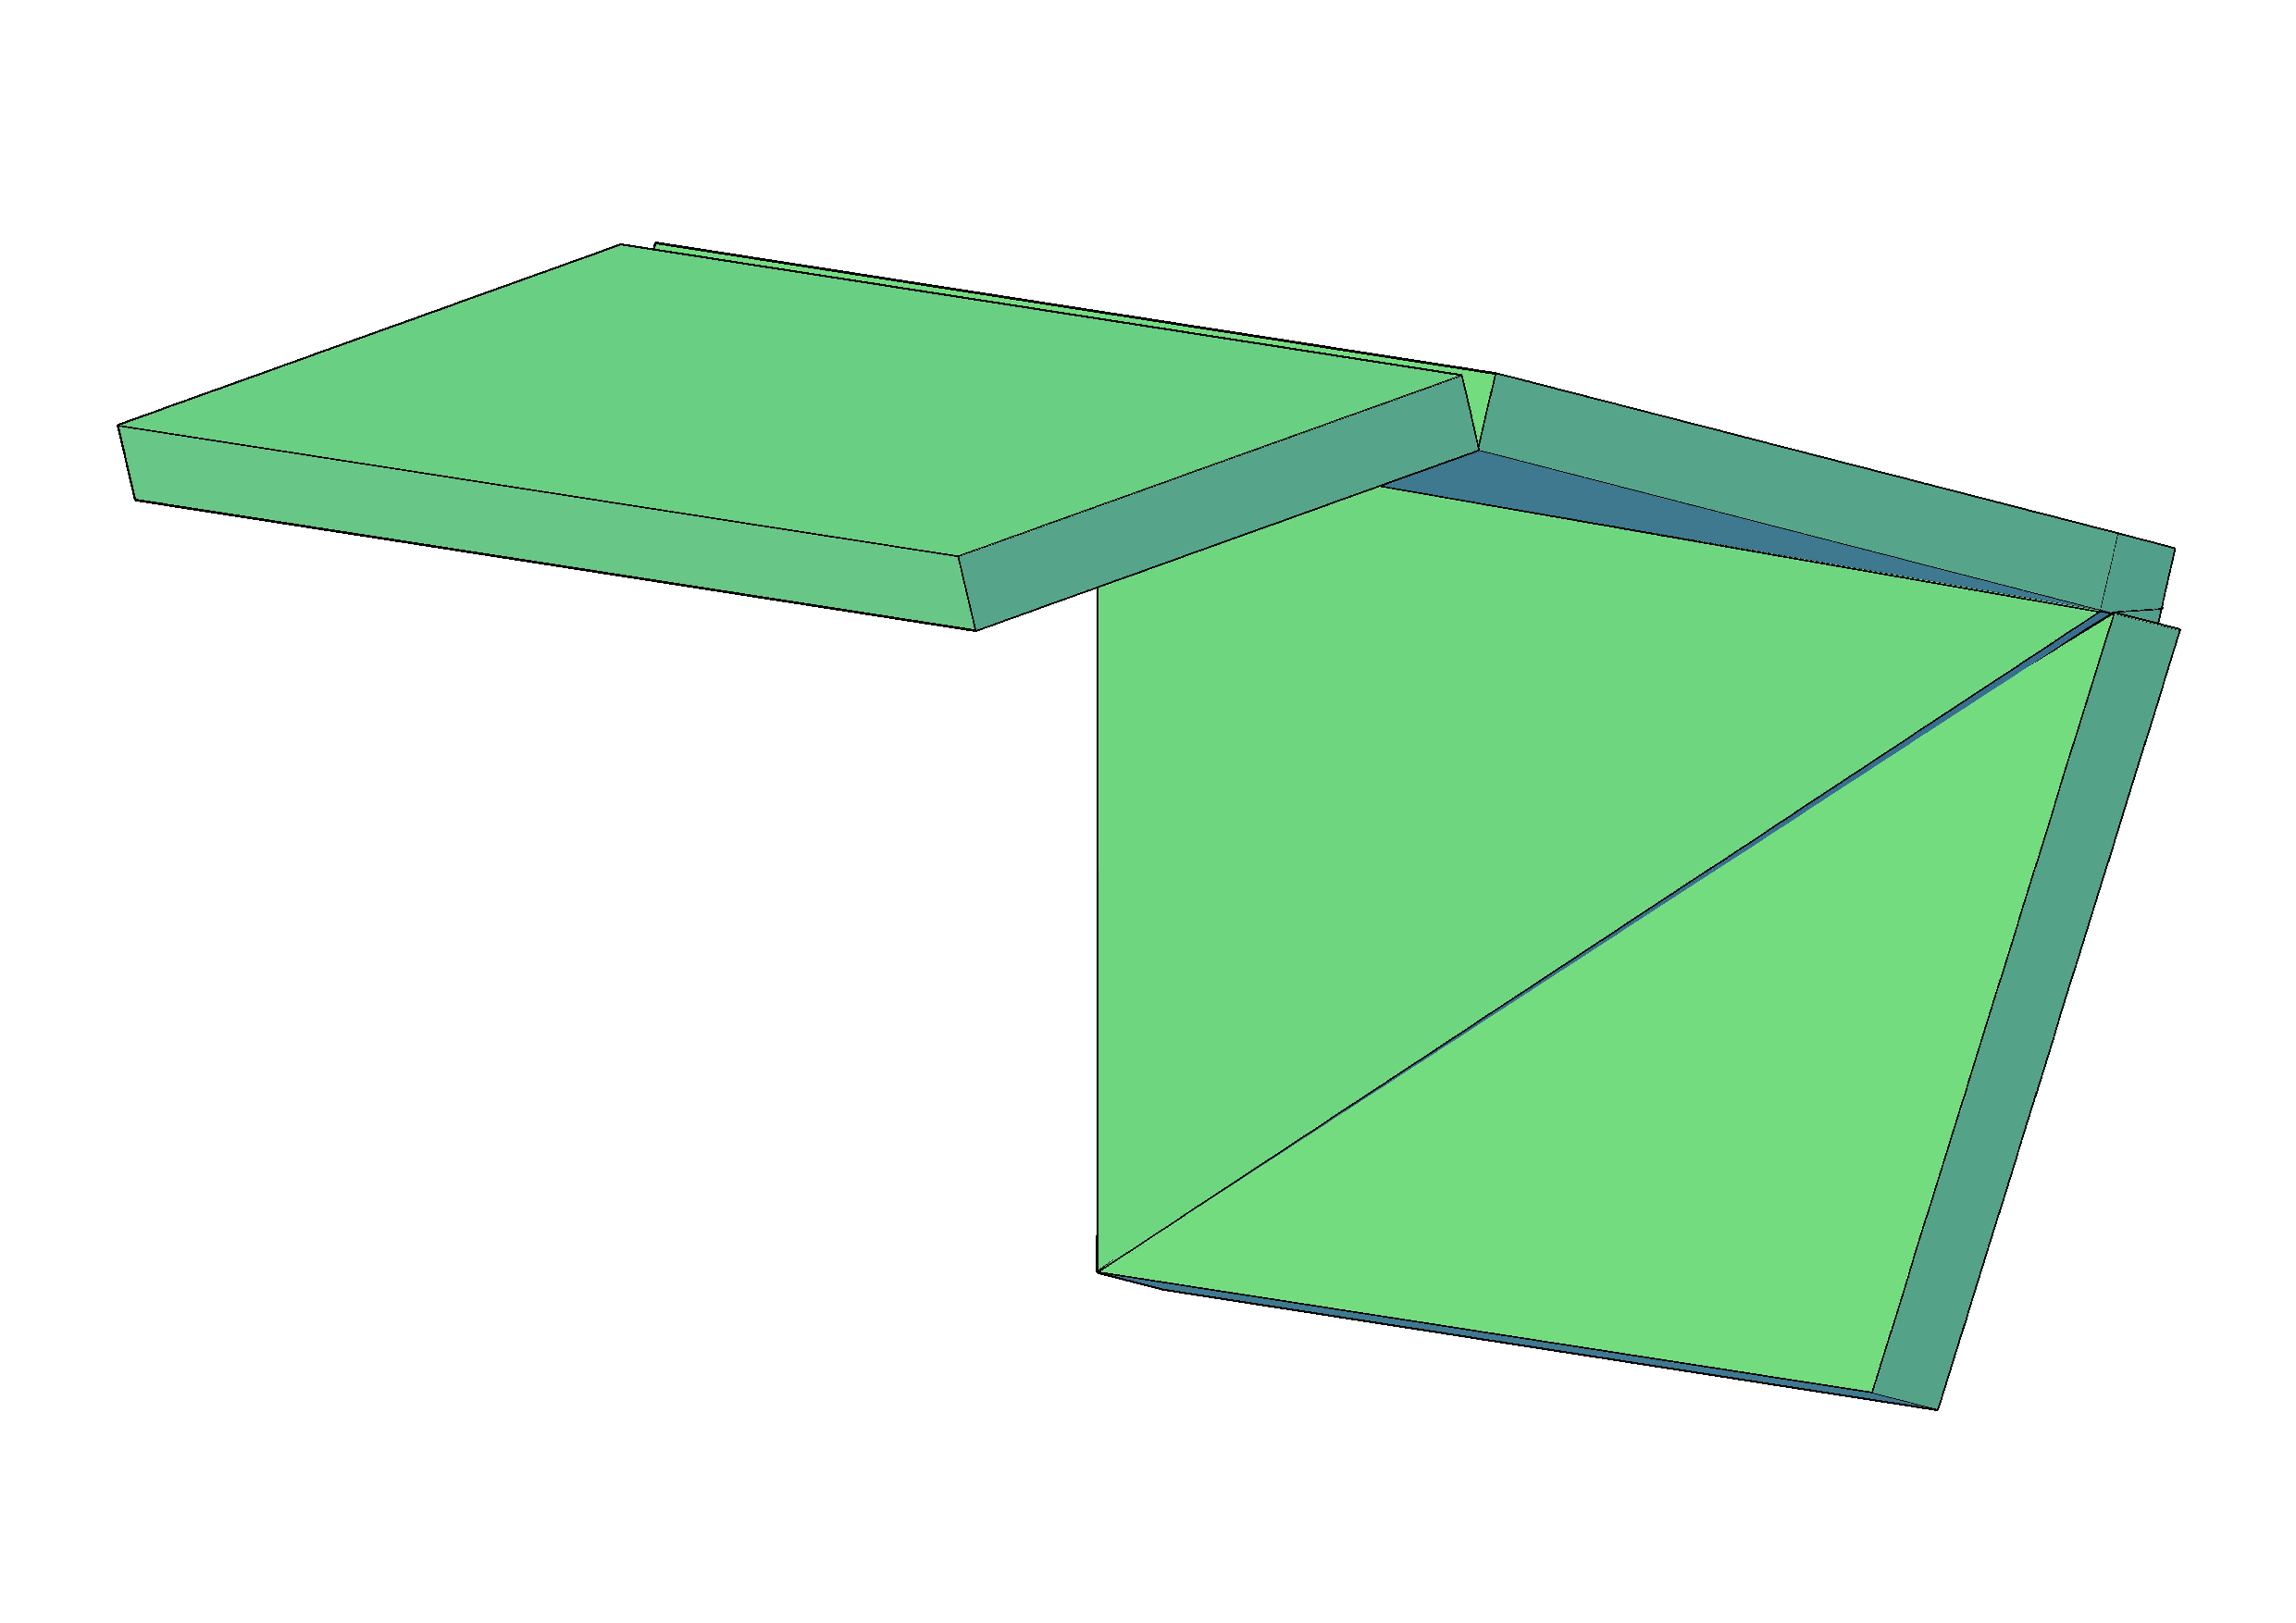
\includegraphics[width=1\linewidth]{1}
	\caption{metti nome immagine qua}
\end{figure}

\begin{figure}[H]
	\centering
	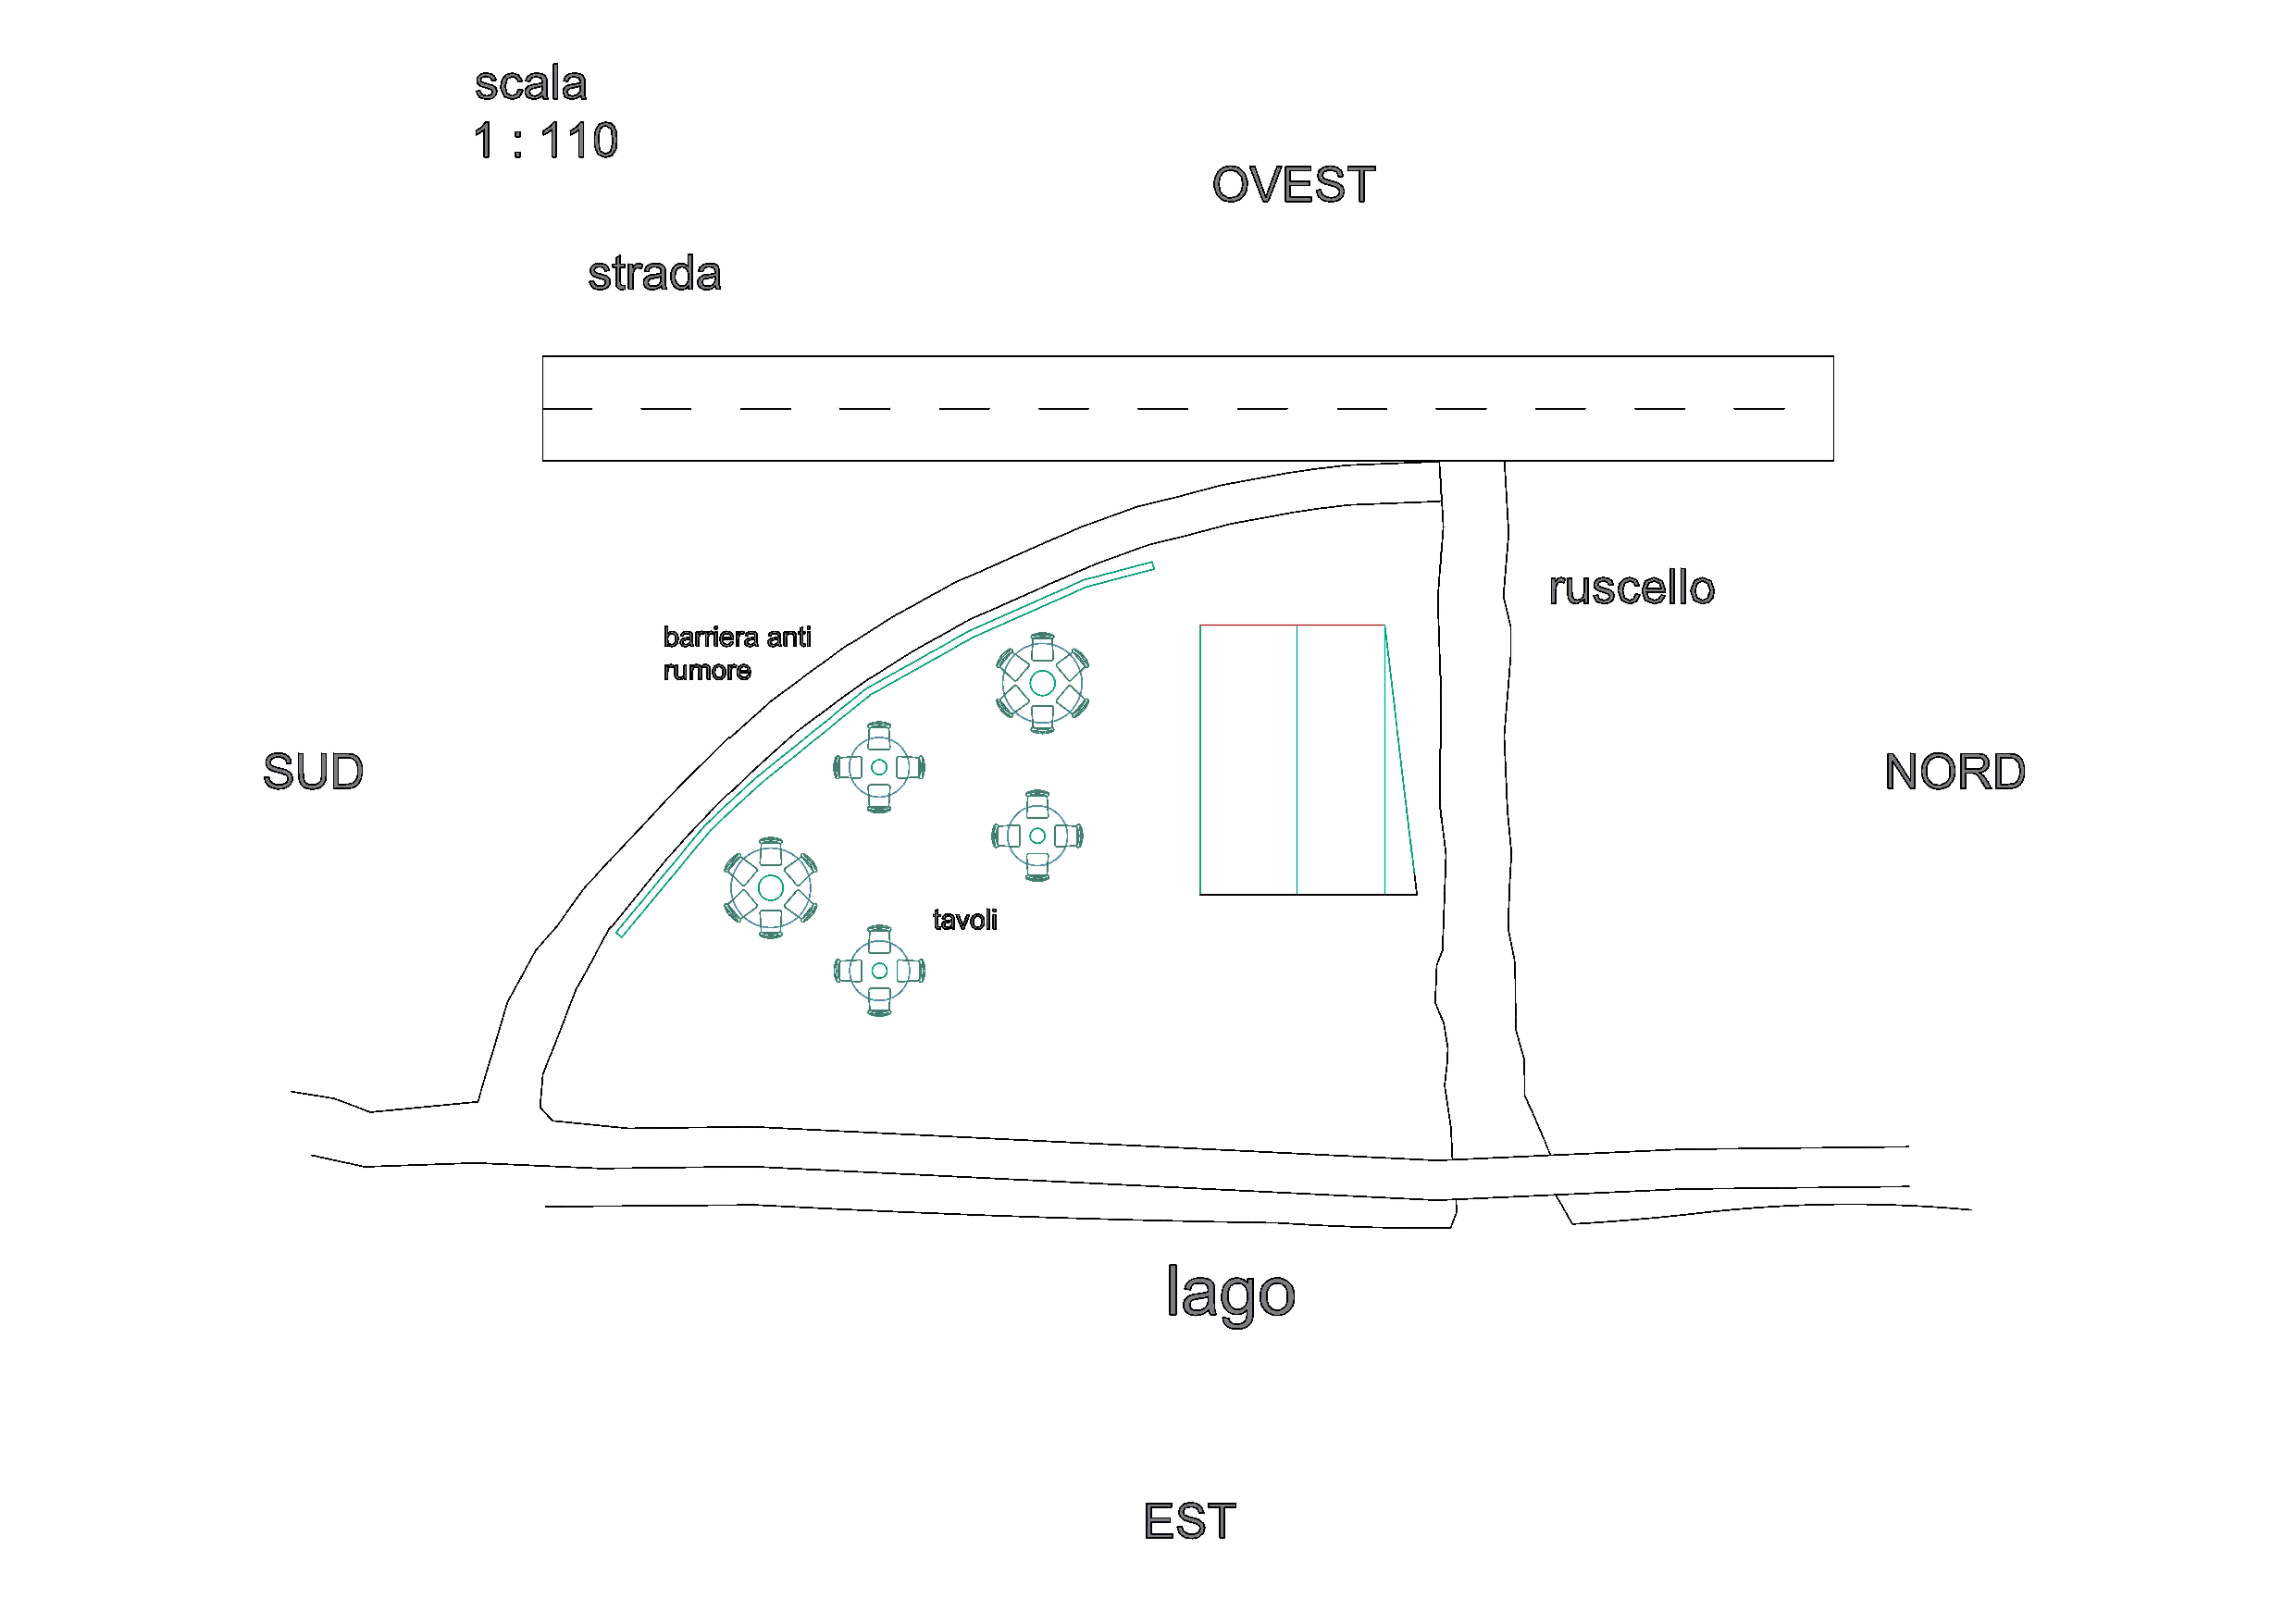
\includegraphics[width=1\linewidth]{2}
	\caption{gasgnasjkl}
\end{figure}

\begin{figure}[H]
	\centering
	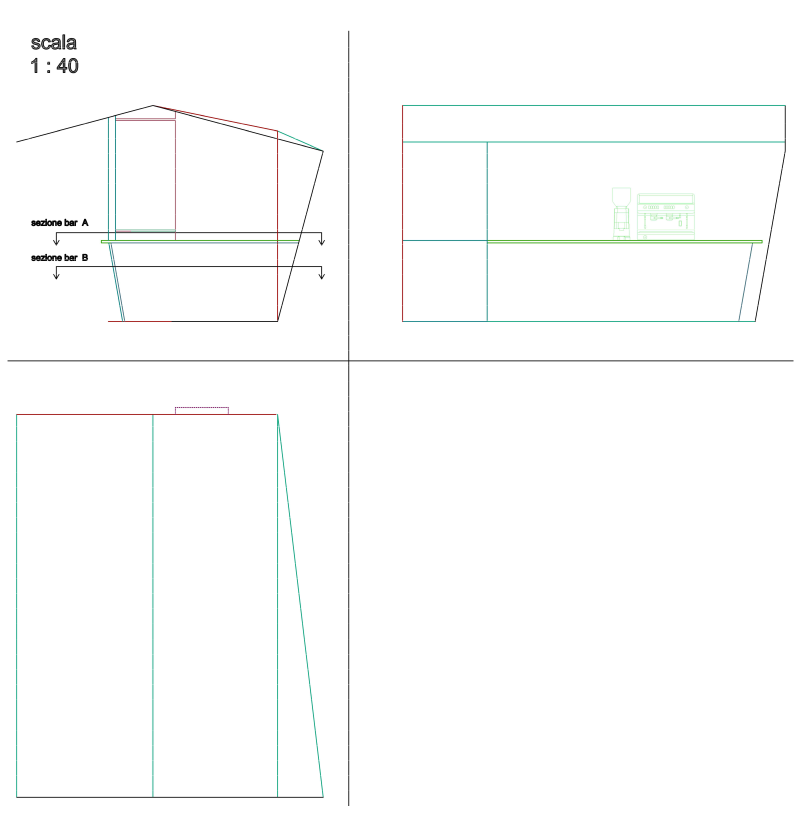
\includegraphics[width=1\linewidth]{3}
\end{figure}

\begin{figure}[H]
	\centering
	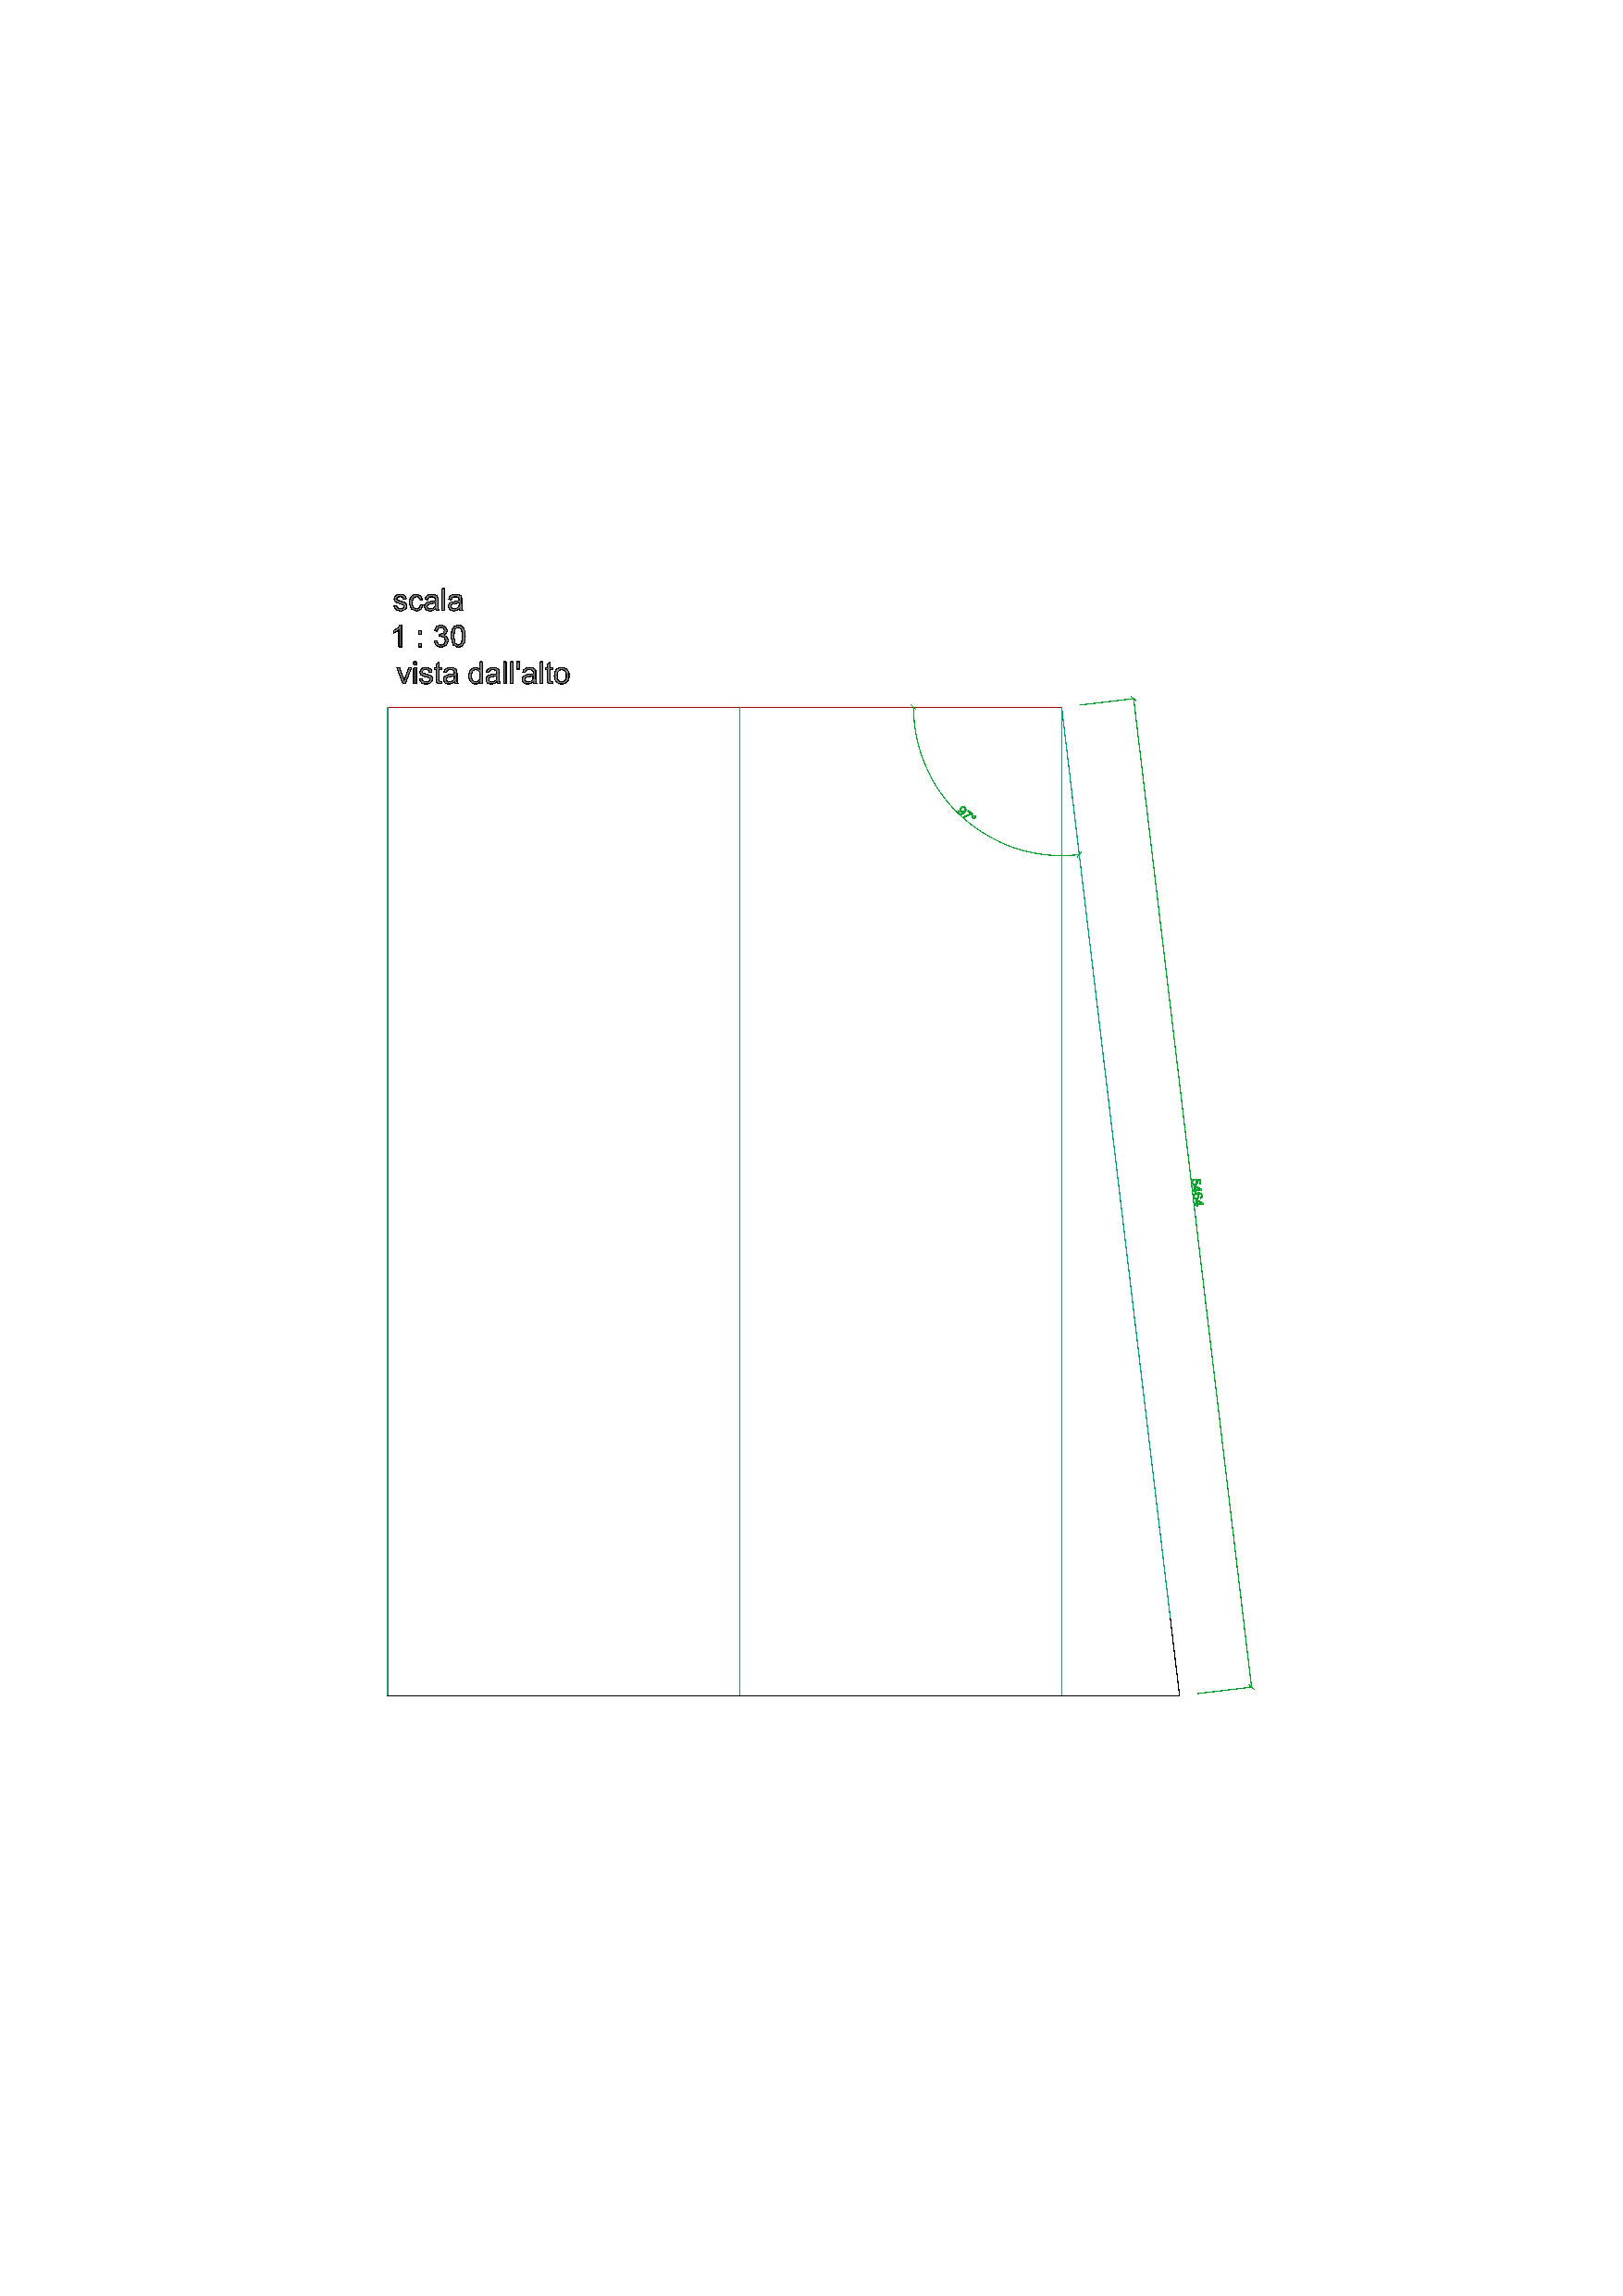
\includegraphics[width=1\linewidth]{4}
\end{figure}

\newpage
\begin{figure}[H]
	\centering
	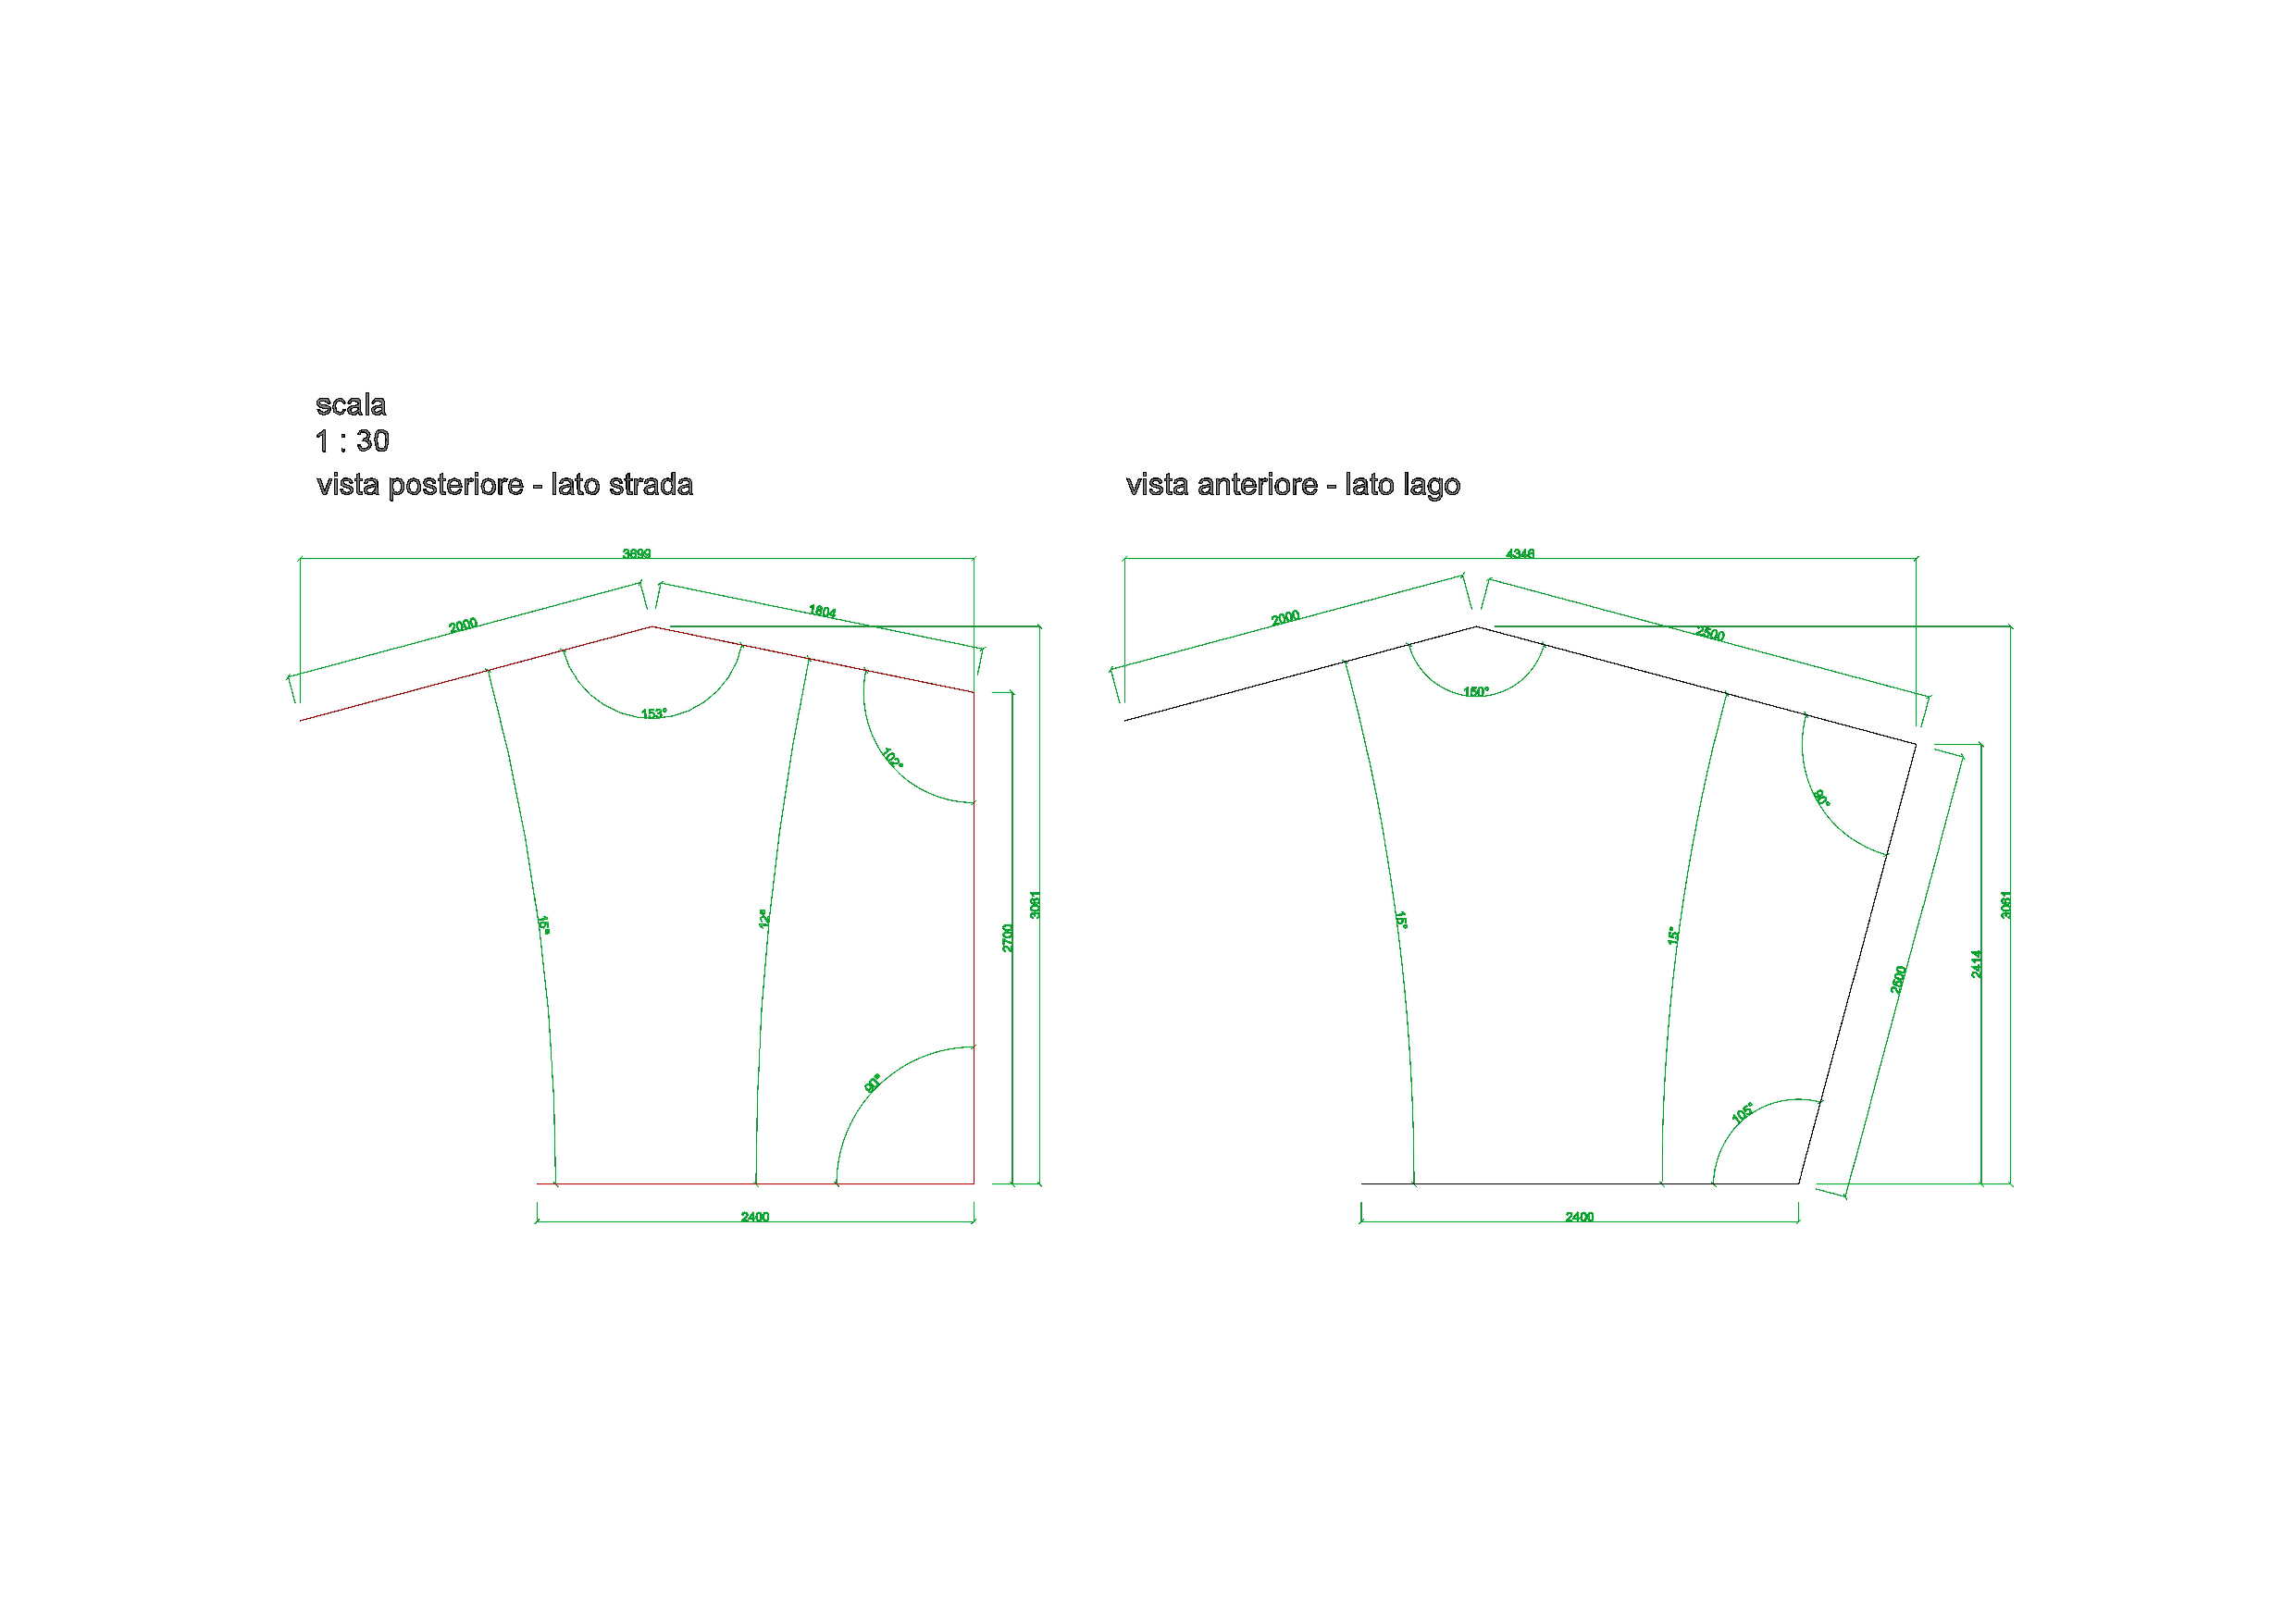
\includegraphics[width=0.8\linewidth]{5}
\end{figure}

\begin{figure}[H]
	\centering
	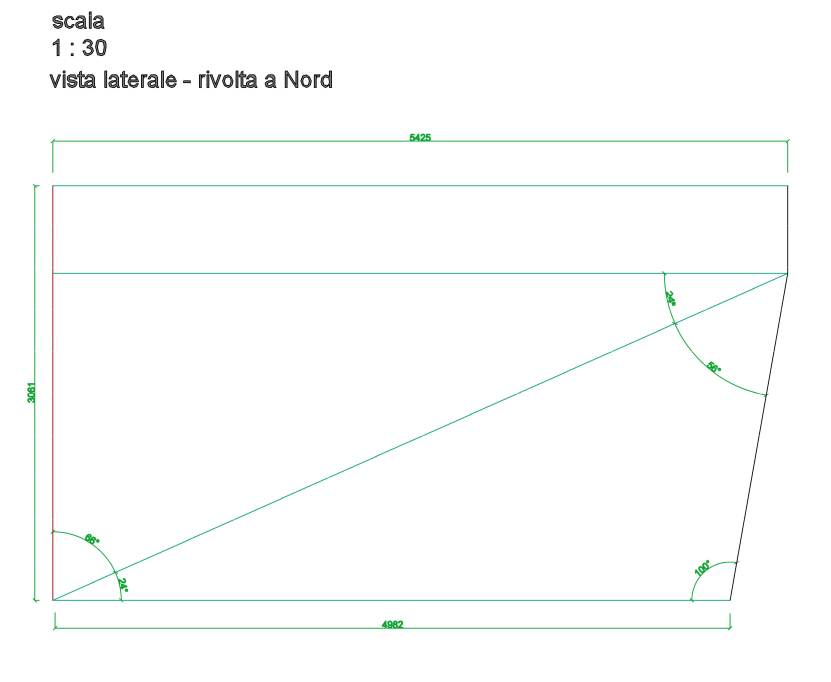
\includegraphics[width=0.7\linewidth]{6}
\end{figure}

\begin{figure}[H]
	\centering
	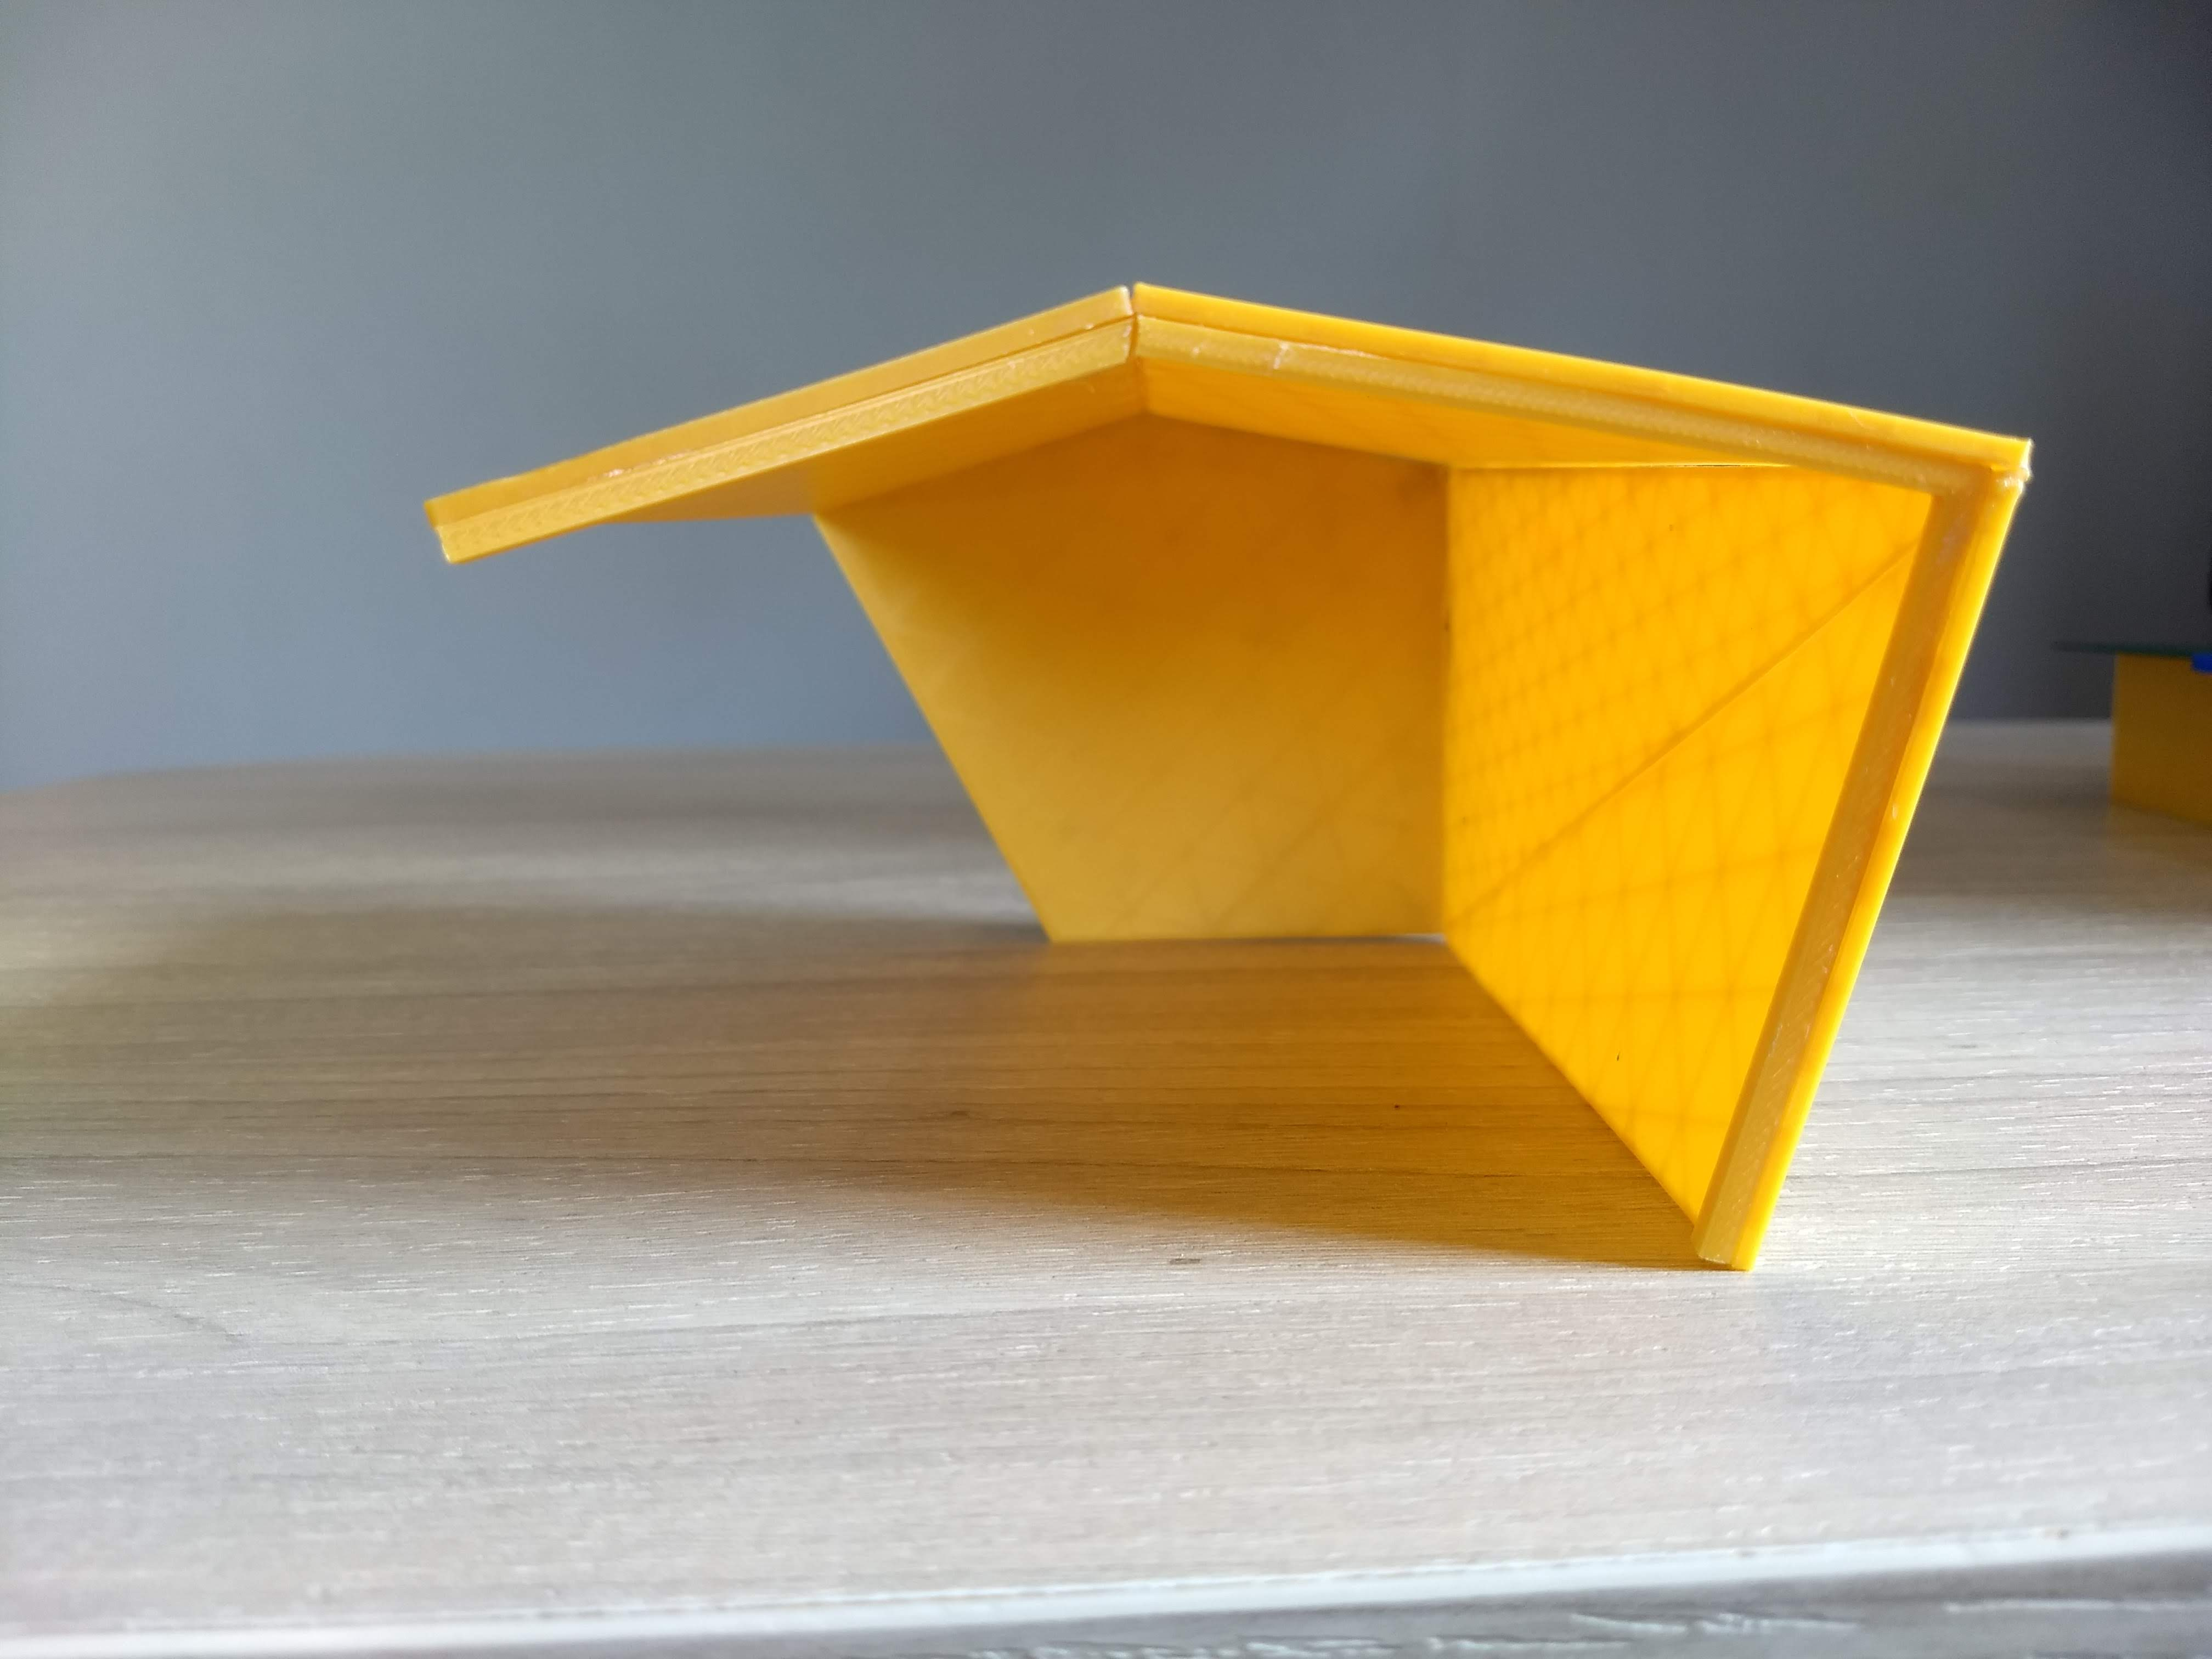
\includegraphics[width=1\linewidth]{7}
\end{figure}

\begin{figure}[H]
	\centering
	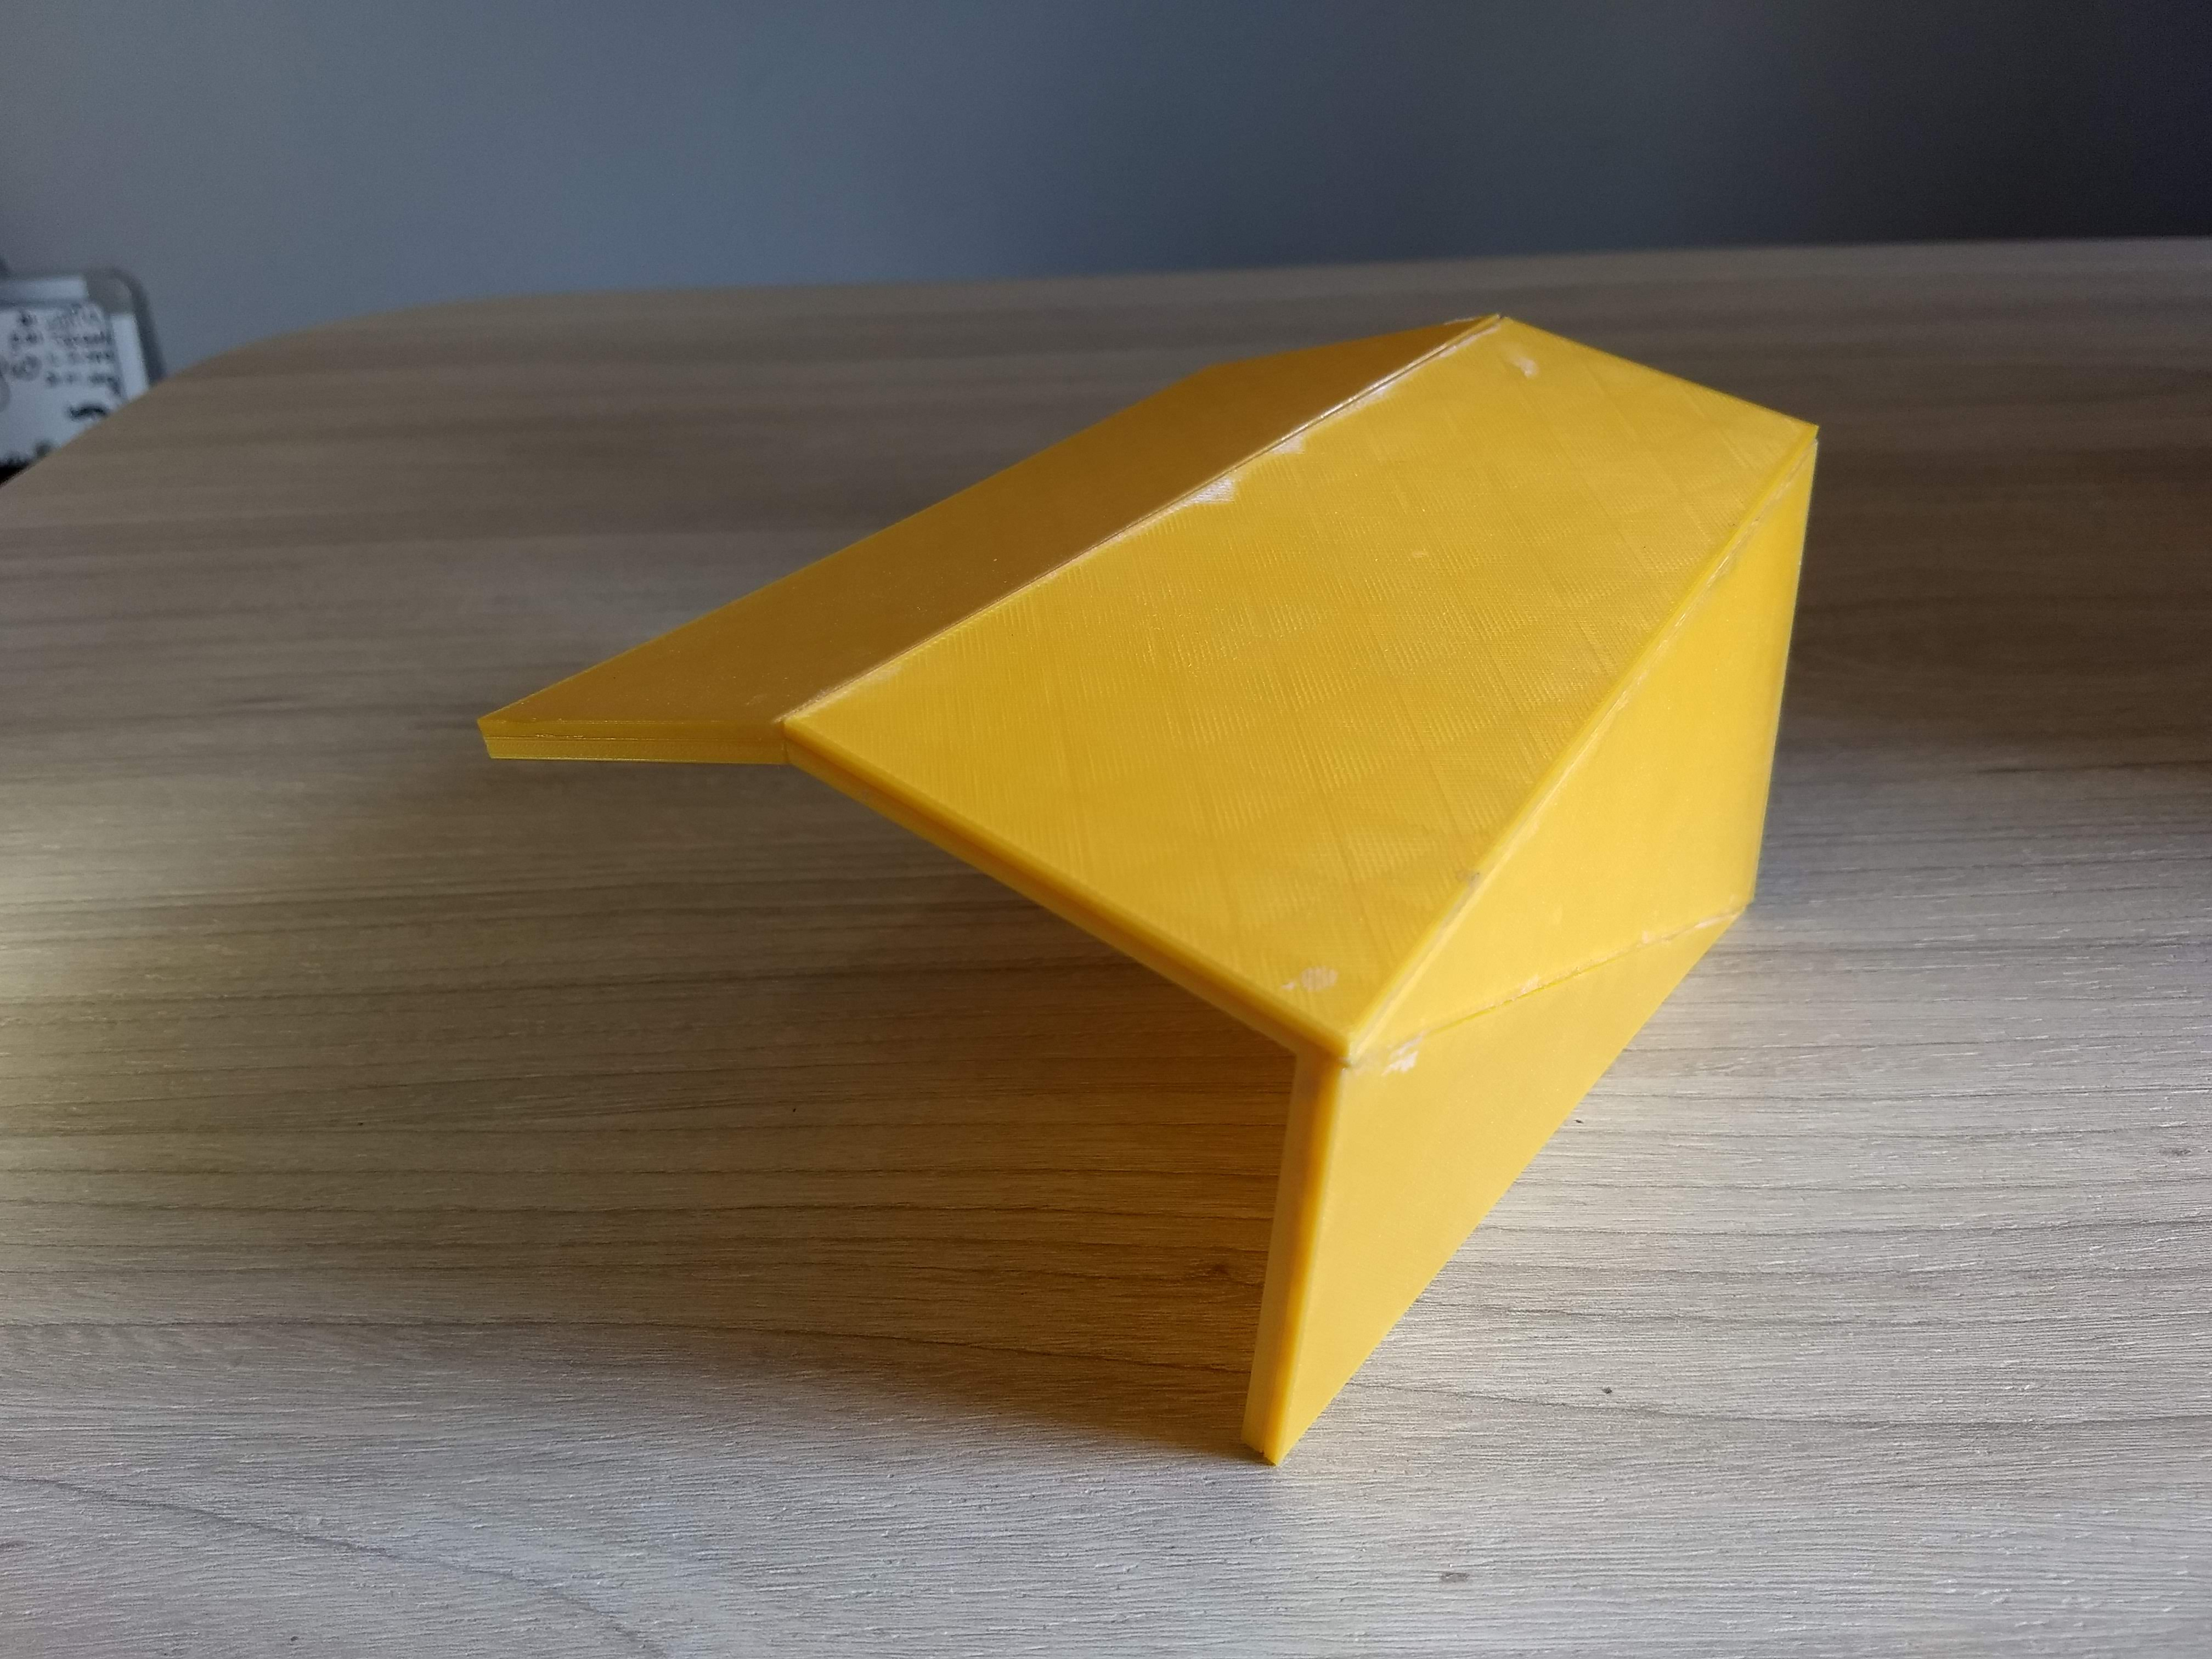
\includegraphics[width=1\linewidth]{8}
\end{figure}

\begin{figure}[H]
	\centering
	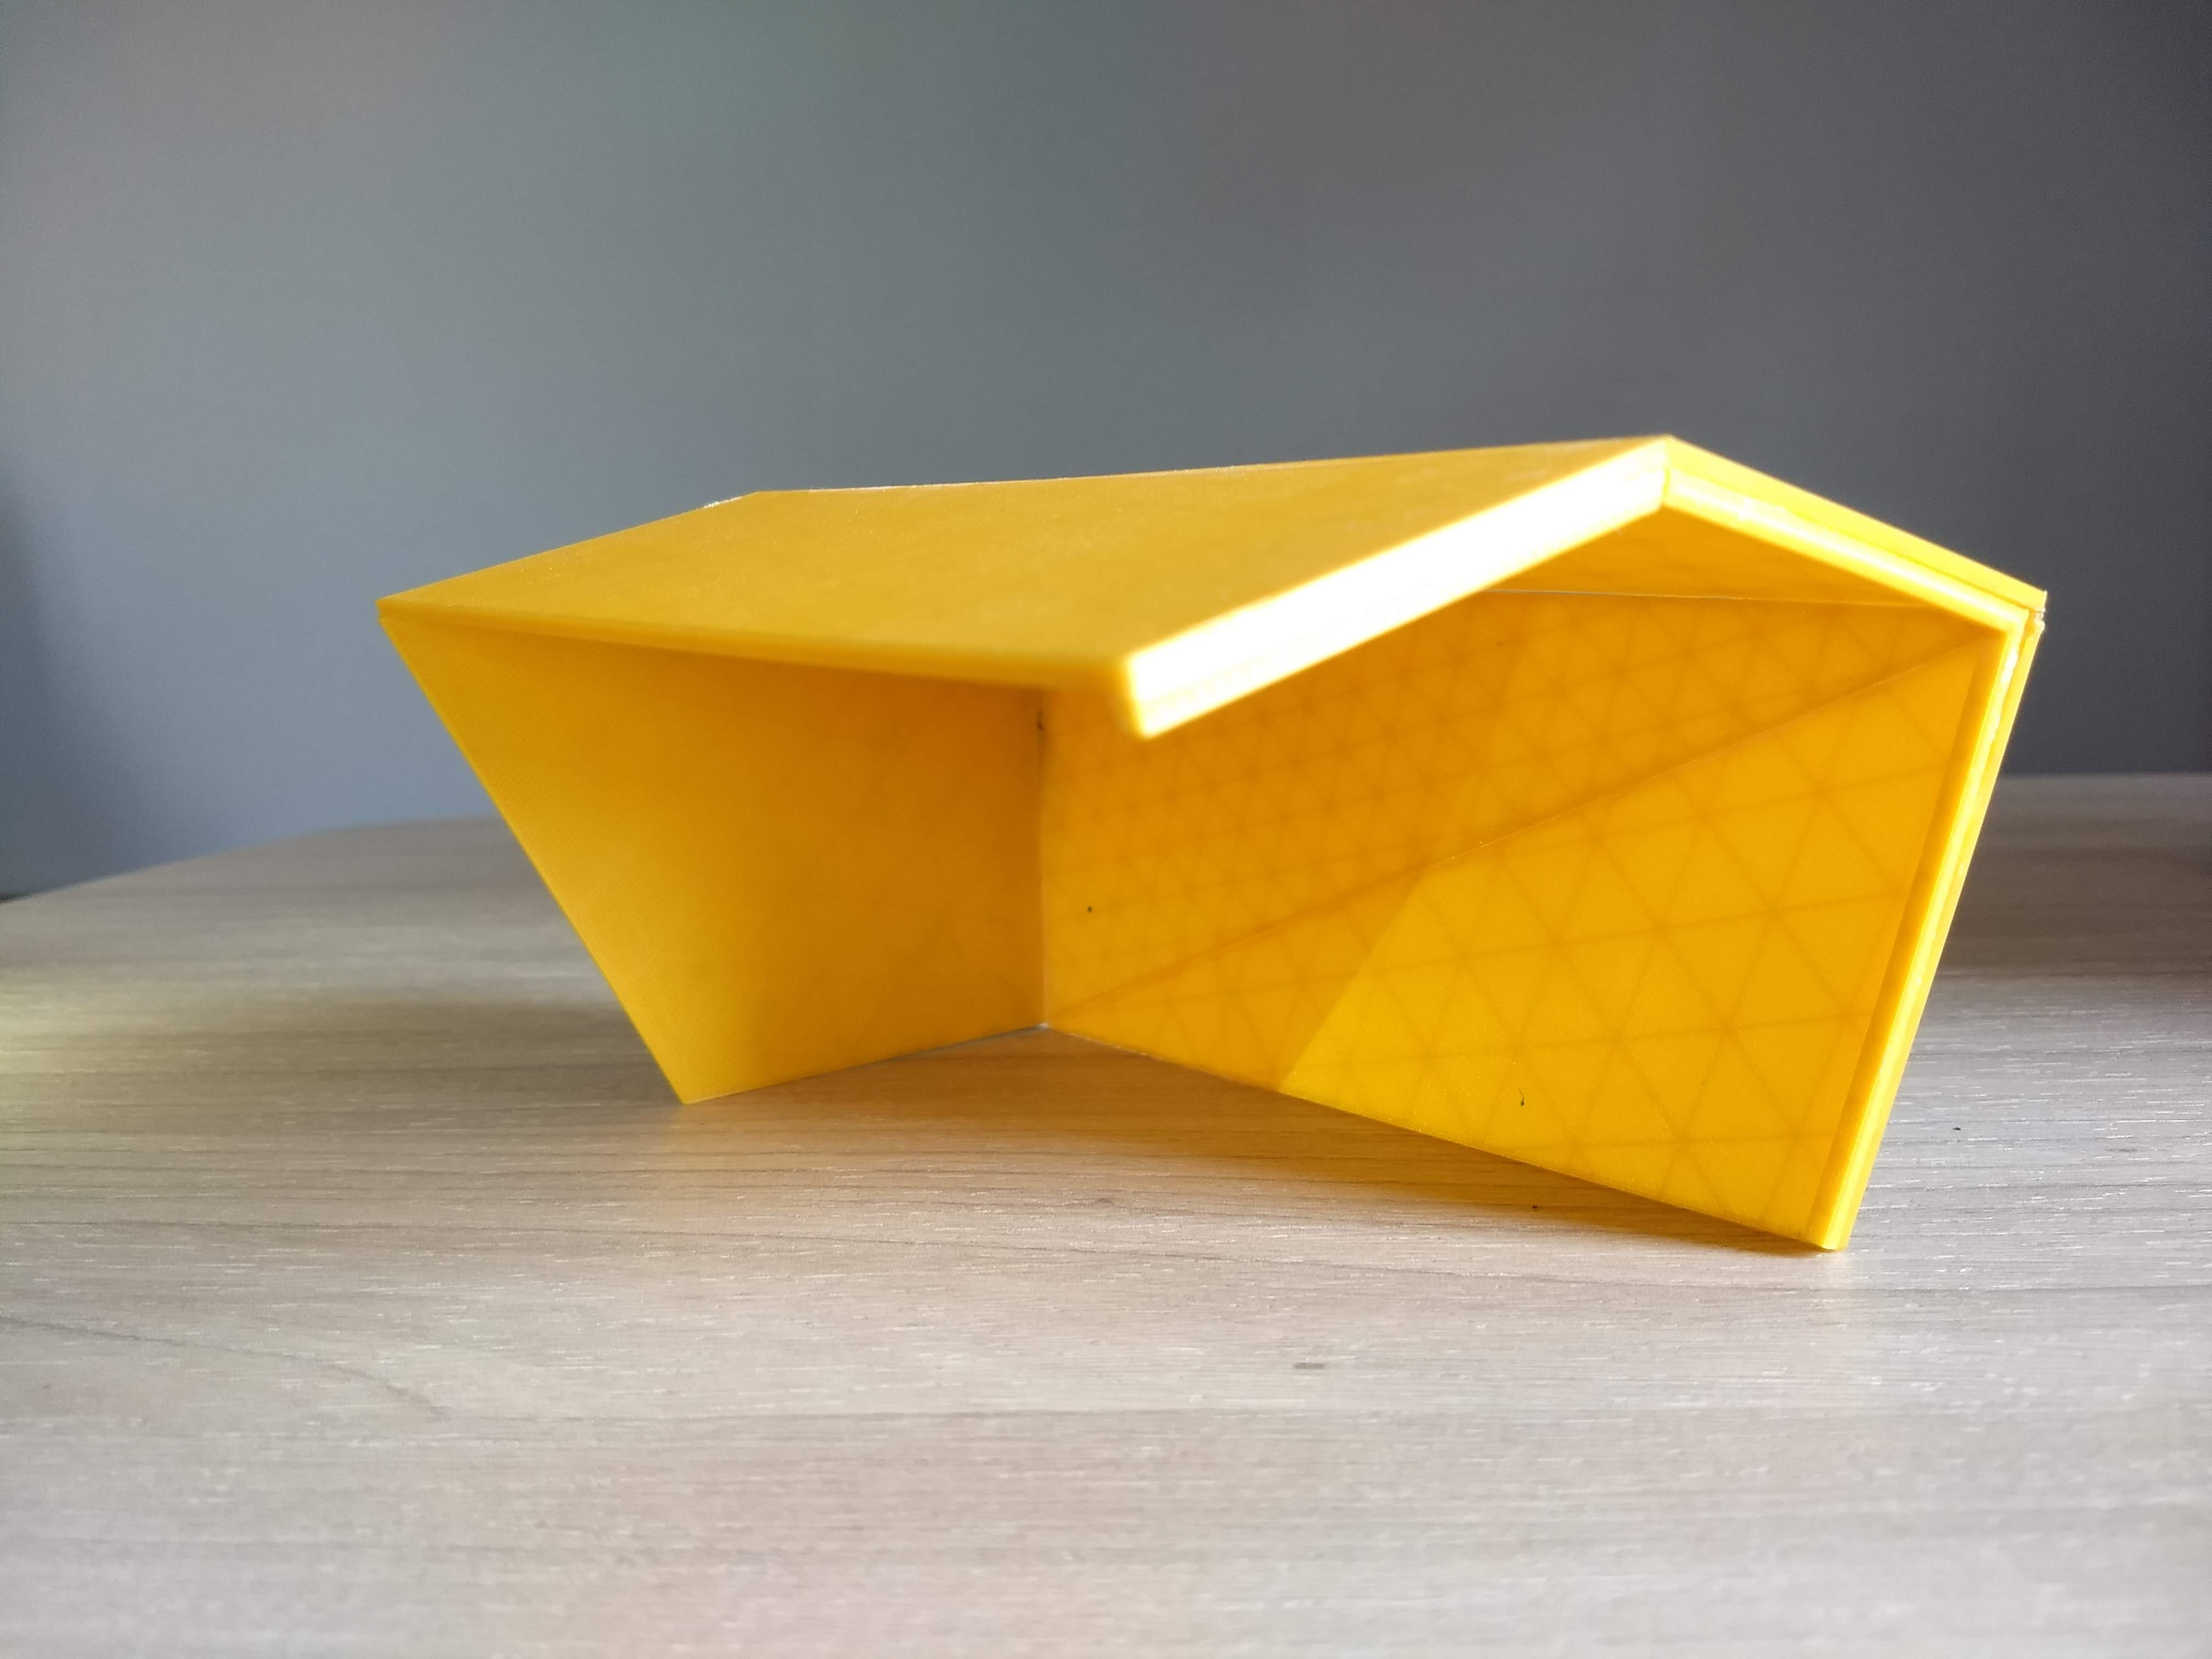
\includegraphics[width=1\linewidth]{9}
\end{figure}

\begin{figure}[H]
	\centering
	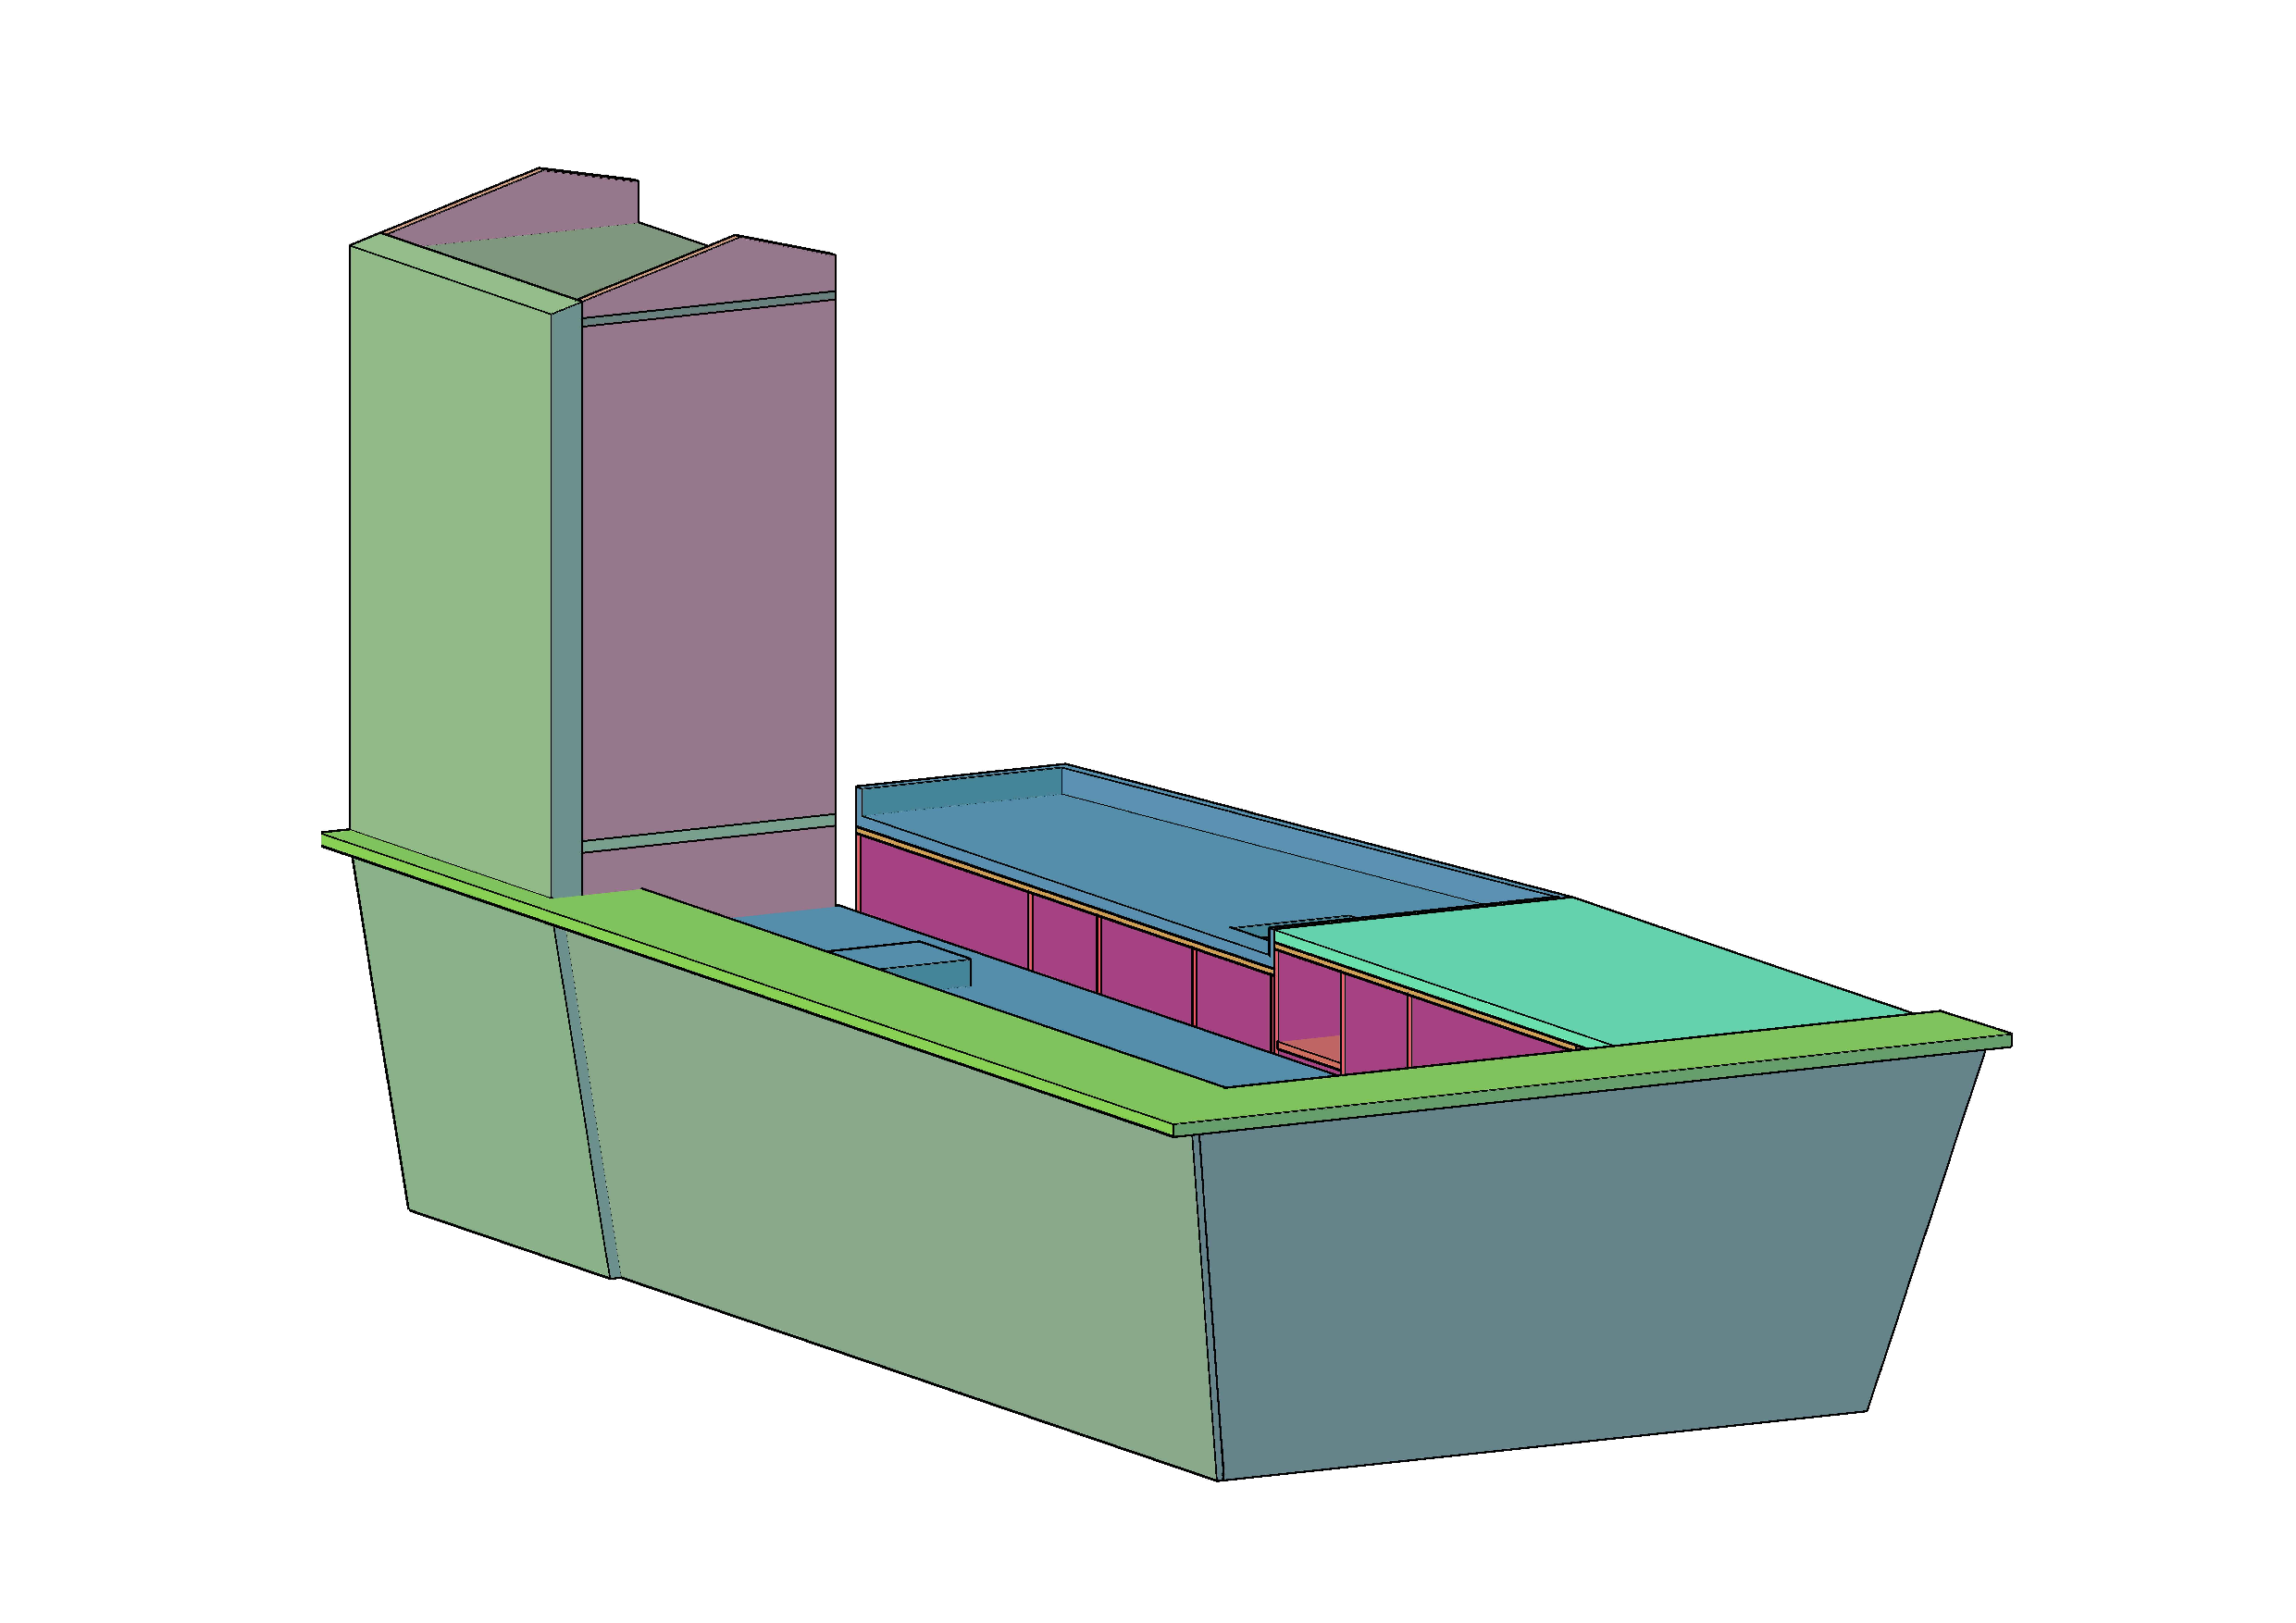
\includegraphics[width=1\linewidth]{10}
\end{figure}

% ----------------------


\begin{figure}[H]
	\centering
	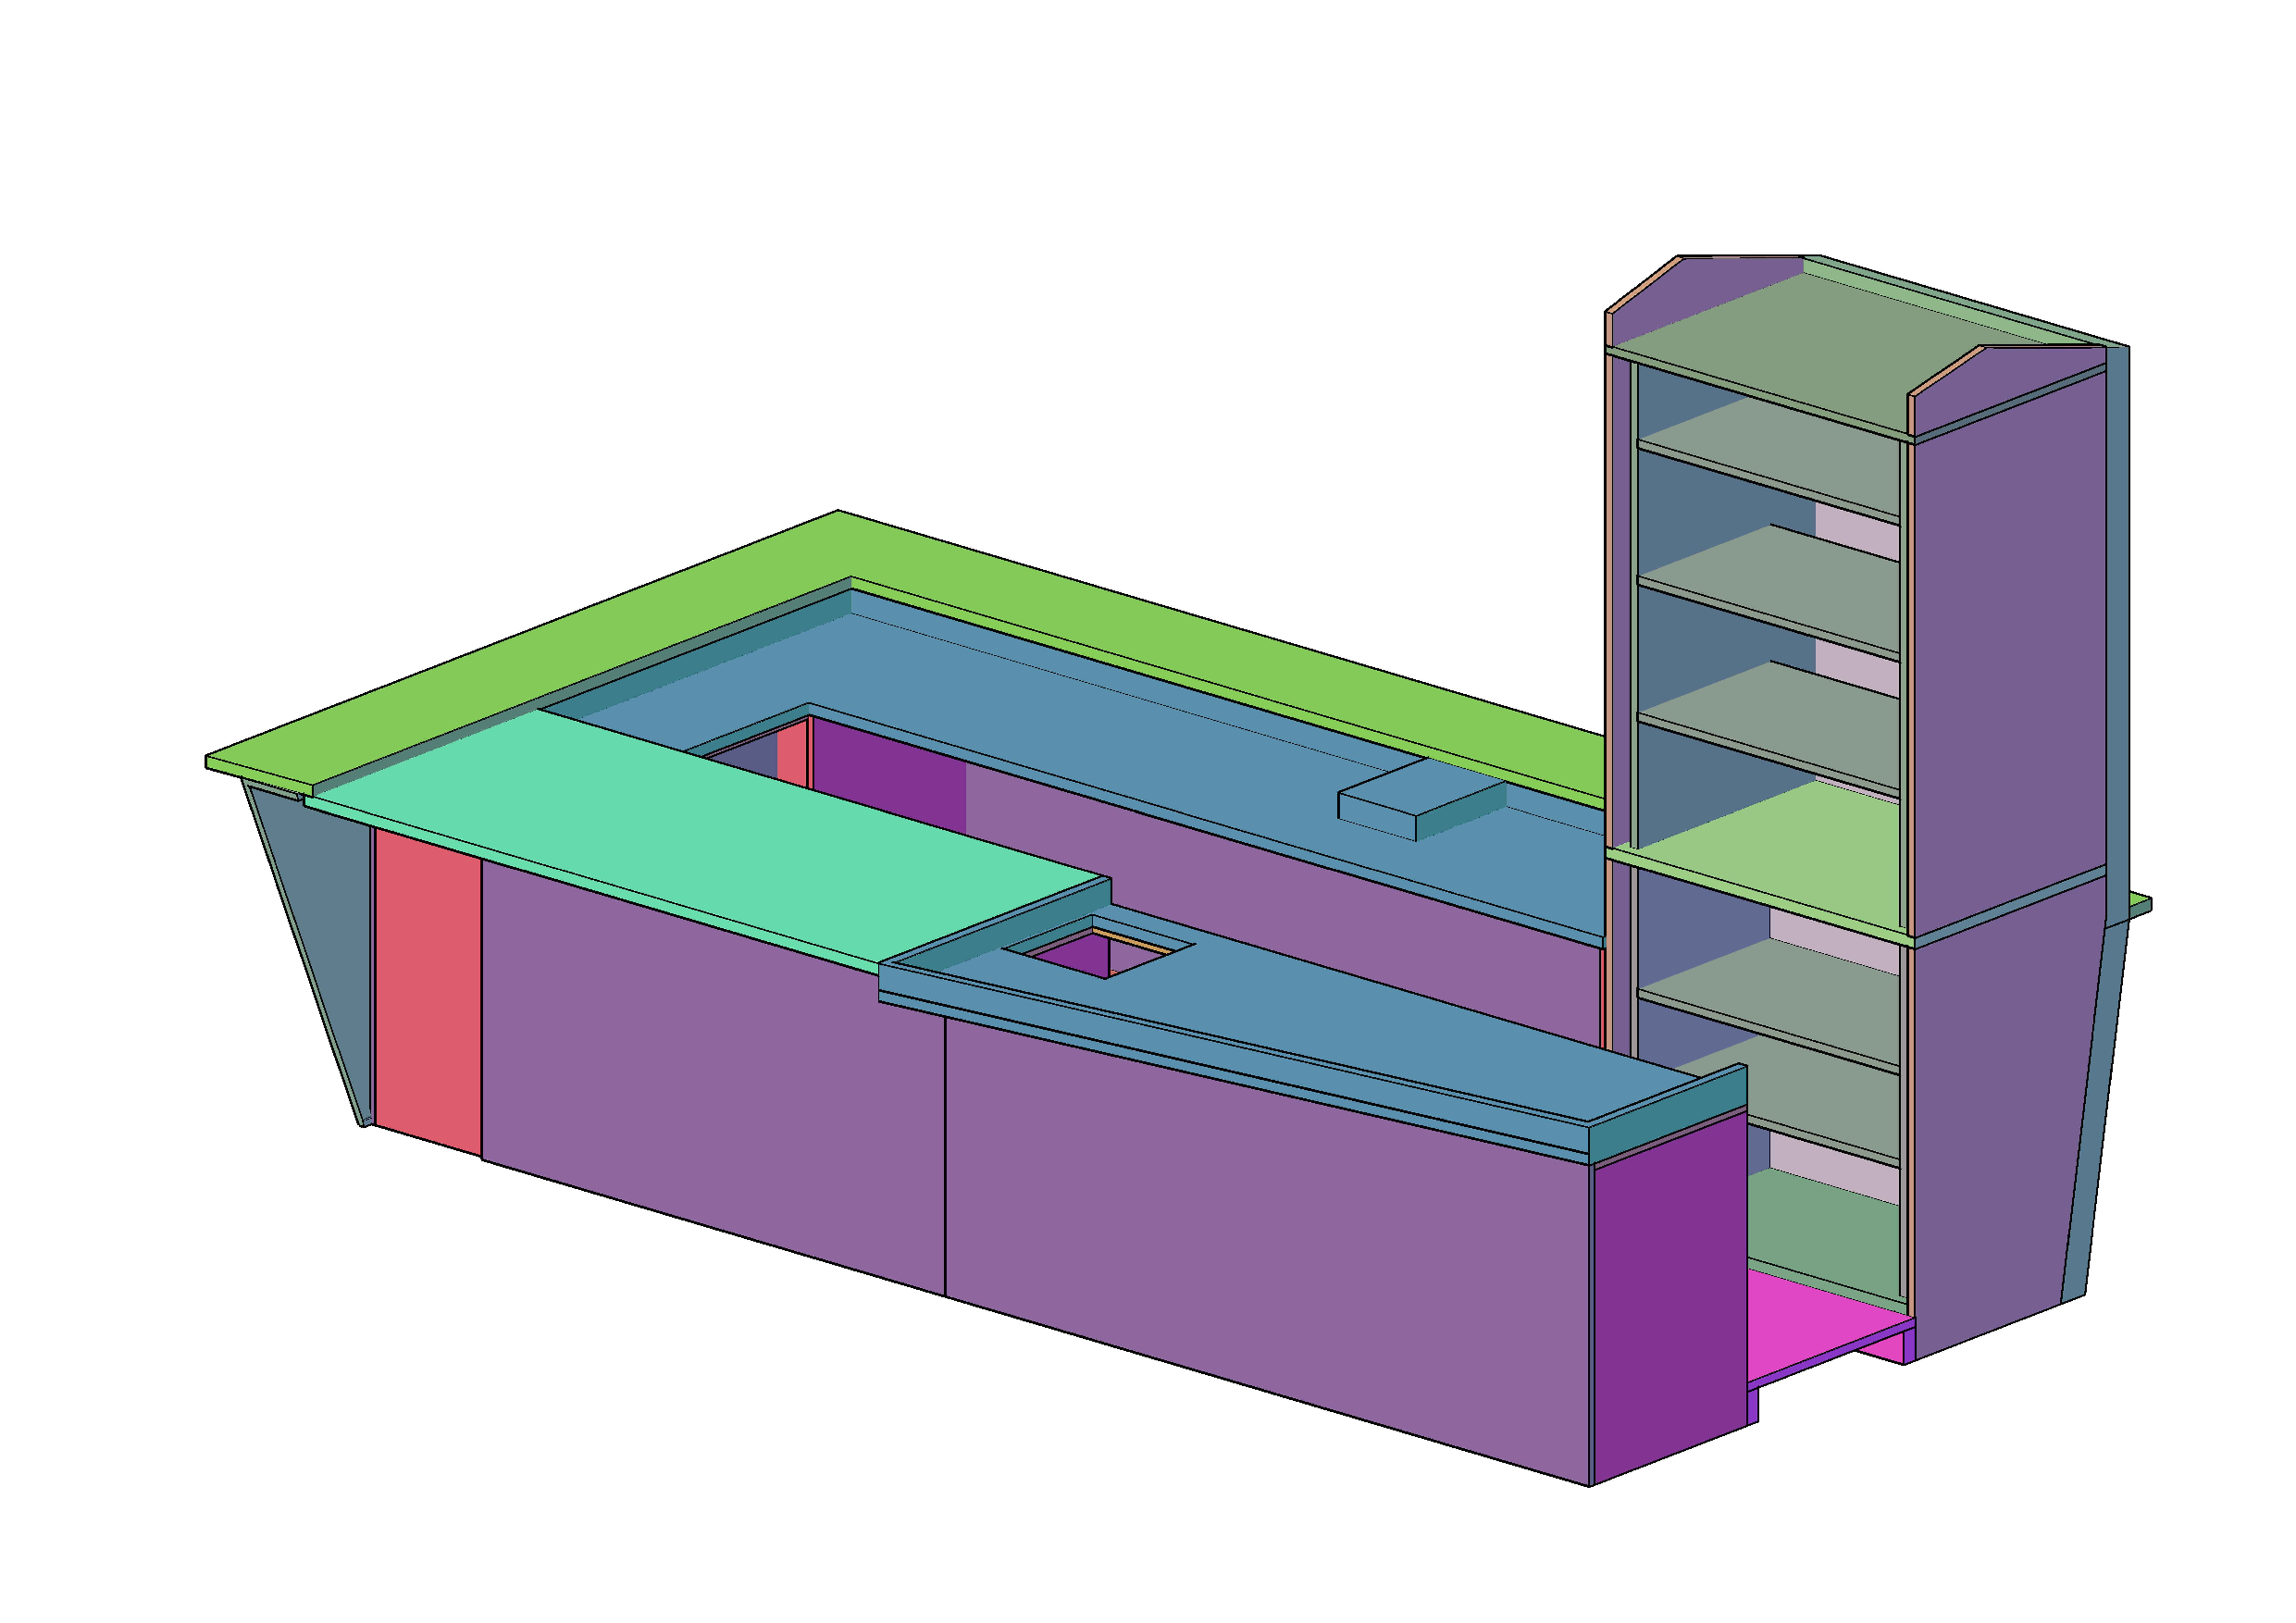
\includegraphics[width=1\linewidth]{11}
\end{figure}


\begin{figure}[H]
	\centering
	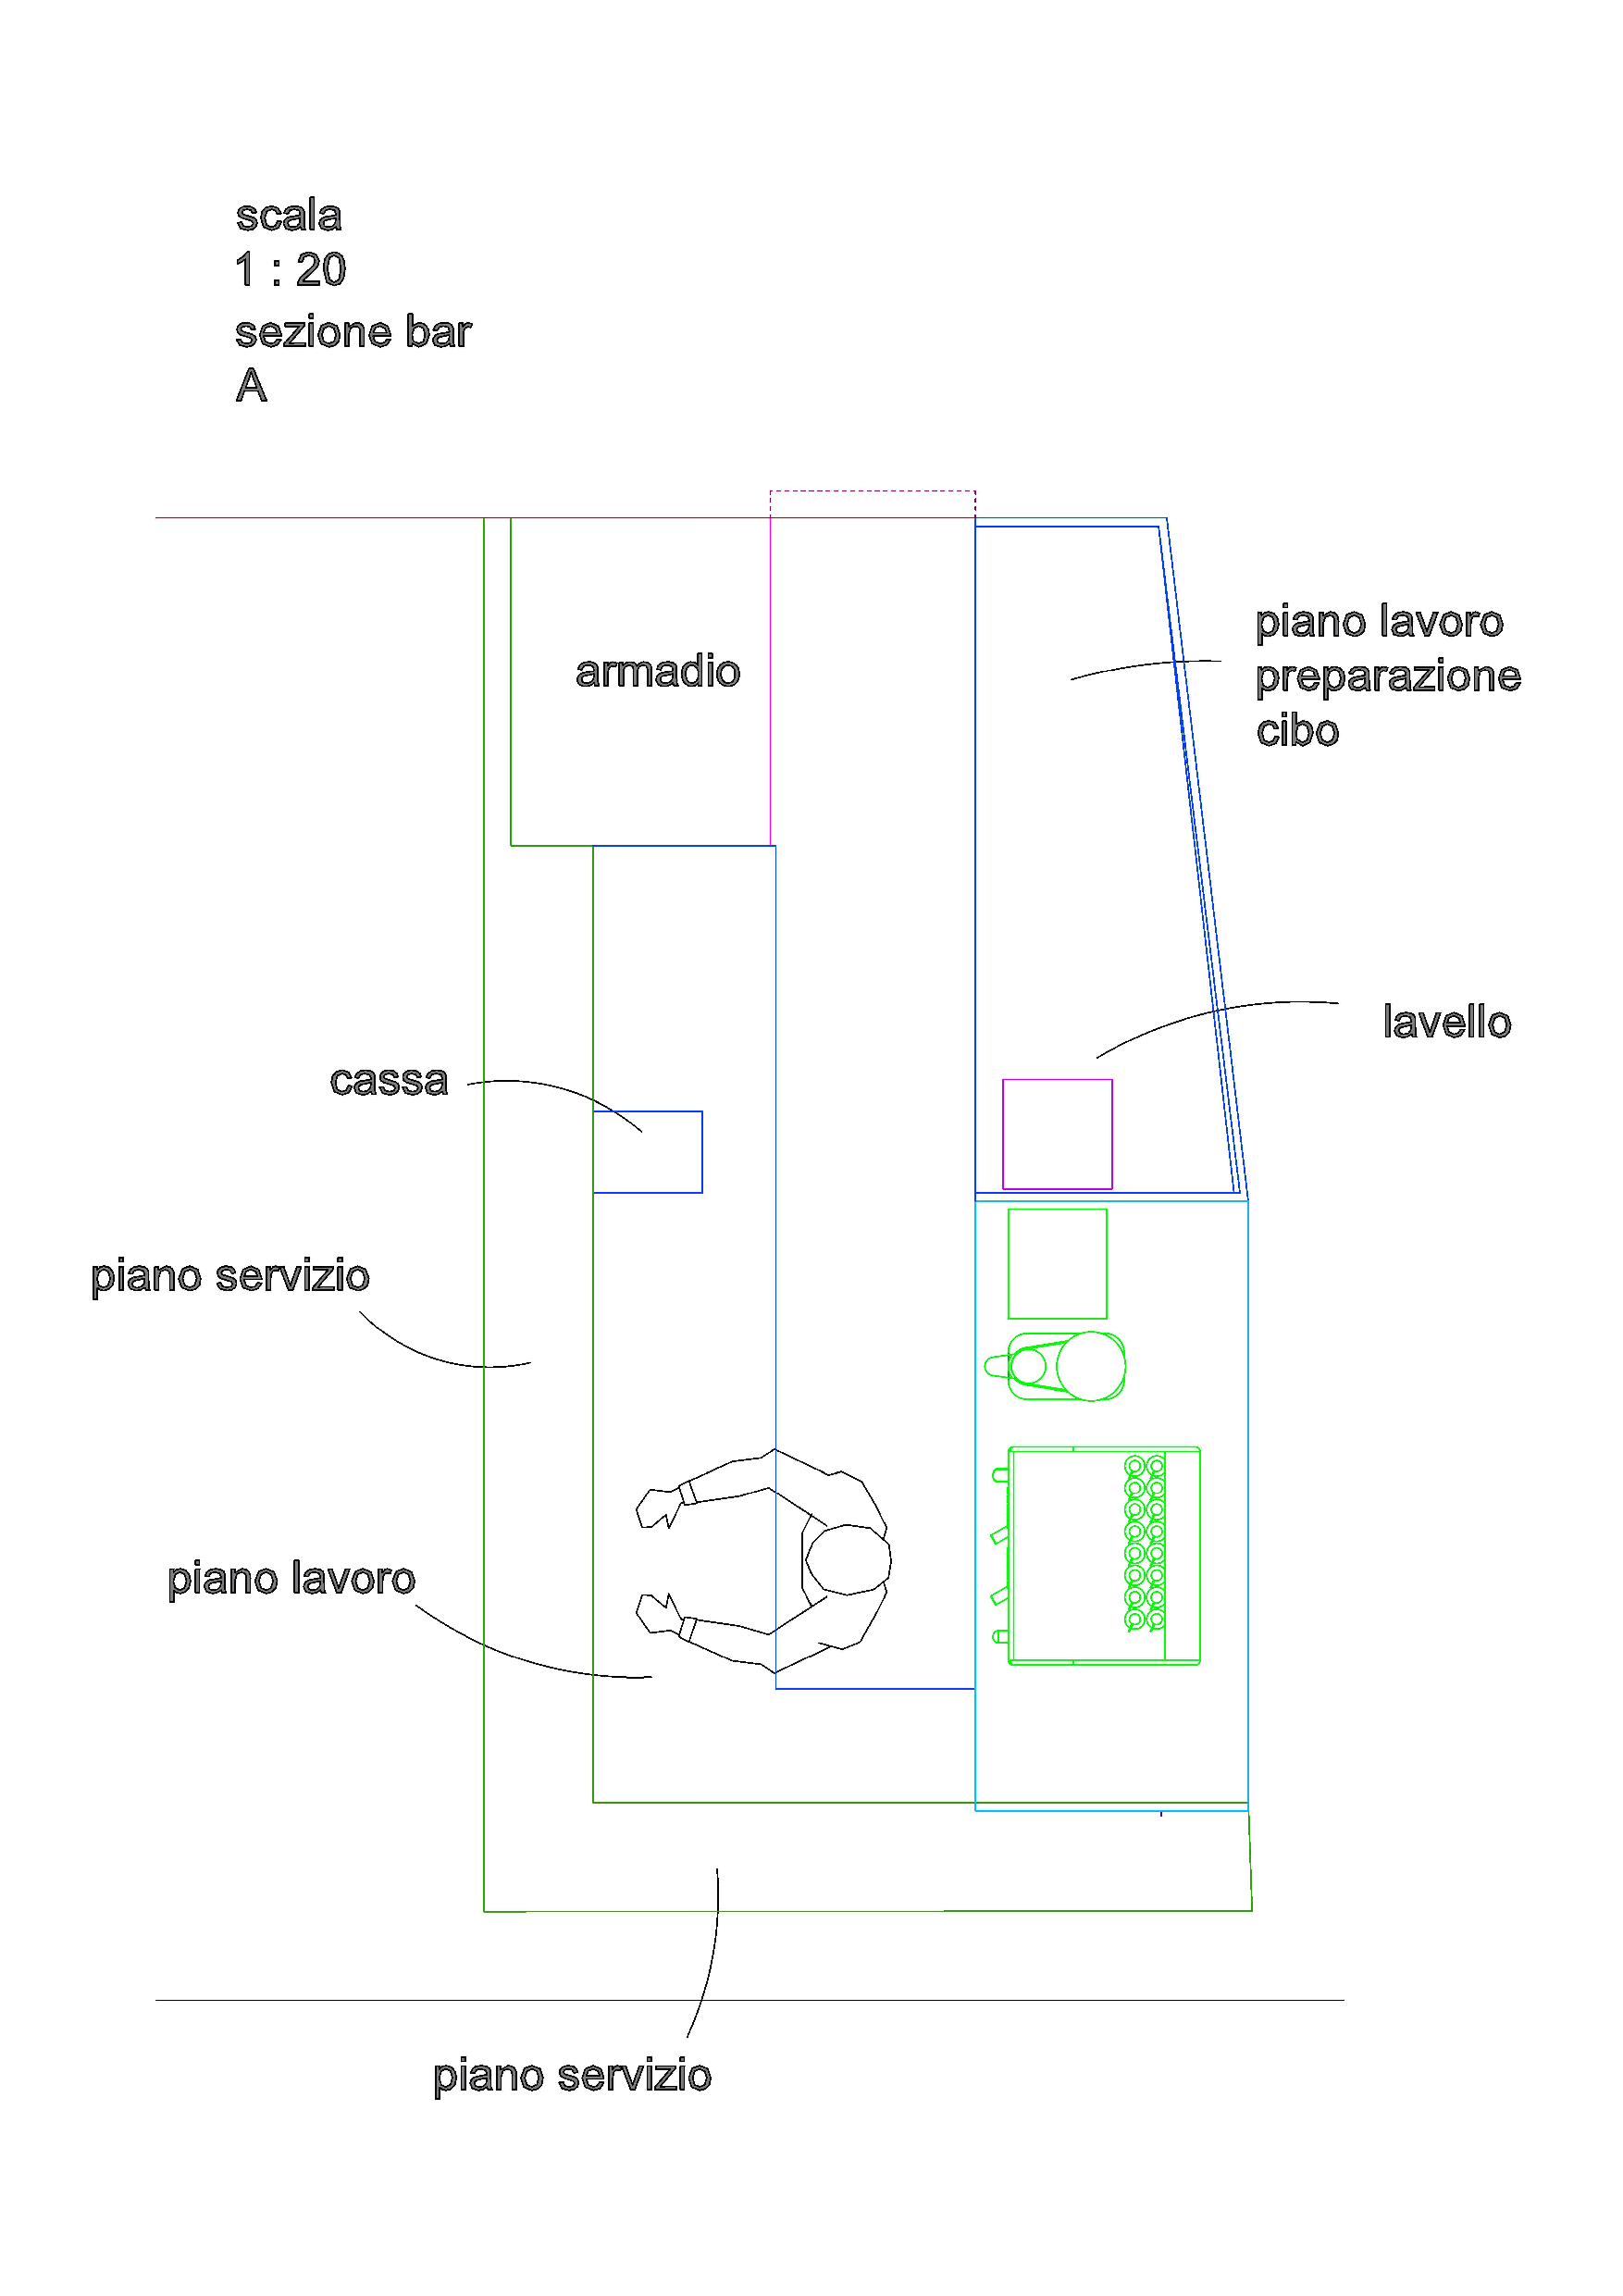
\includegraphics[width=1\linewidth]{12}
\end{figure}

\begin{figure}[H]
	\centering
	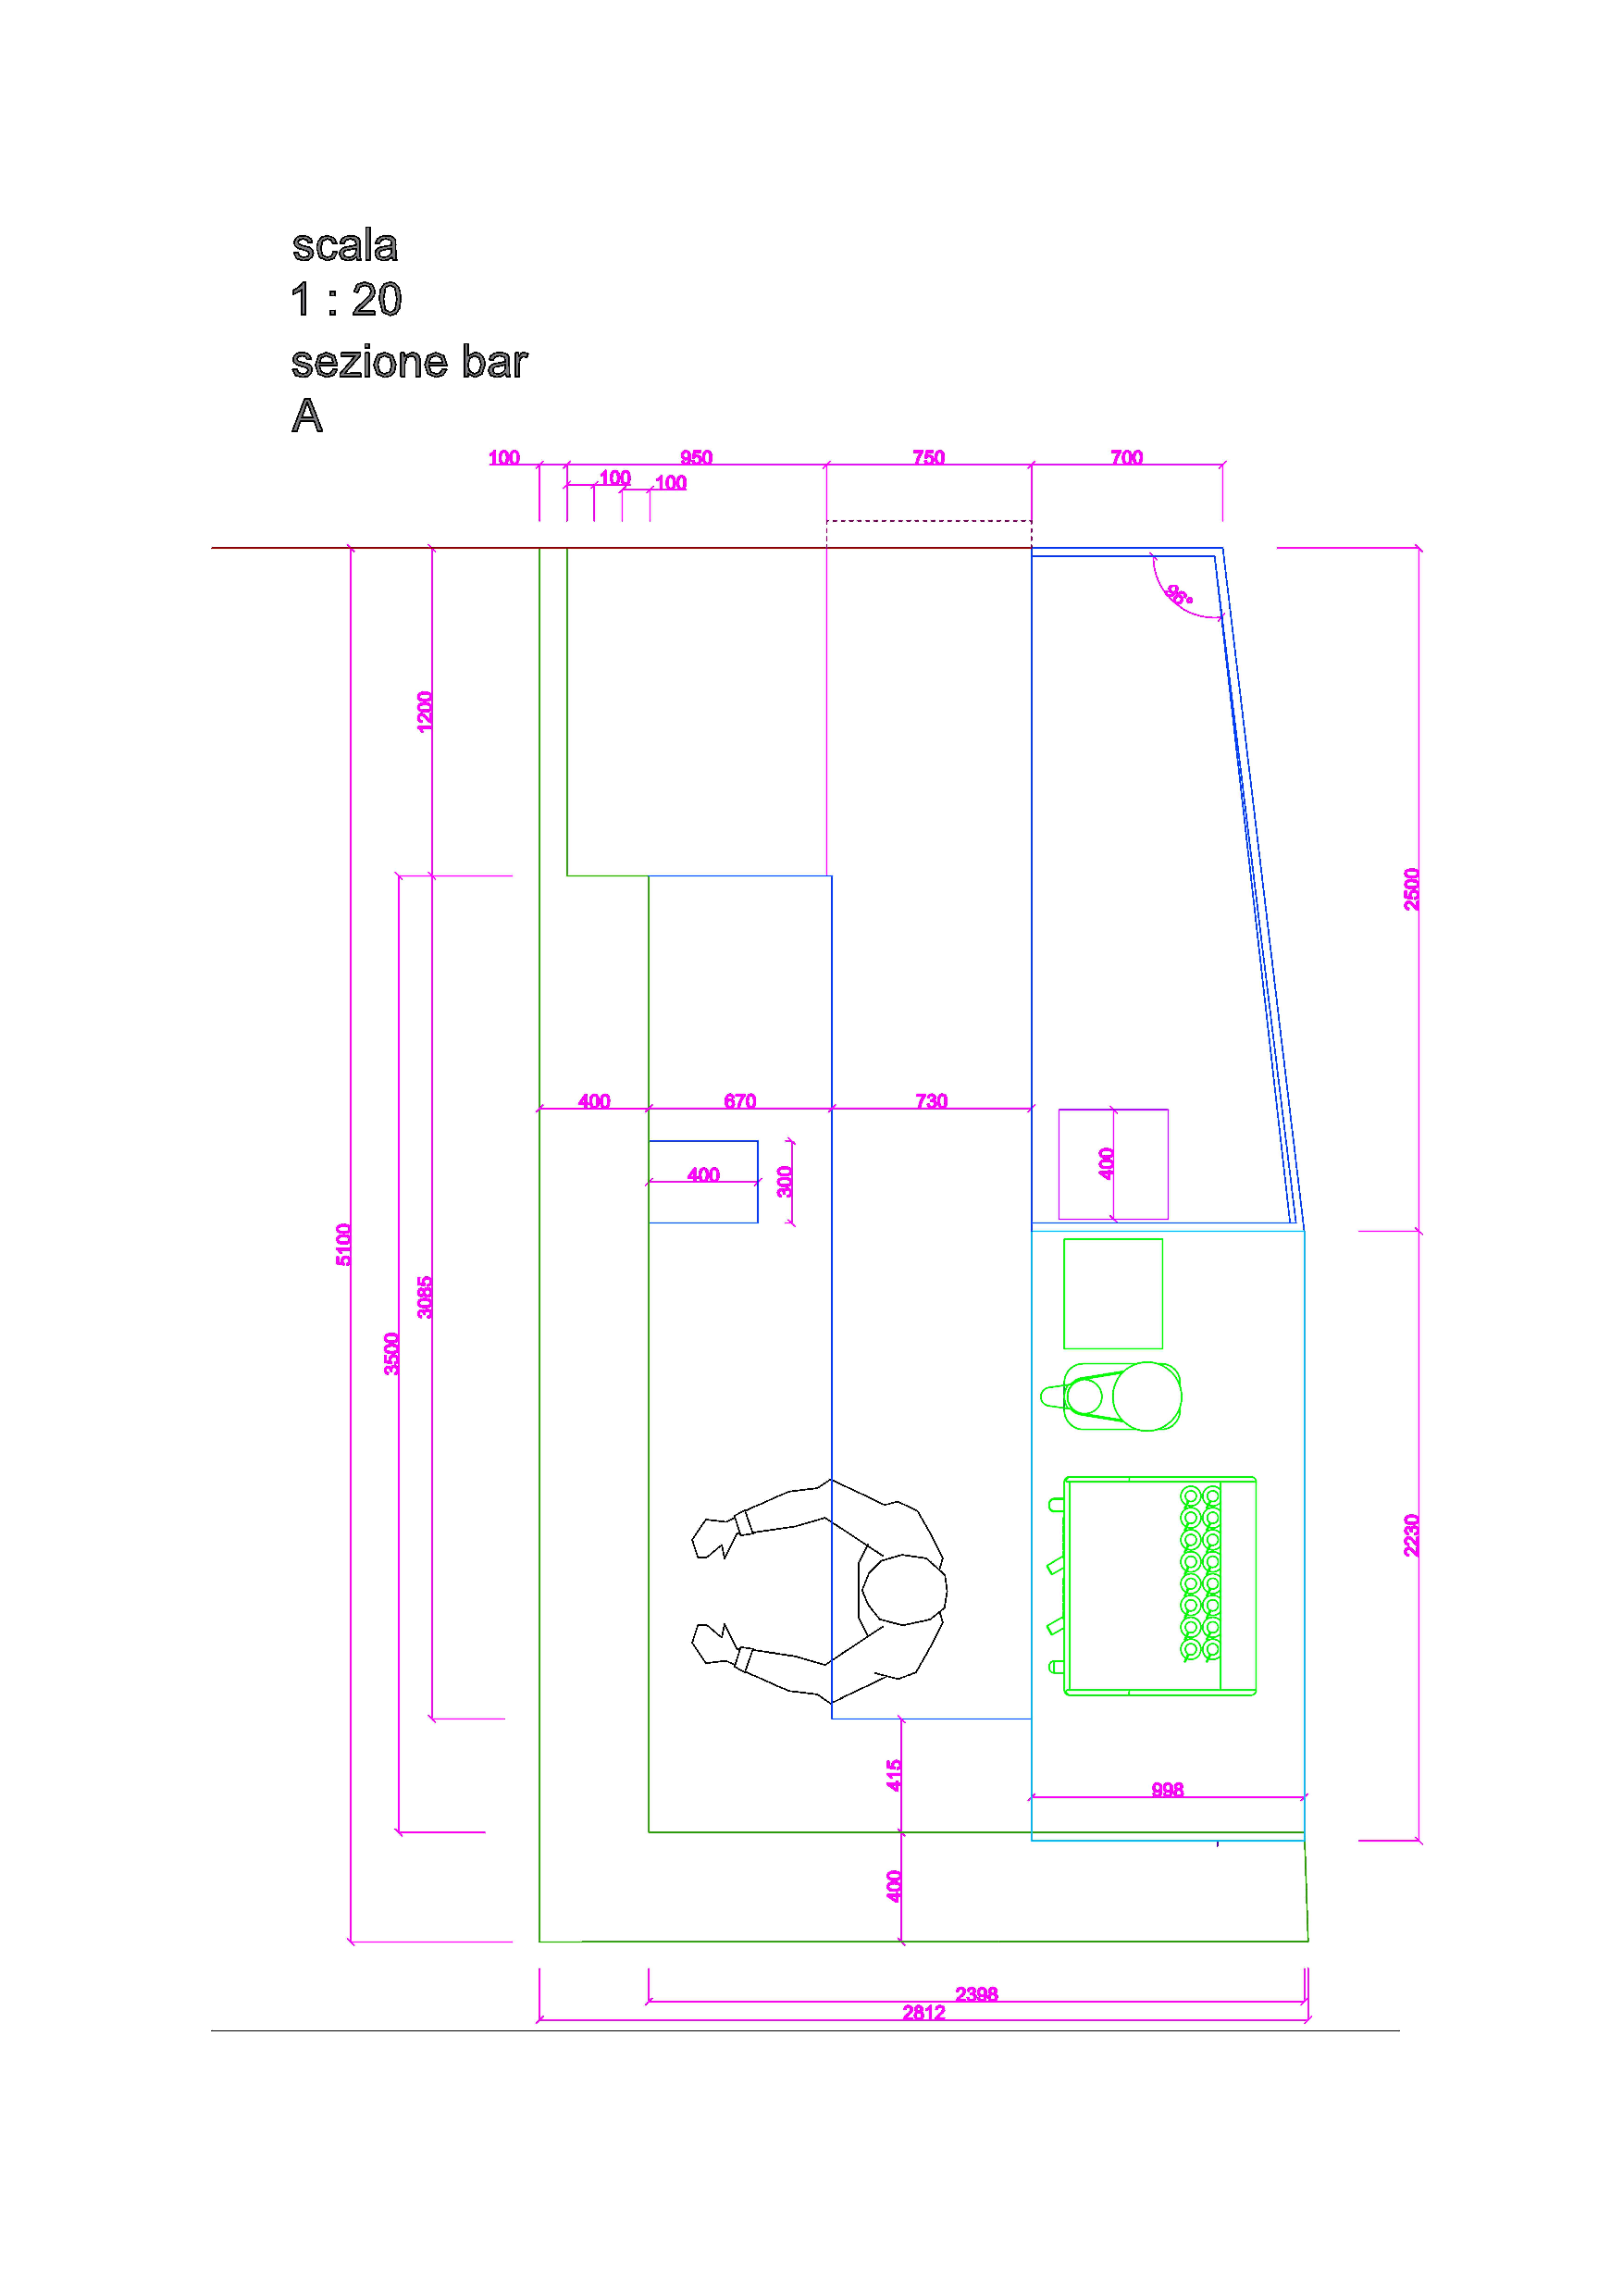
\includegraphics[width=1\linewidth]{13}
\end{figure}

\begin{figure}[H]
	\centering
	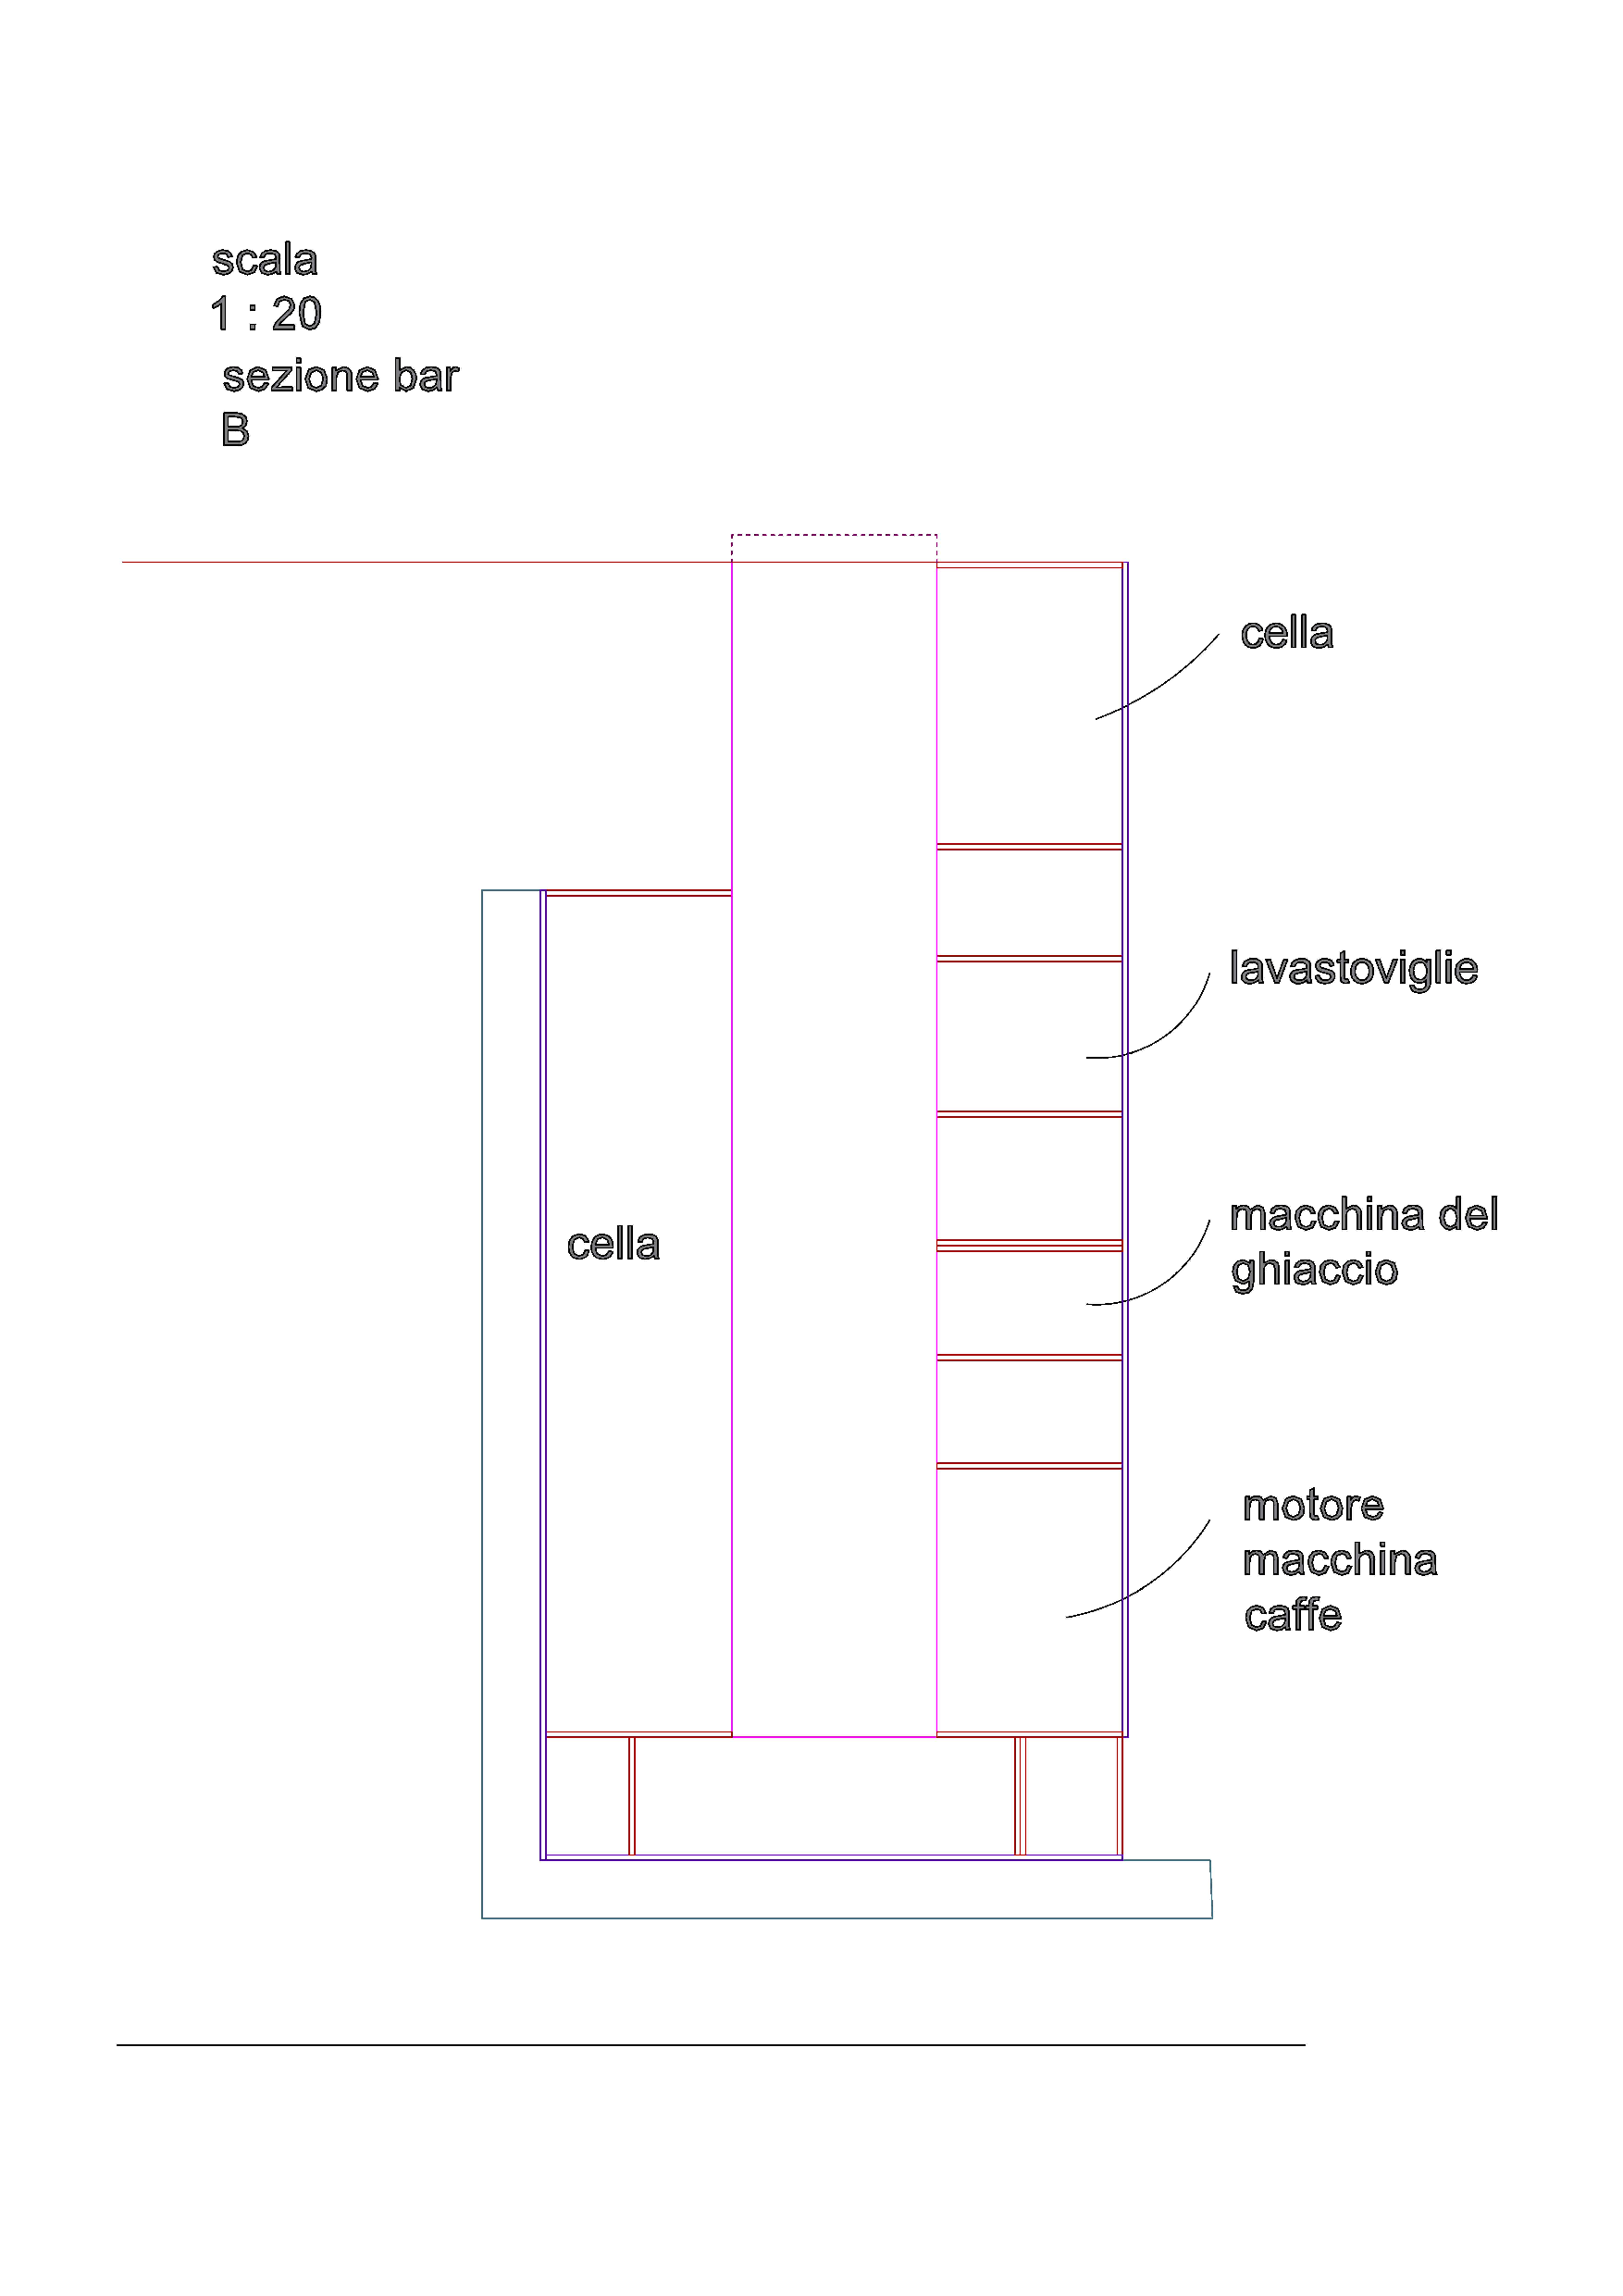
\includegraphics[width=1\linewidth]{14}
\end{figure}

\begin{figure}[H]
	\centering
	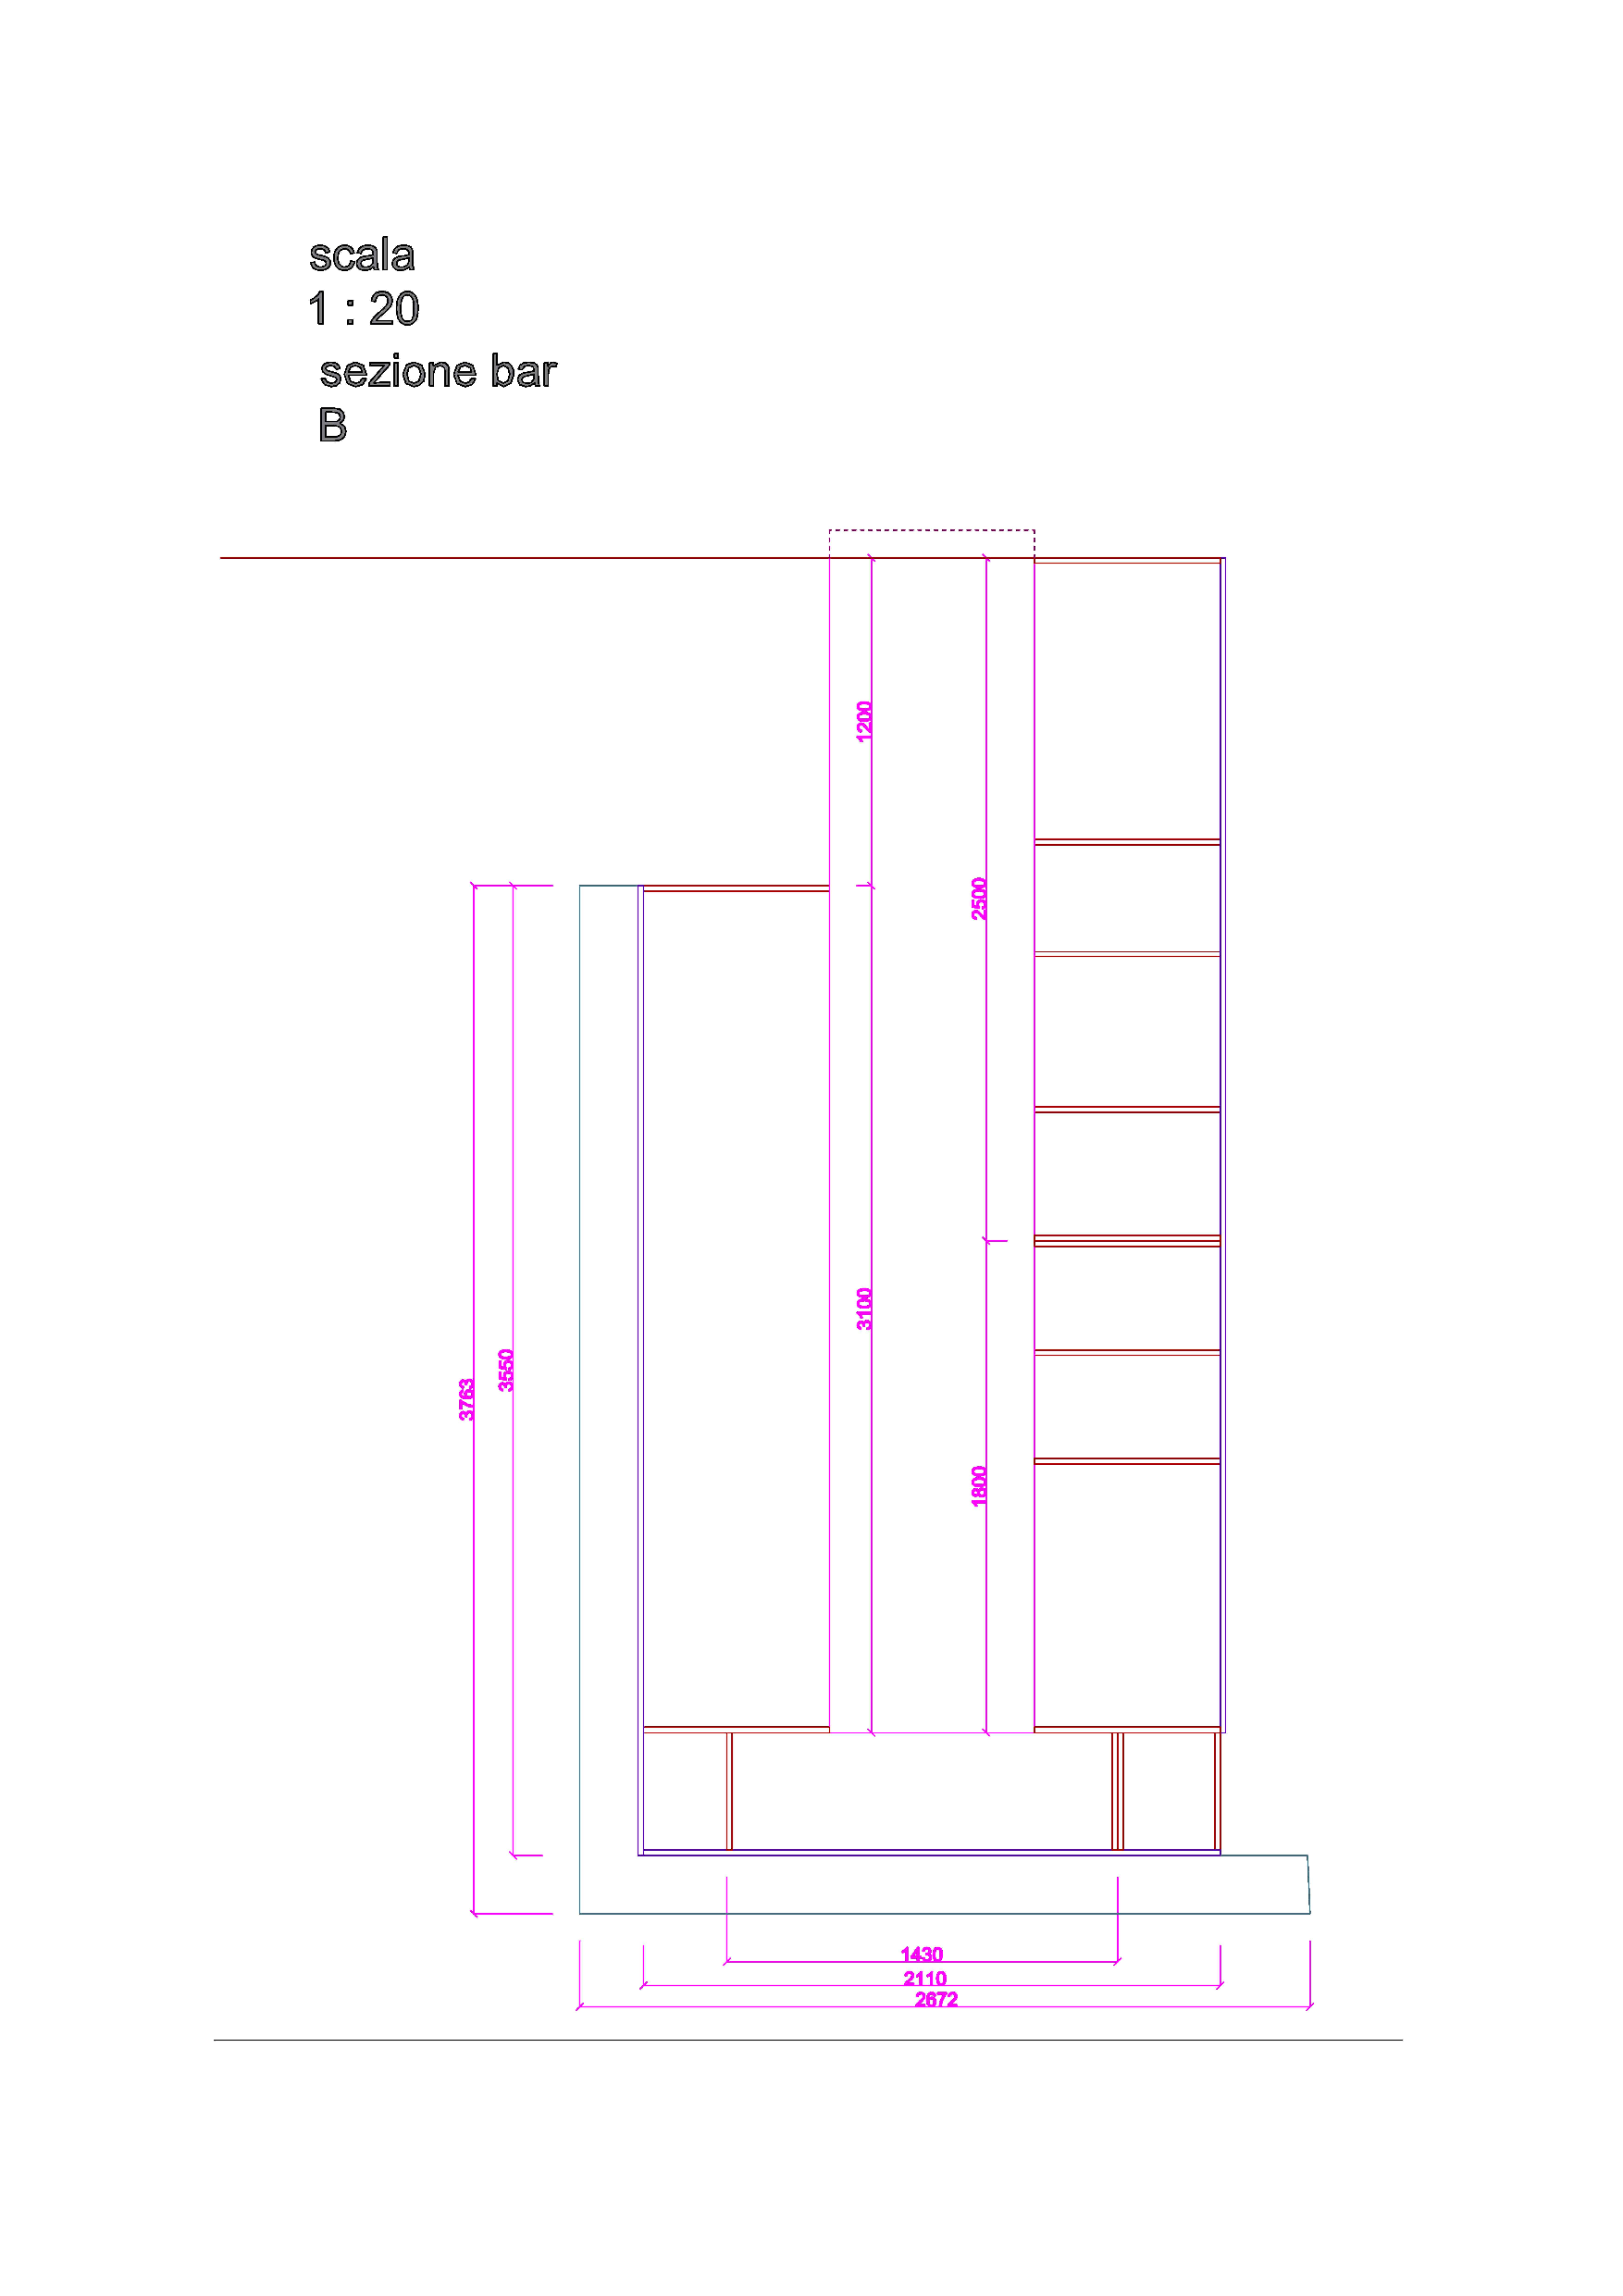
\includegraphics[width=1\linewidth]{15}
\end{figure}

\begin{figure}[H]
	\centering
	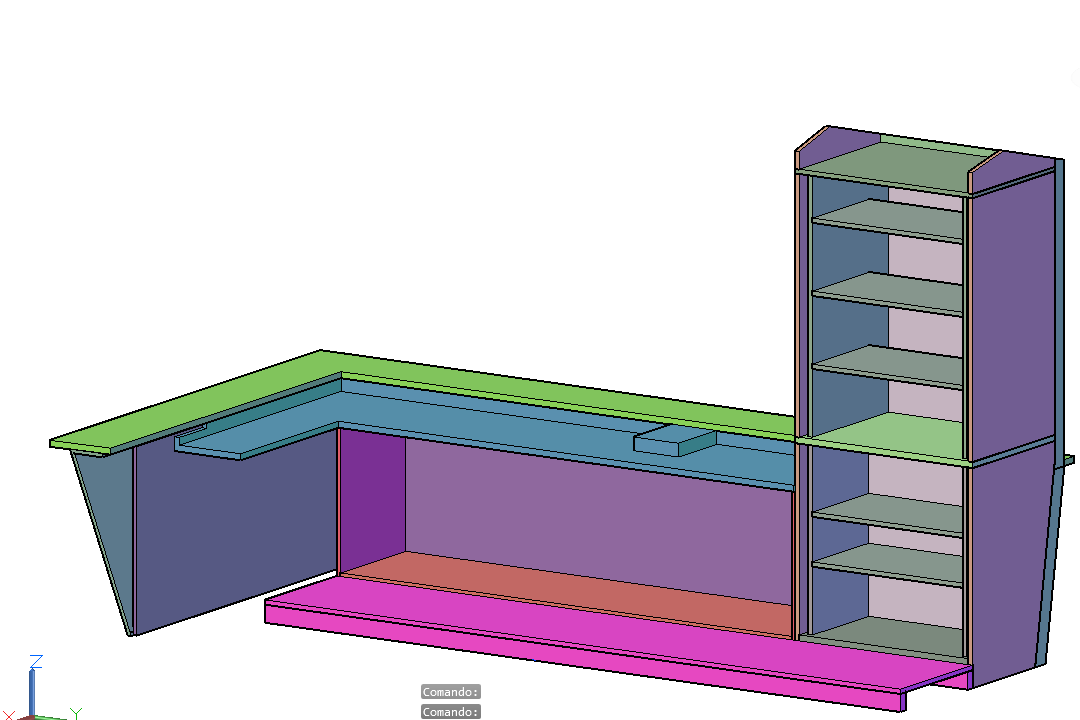
\includegraphics[width=0.8\linewidth]{16}
\end{figure}

\newpage
\begin{figure}[H]
	\centering
	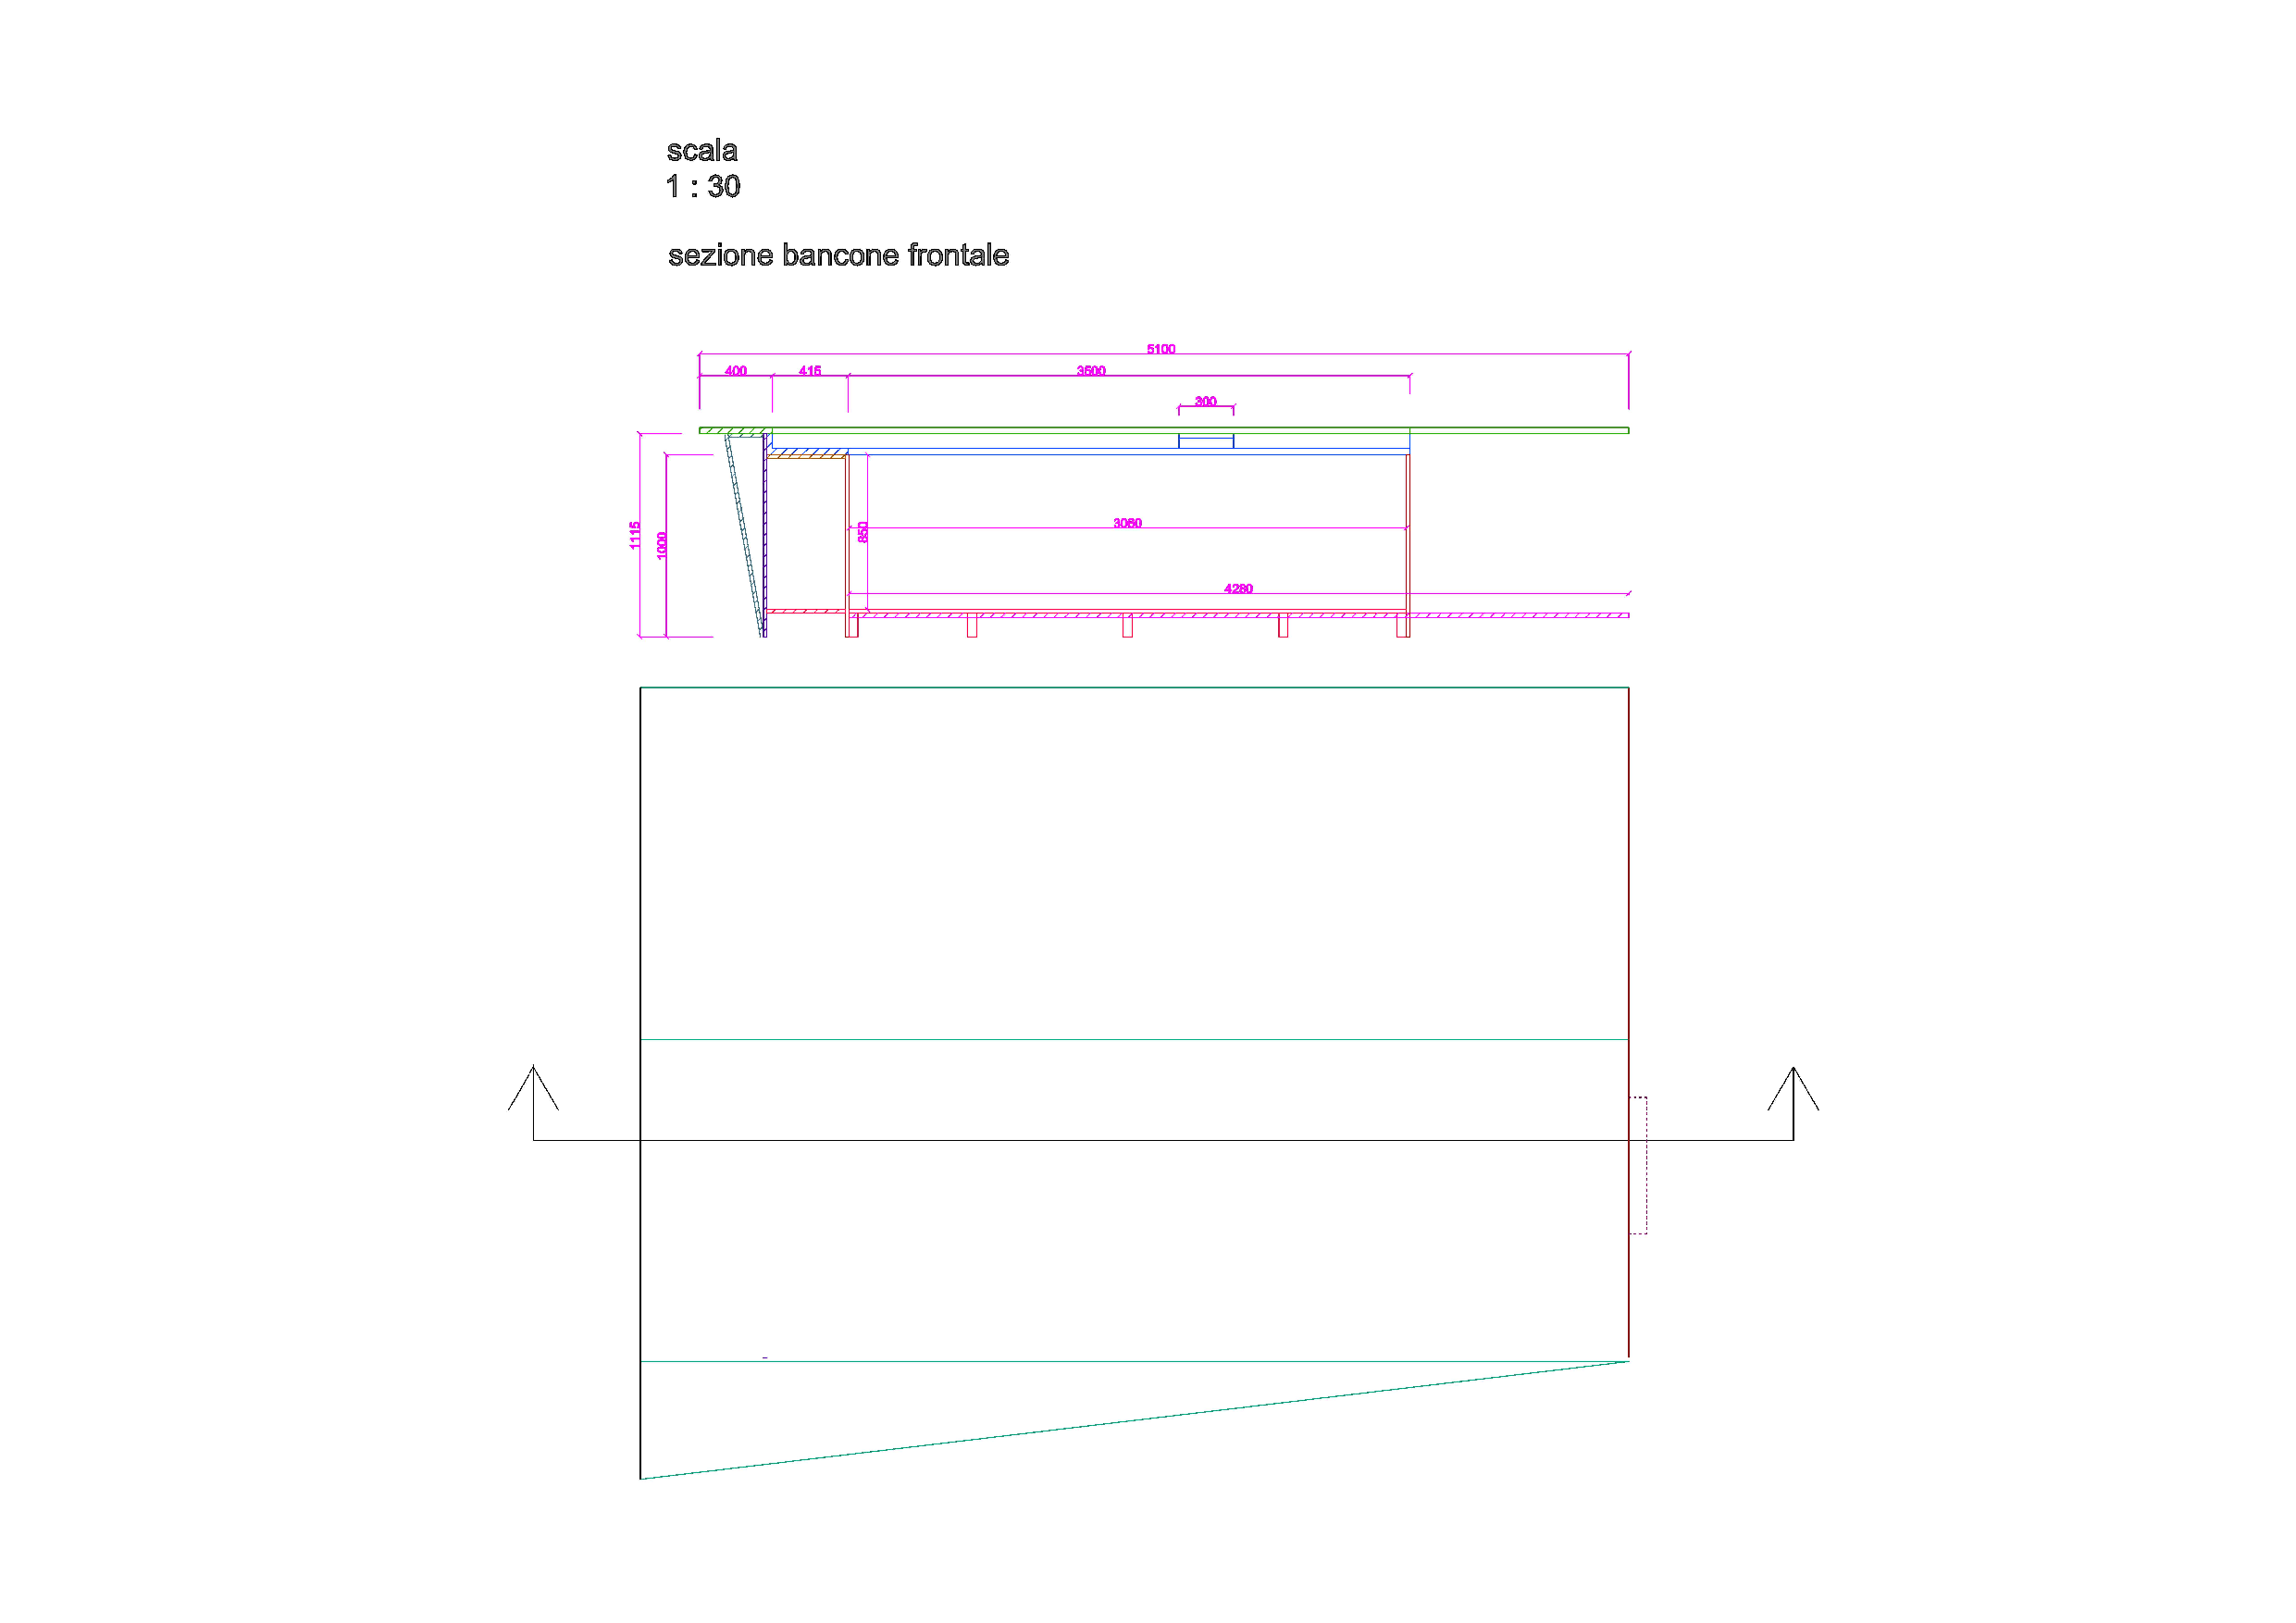
\includegraphics[width=1\linewidth]{17}
\end{figure}

\newpage
\begin{figure}[H]
	\centering
	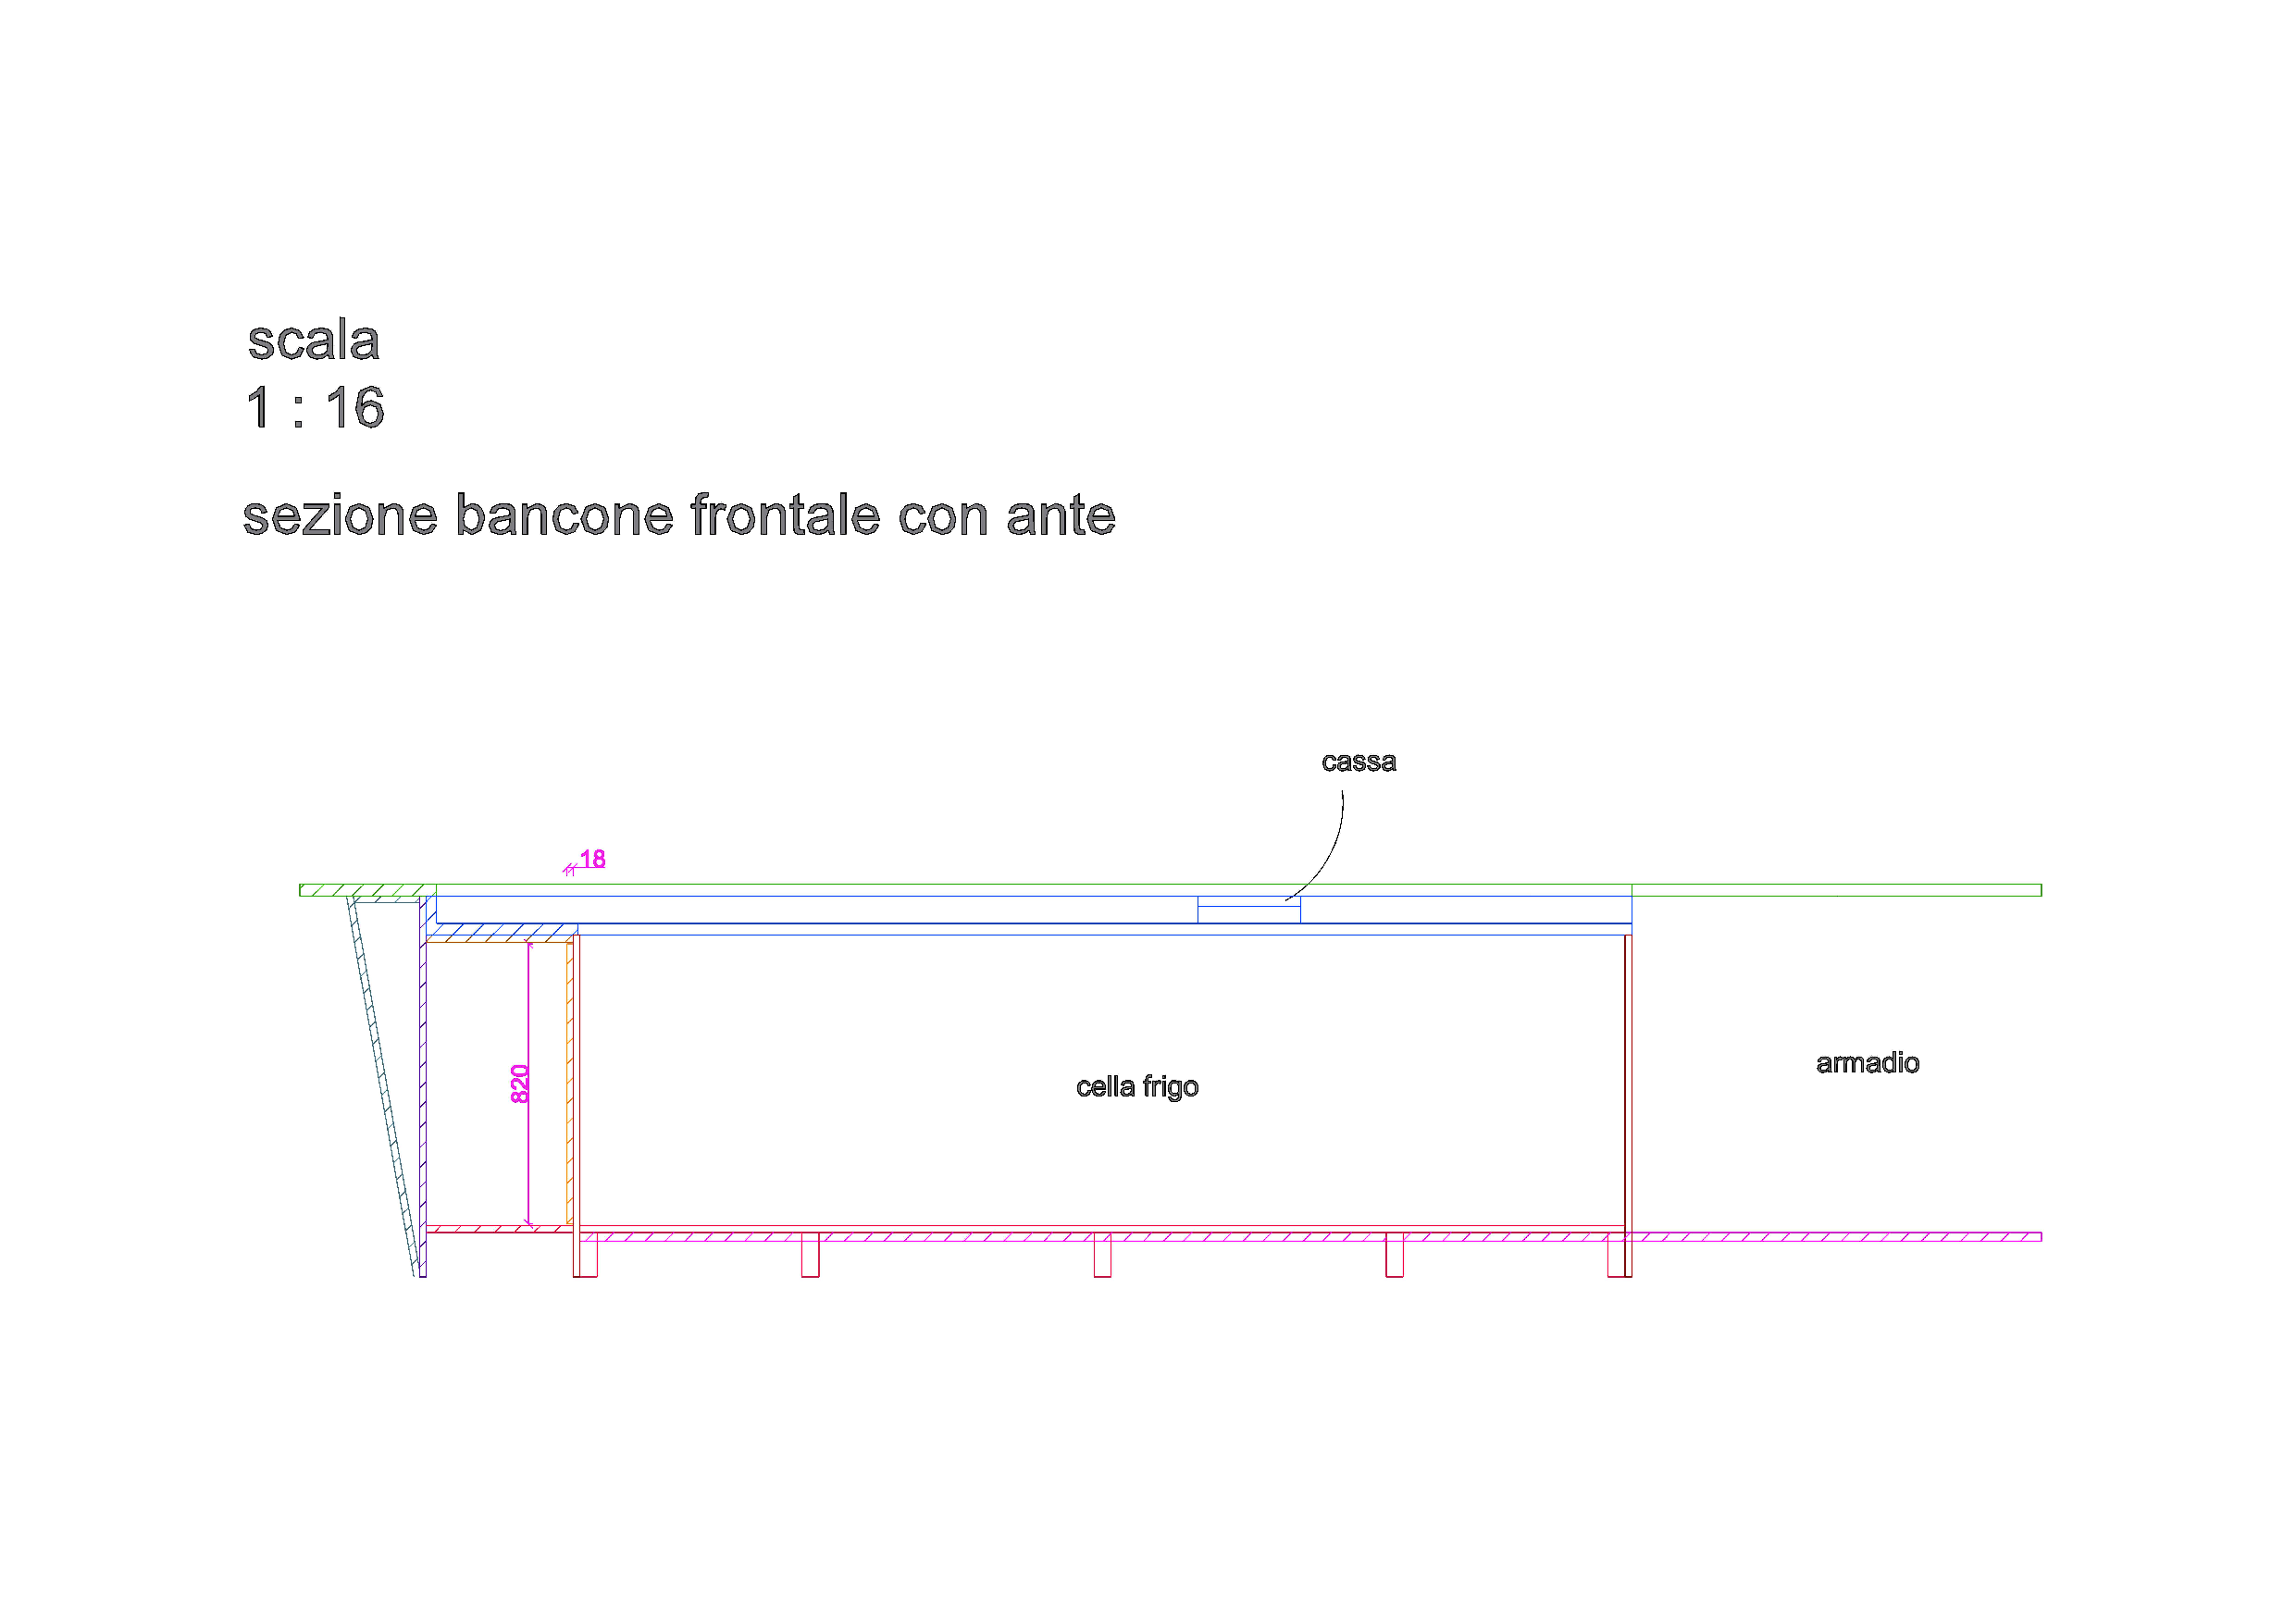
\includegraphics[width=0.8\linewidth]{18}
\end{figure}

\begin{figure}[H]
	\centering
	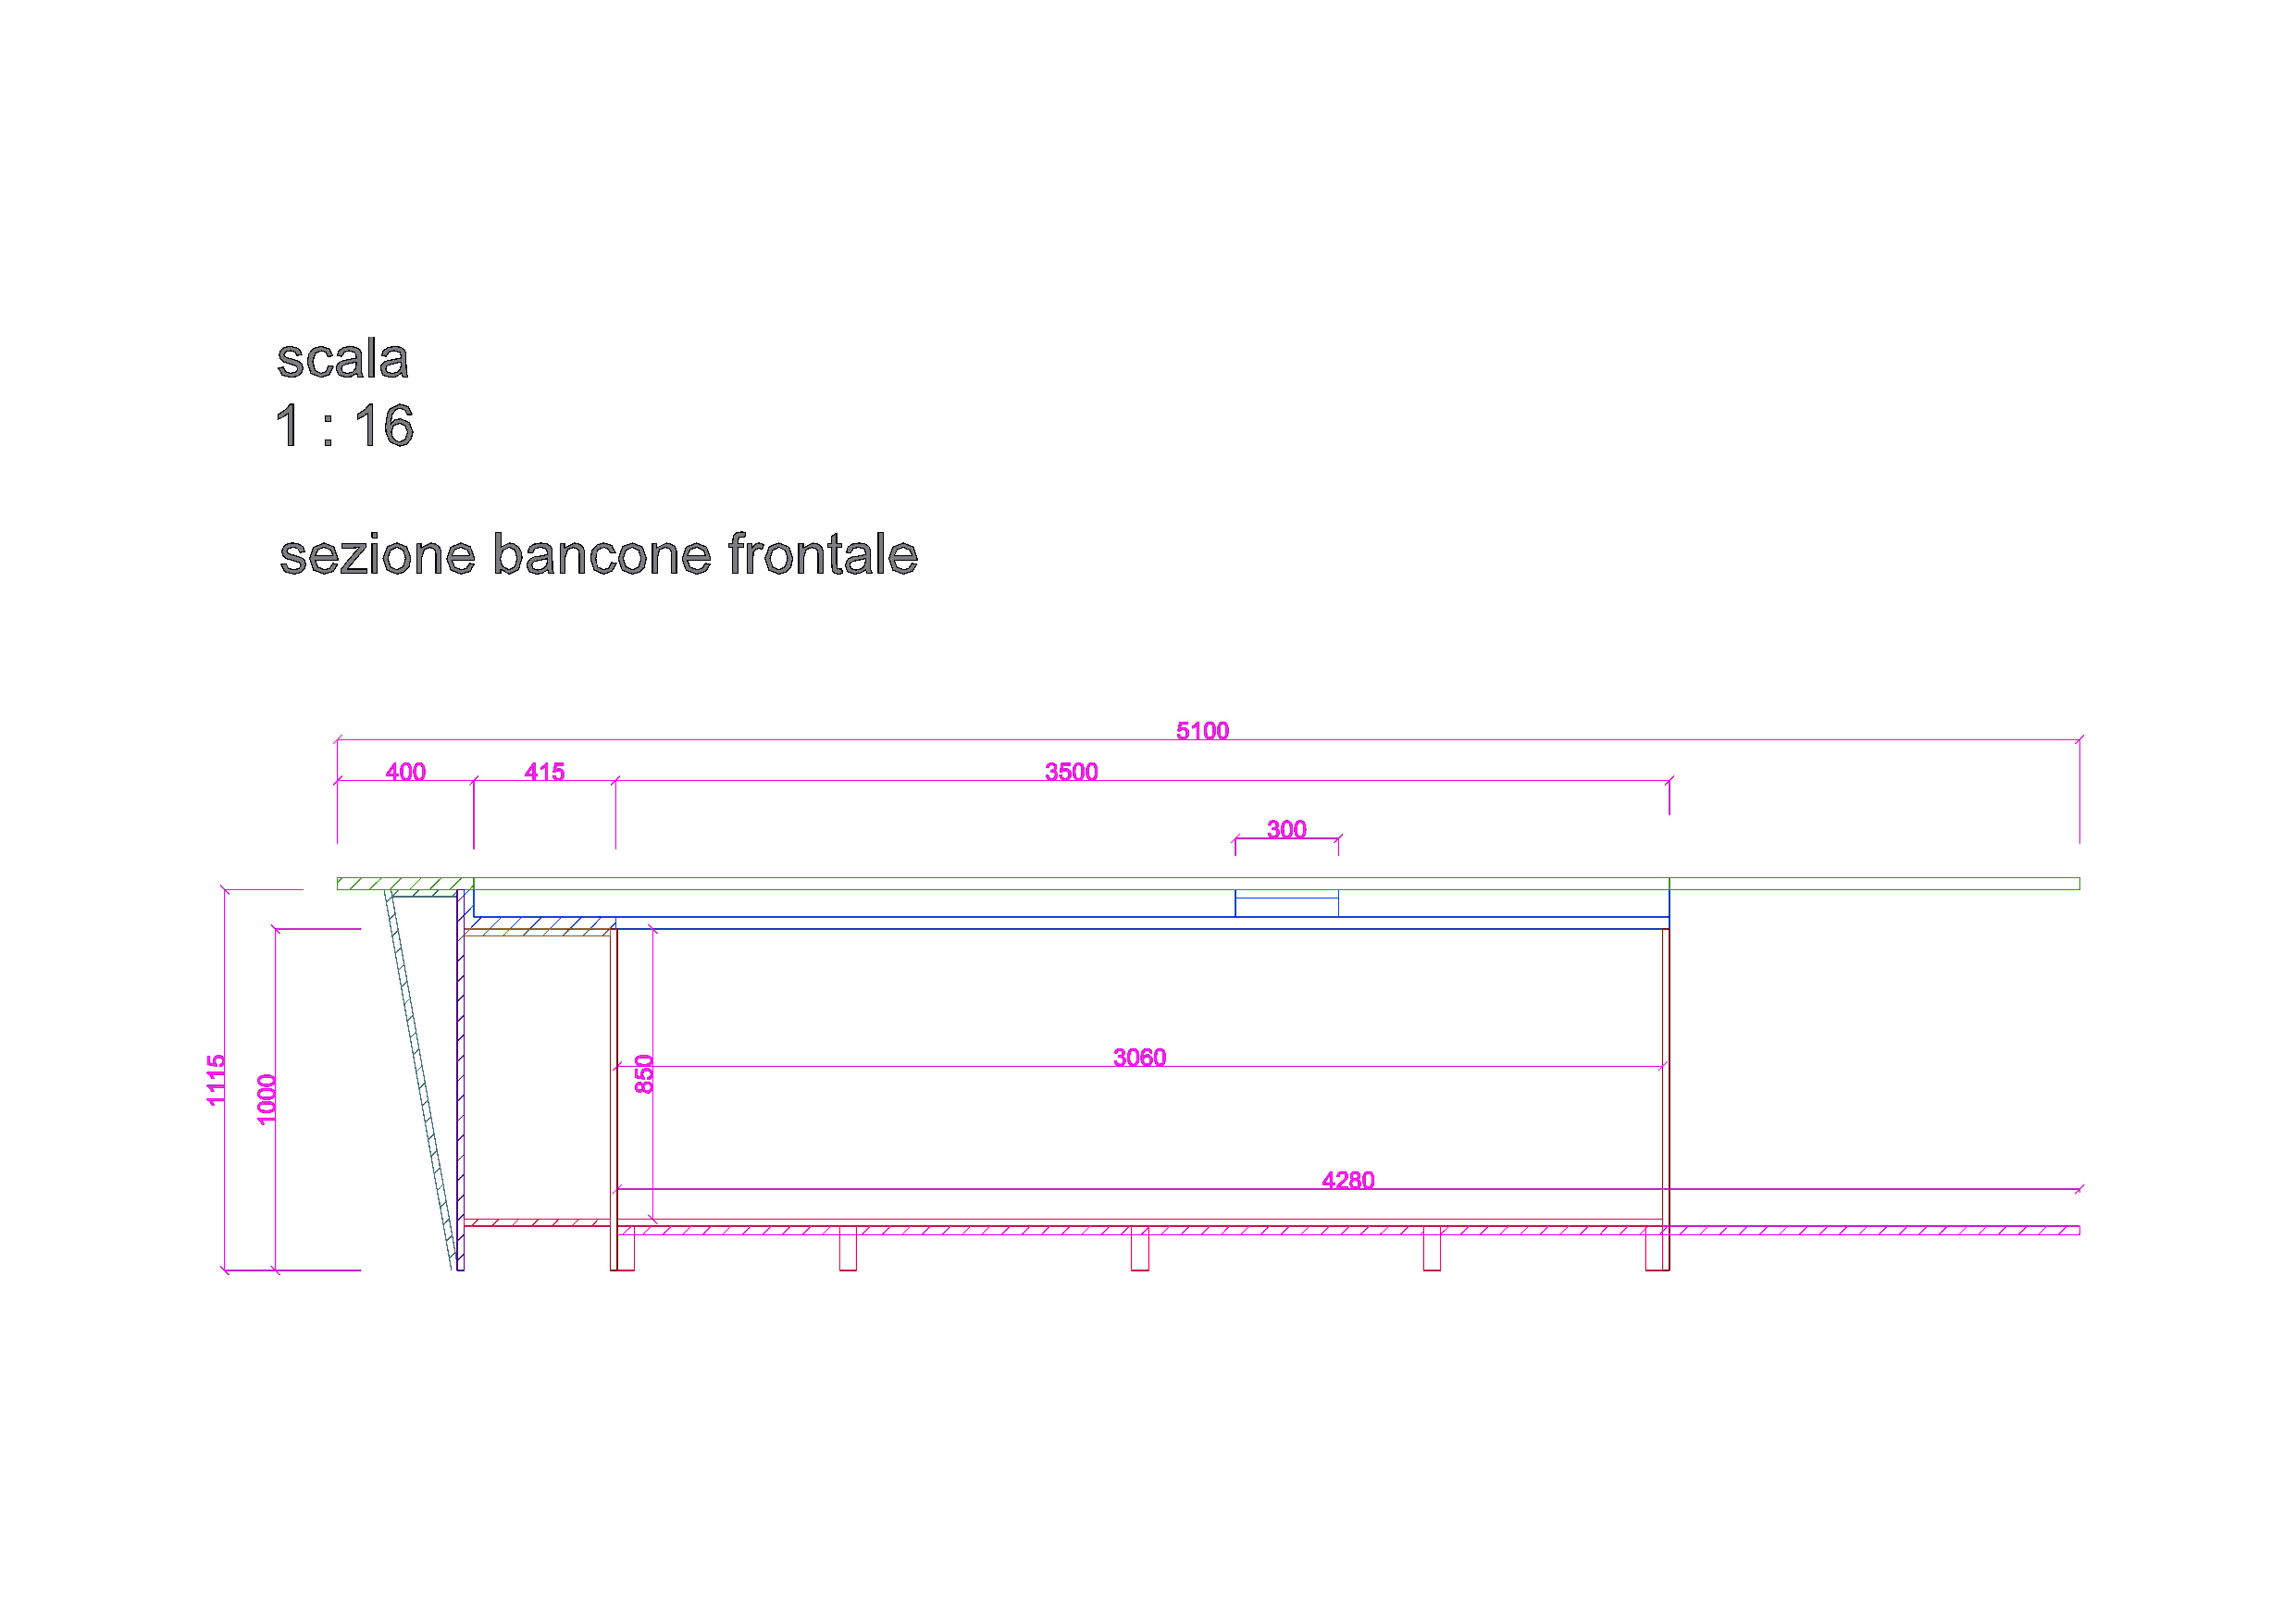
\includegraphics[width=0.8\linewidth]{19}
\end{figure}

\clearpage
\begin{figure}[H]
	\centering
	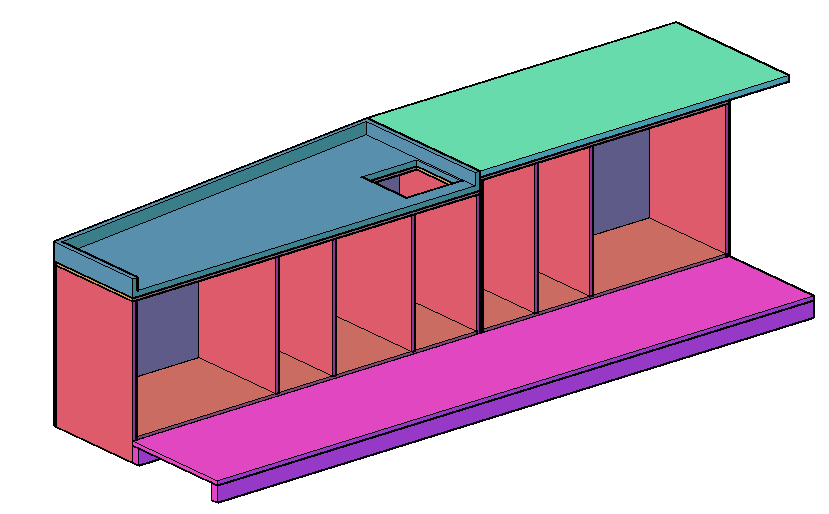
\includegraphics[width=1\linewidth]{20}
\end{figure}

% ---------------------------------------
\newpage
\begin{figure}[H]
	\centering
	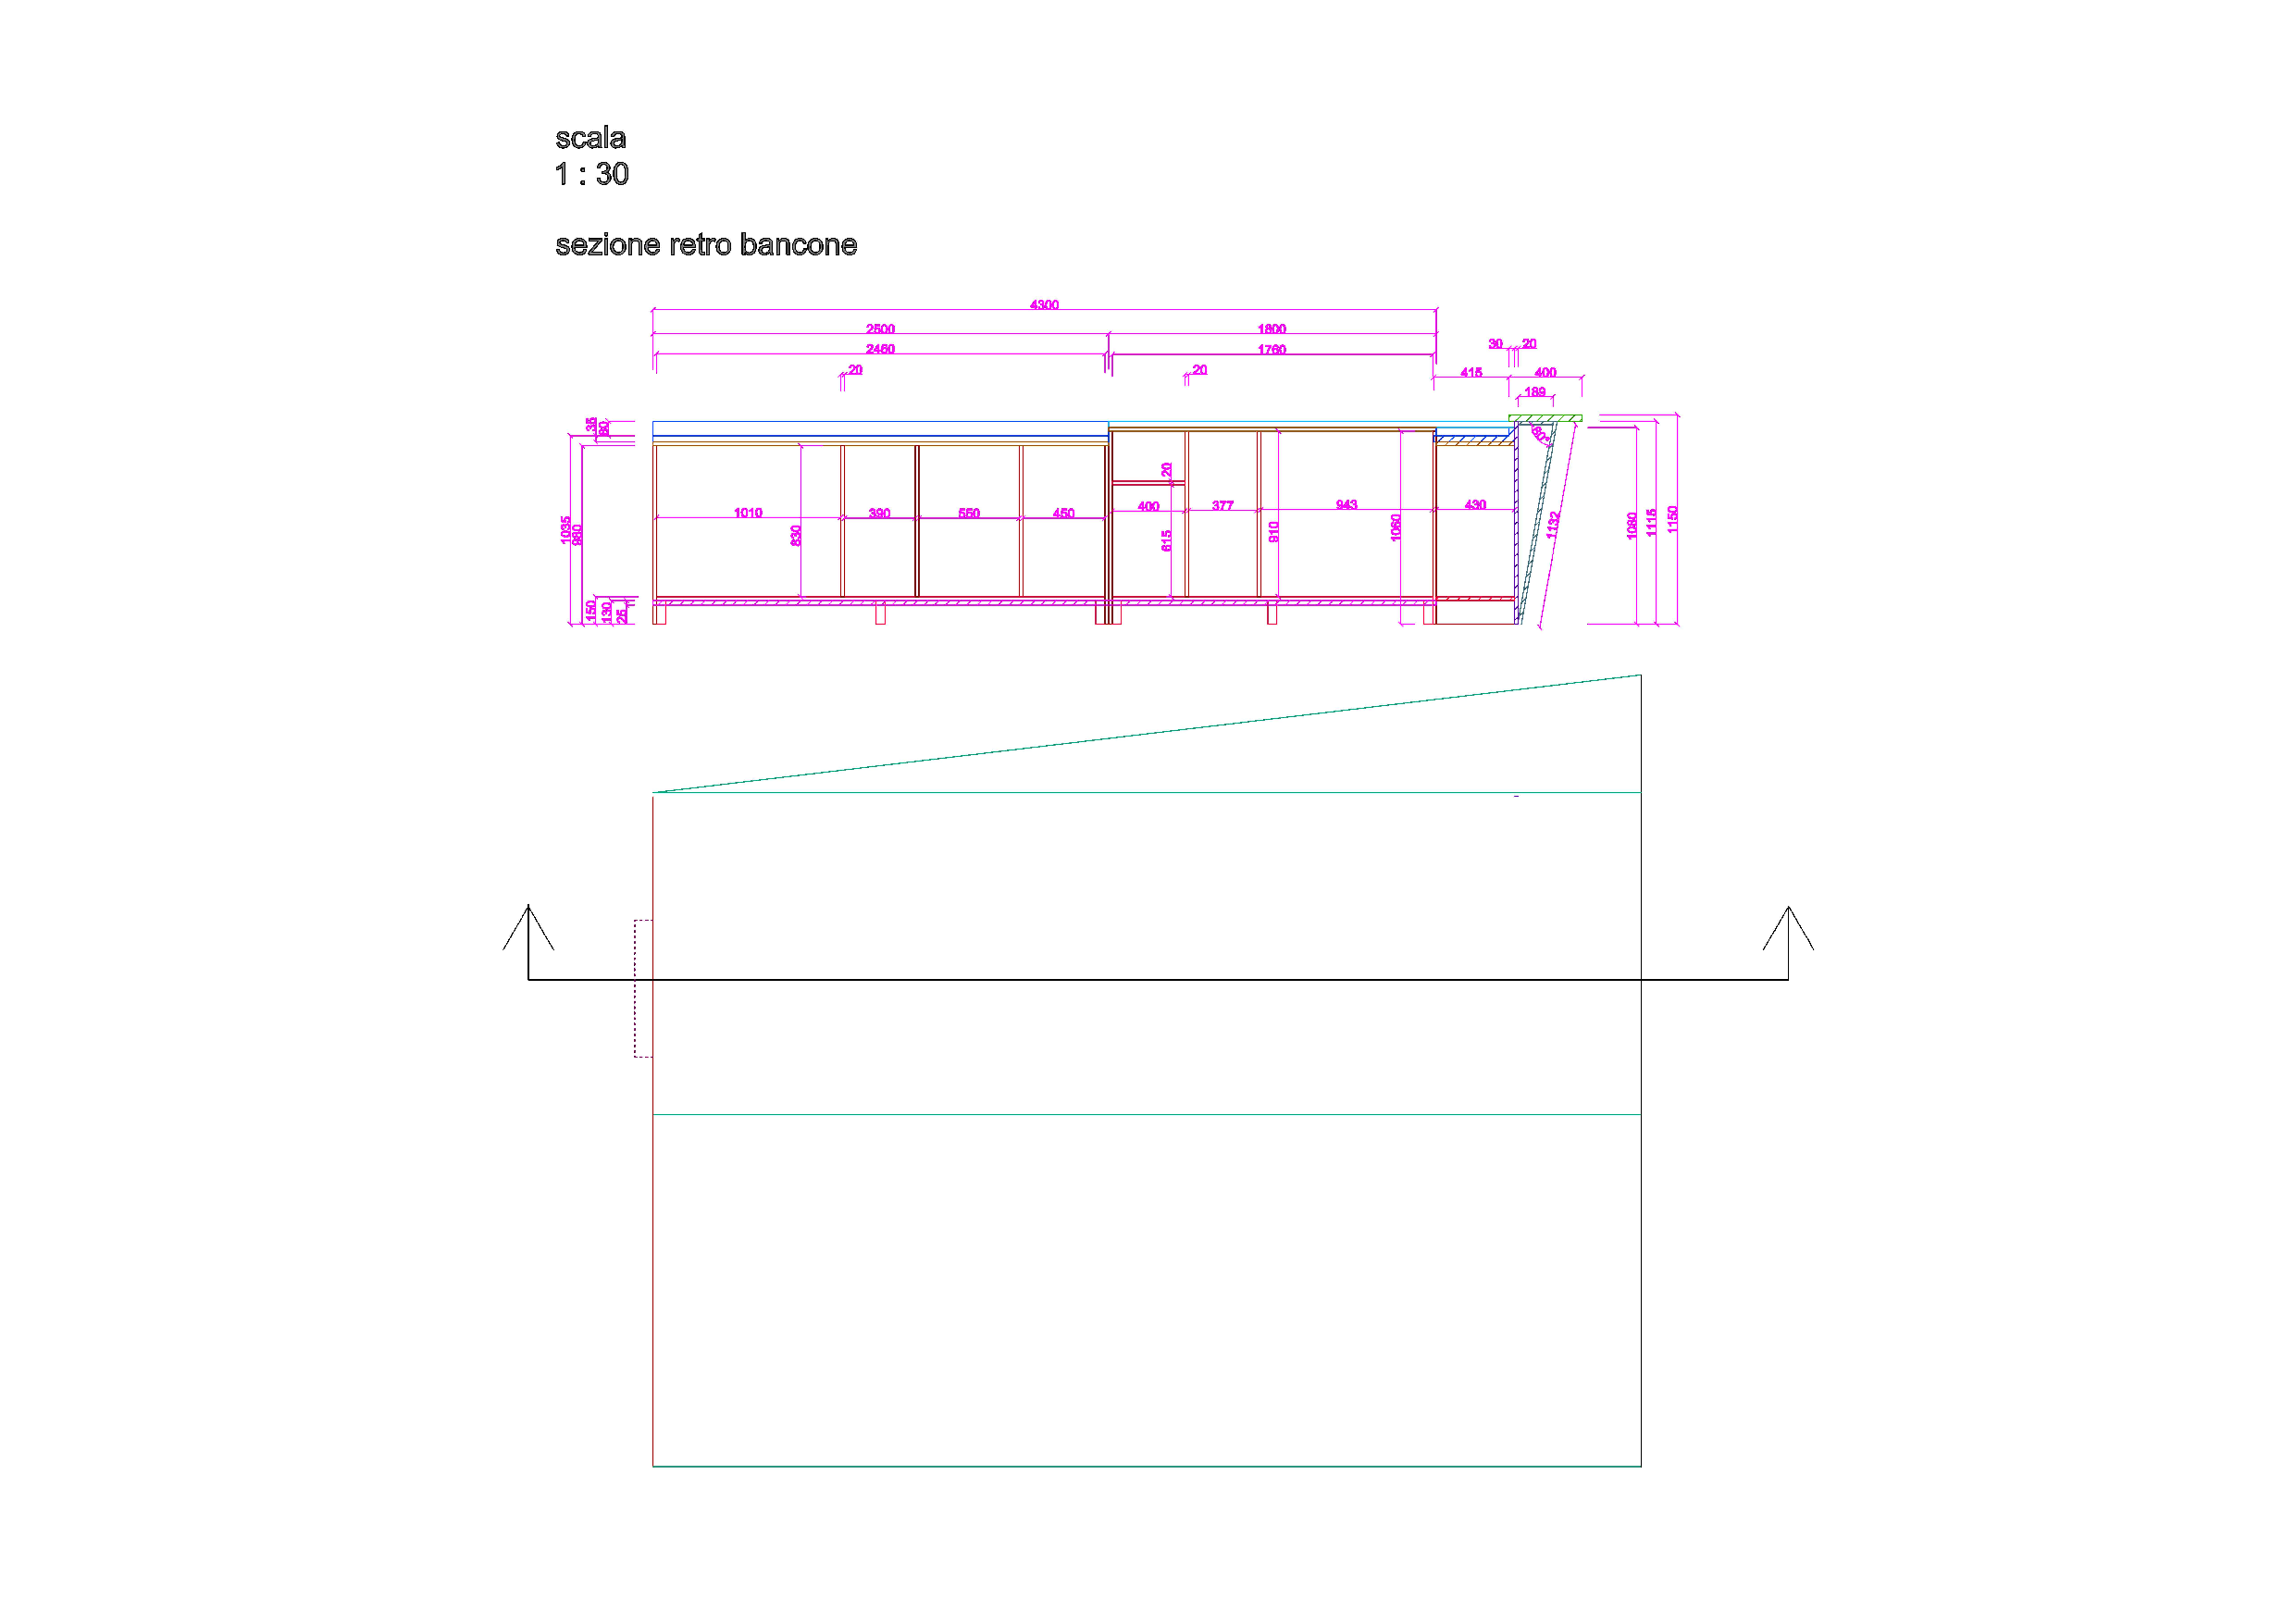
\includegraphics[width=1\linewidth]{21}
\end{figure}

\newpage
\begin{figure}[H]
	\centering
	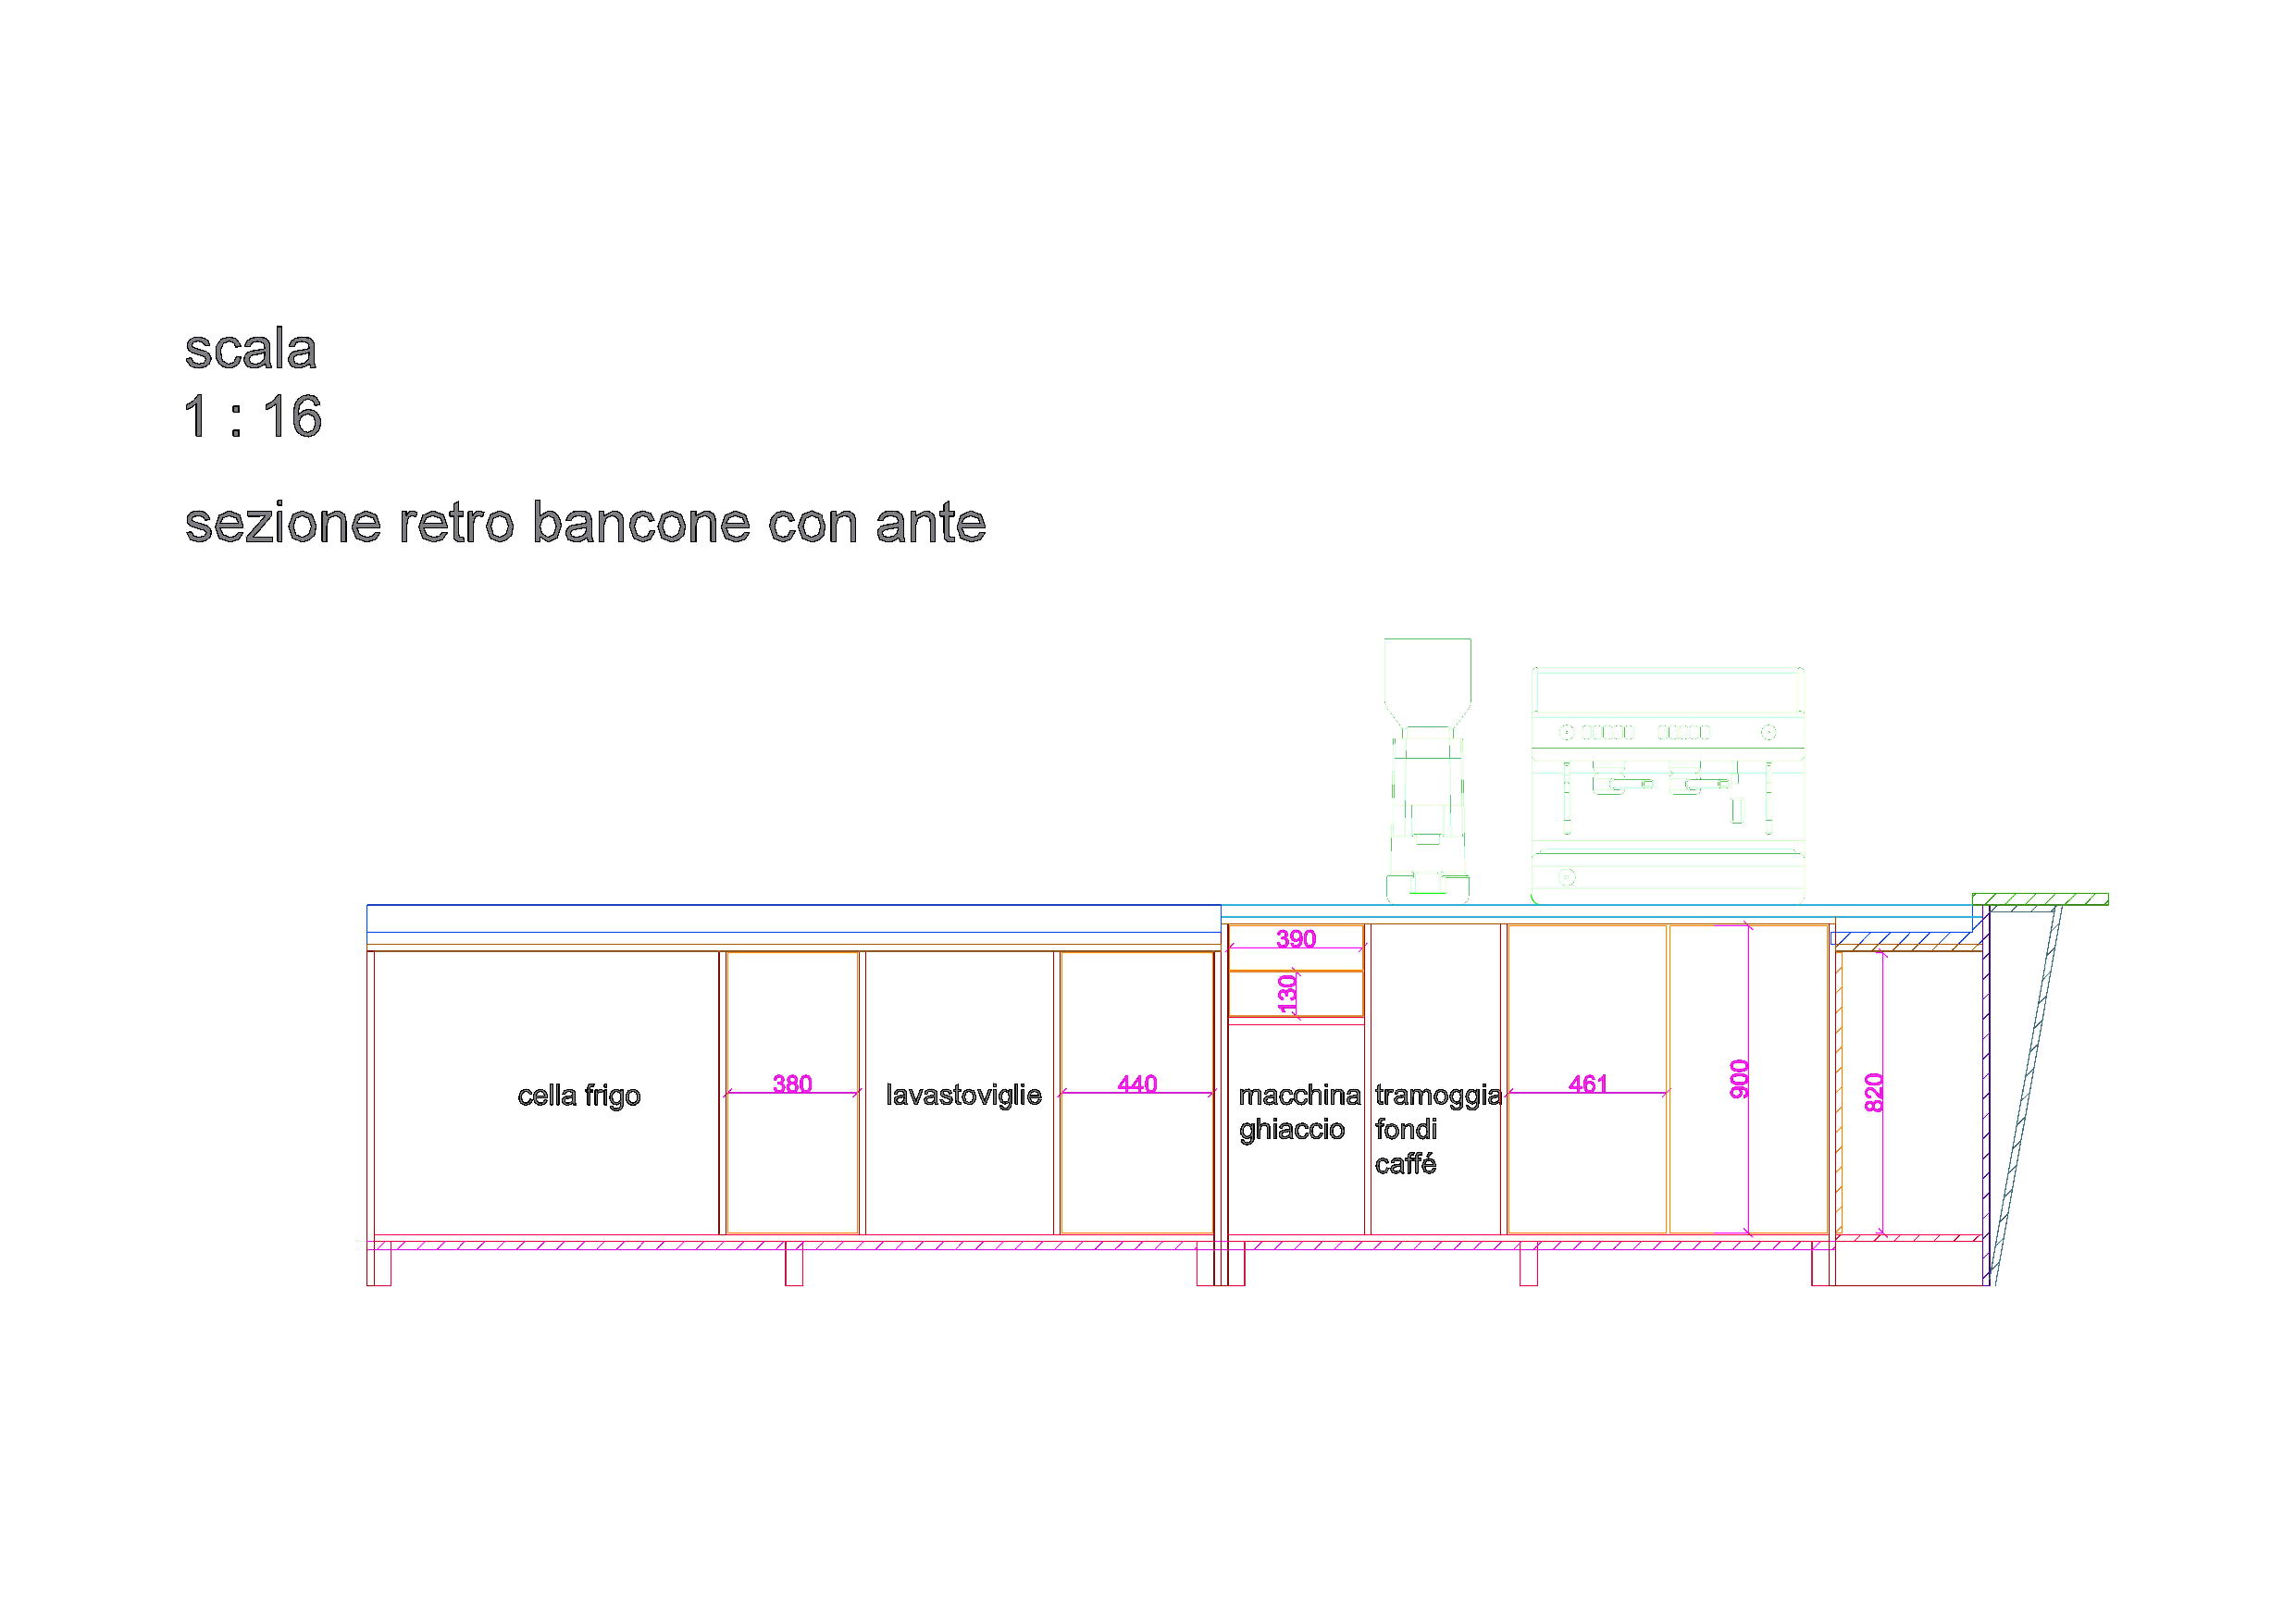
\includegraphics[width=.9\linewidth]{22}
\end{figure}

\begin{figure}[H]
	\centering
	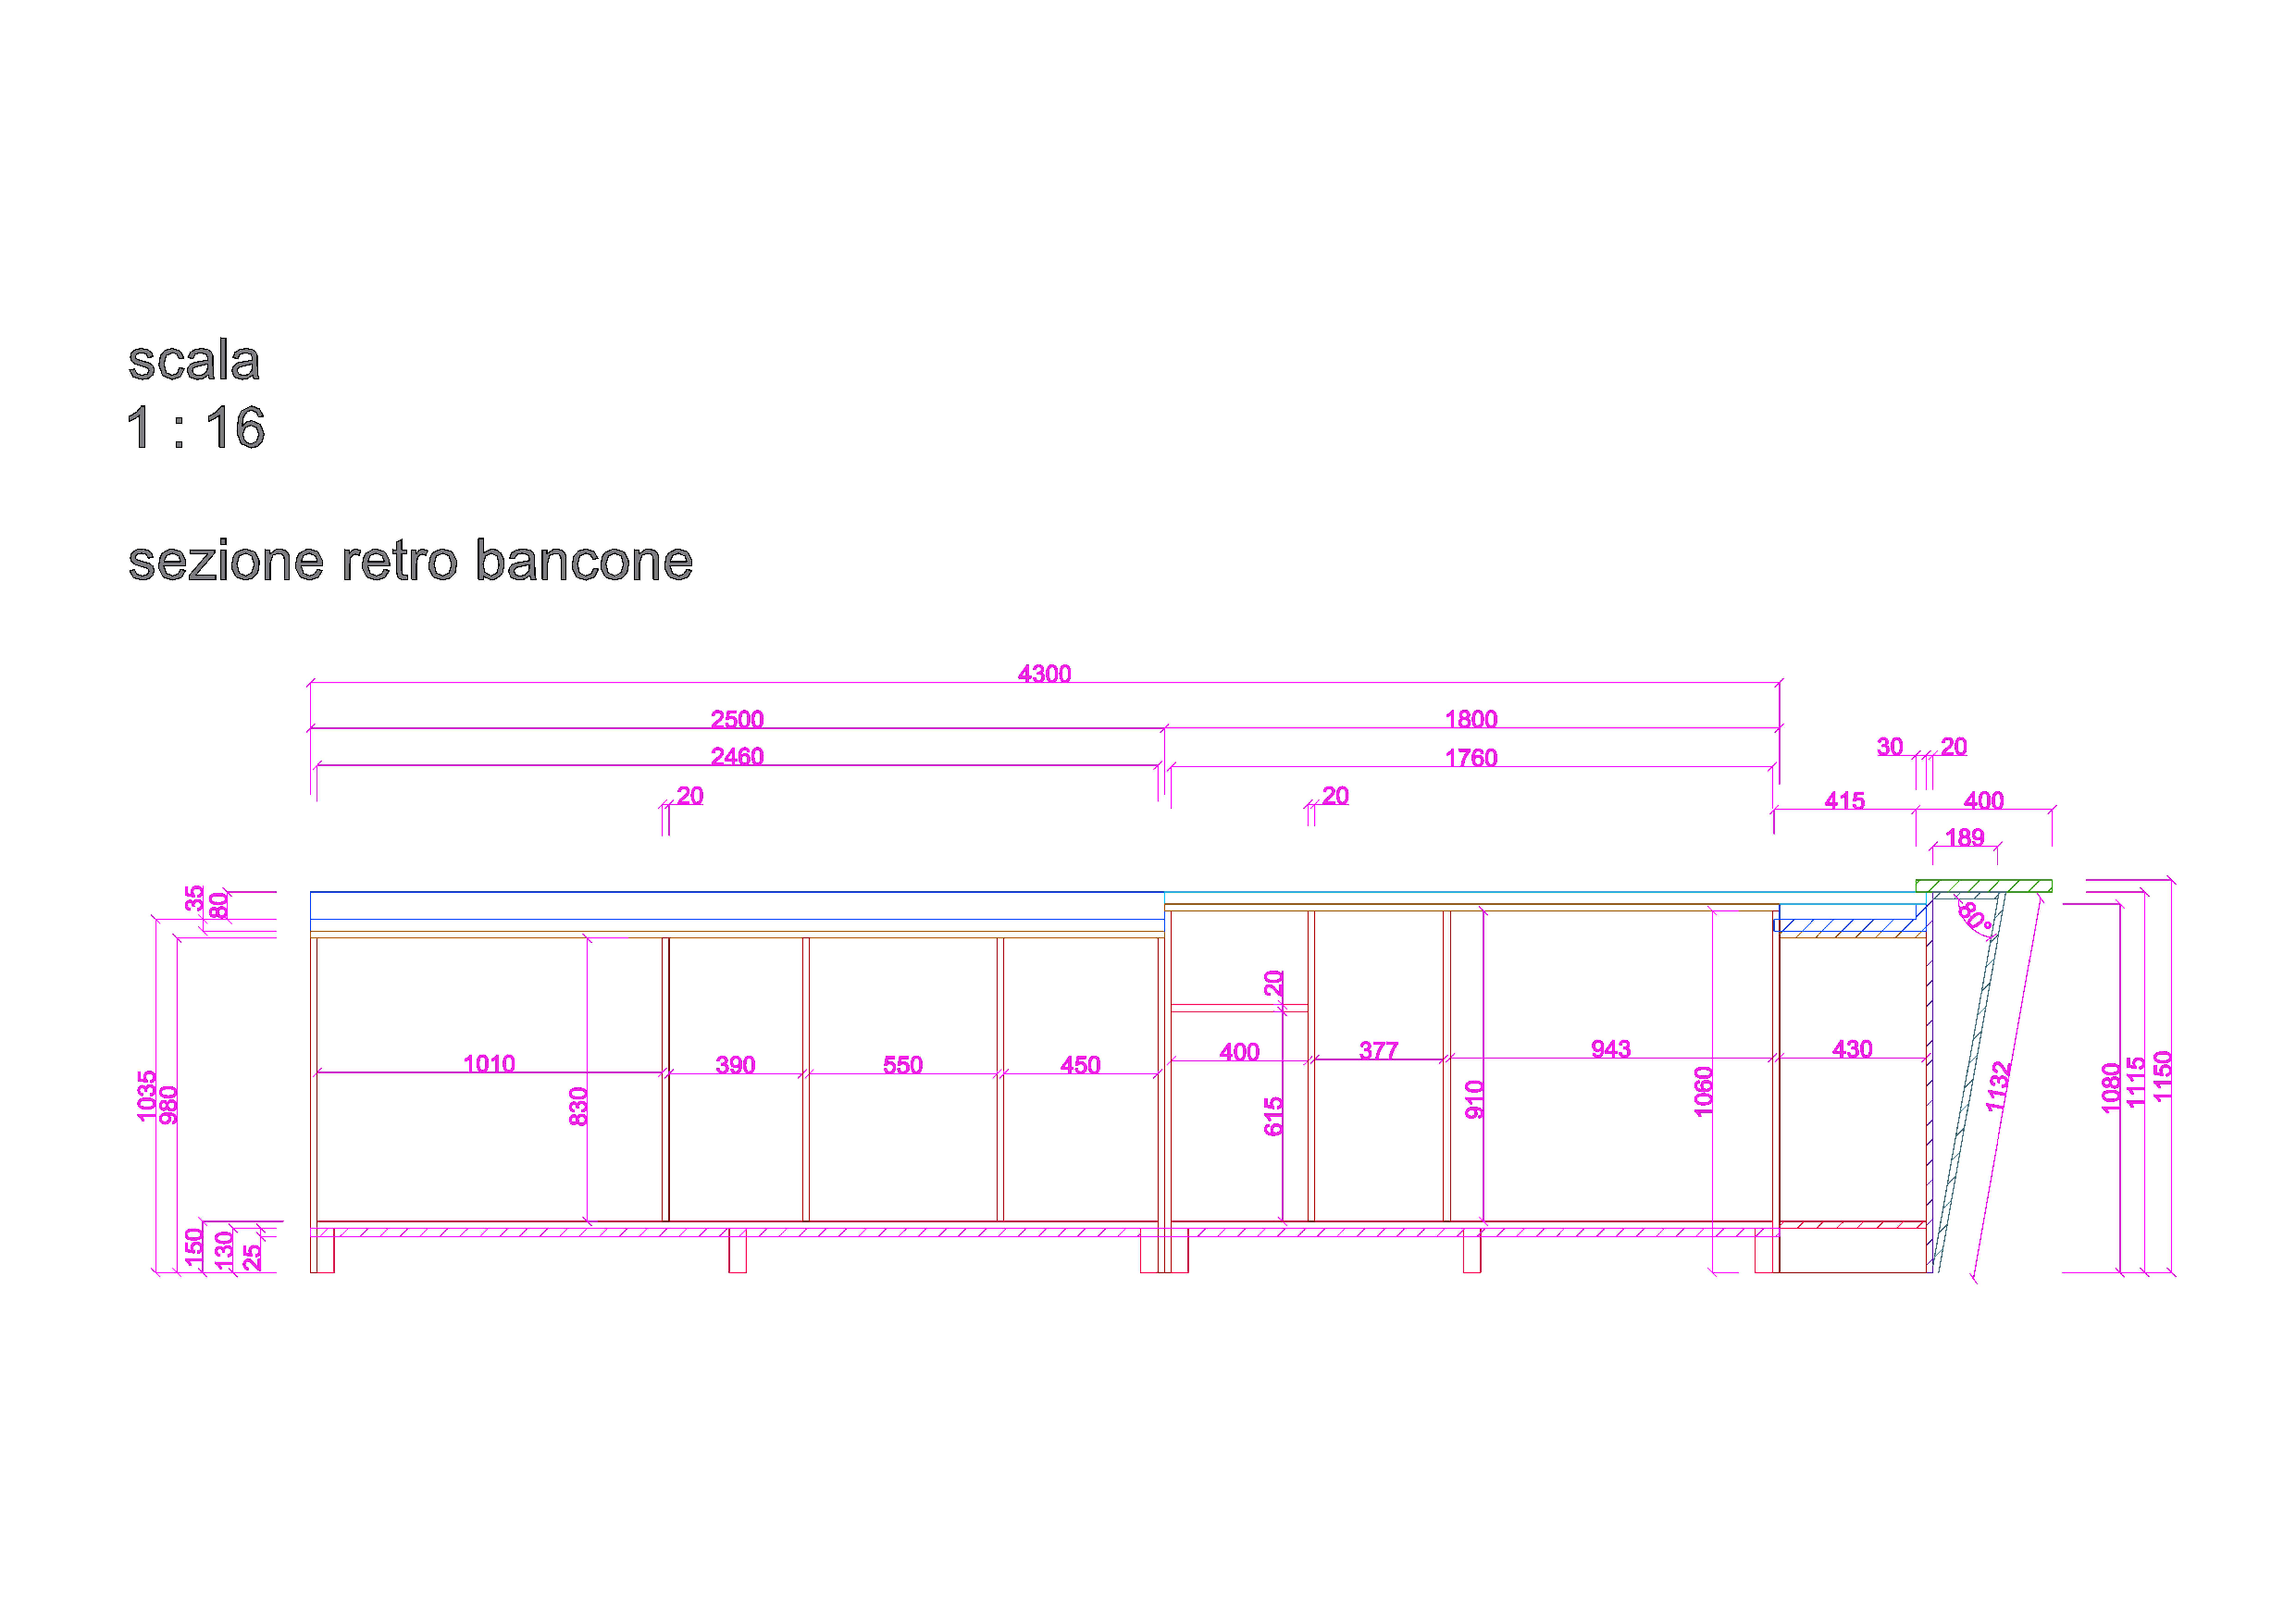
\includegraphics[width=.9\linewidth]{23}
\end{figure}

\begin{figure}[H]
	\centering
	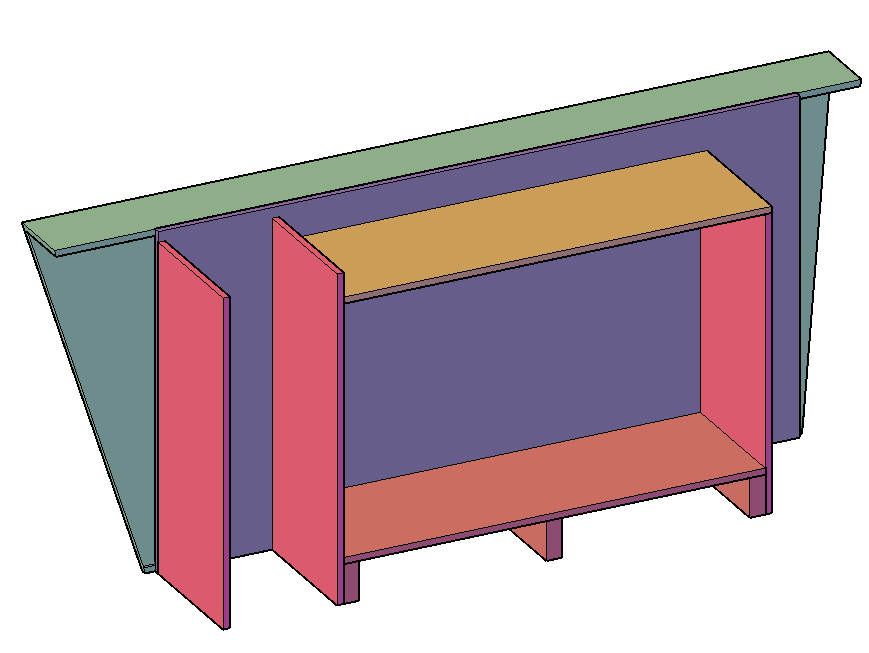
\includegraphics[width=1\linewidth]{24}
\end{figure}

\begin{figure}[H]
	\centering
	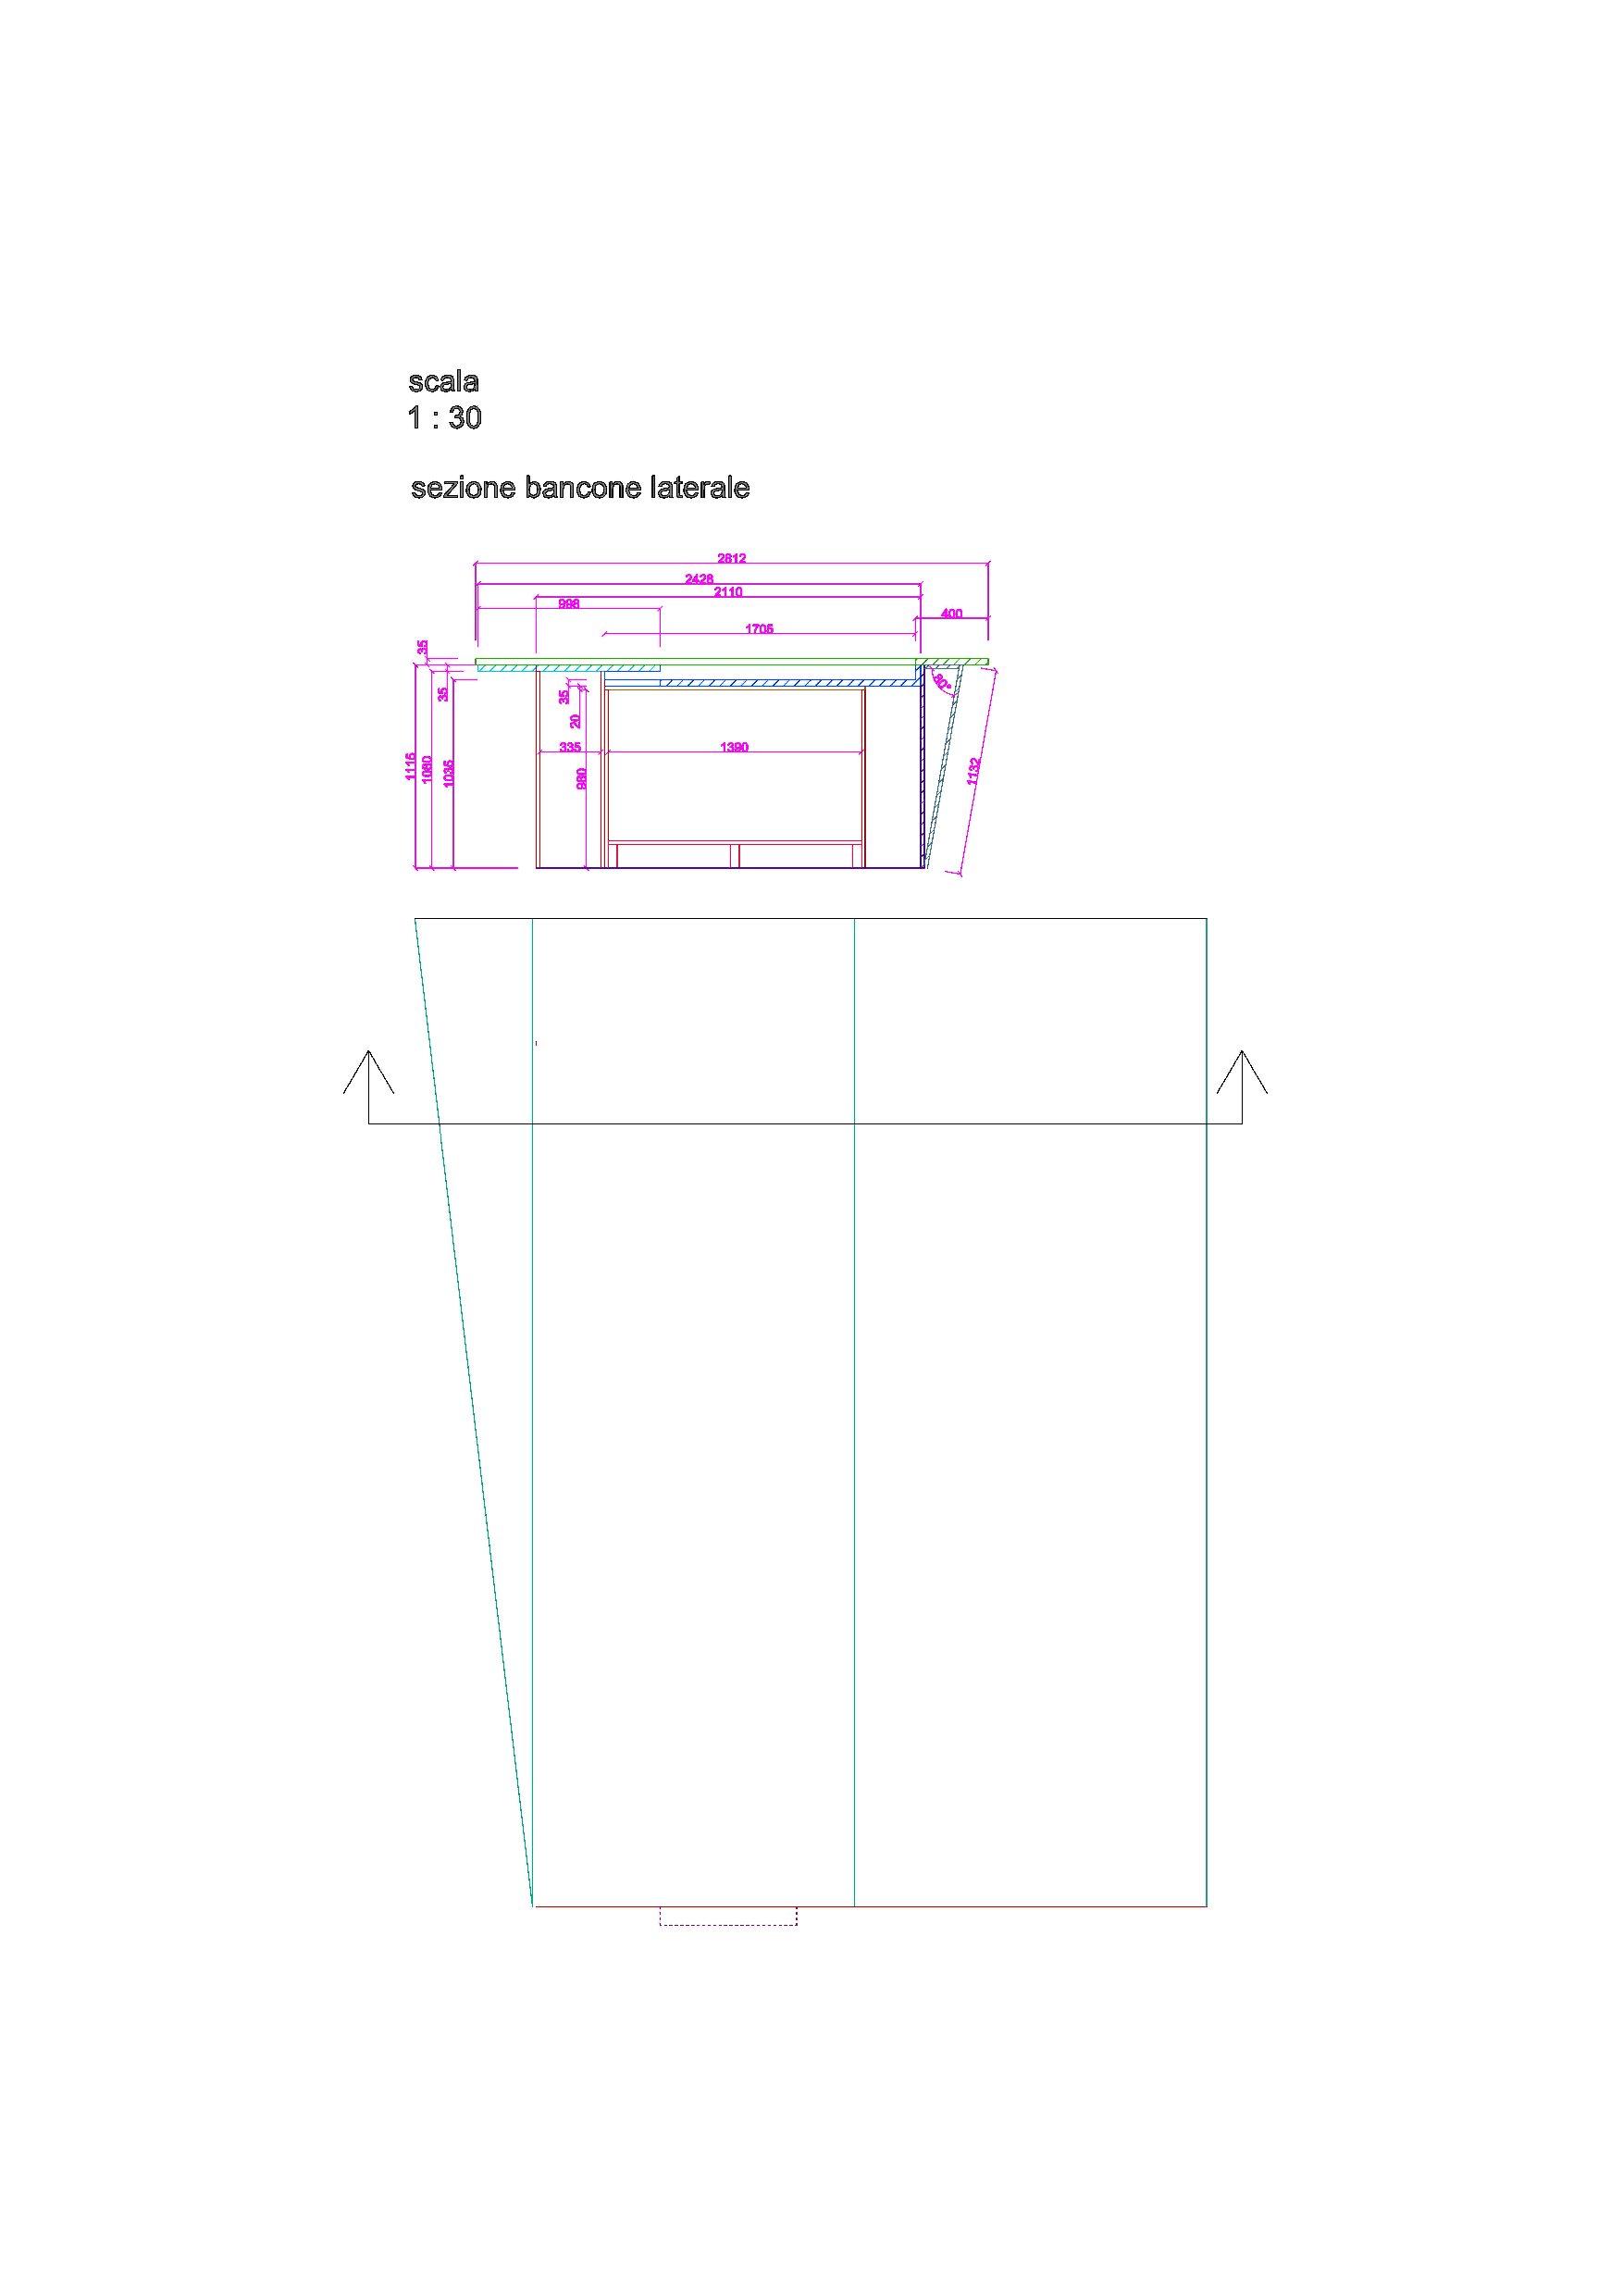
\includegraphics[width=1\linewidth]{25}
\end{figure}

\newpage
\begin{figure}[H]
	\centering
	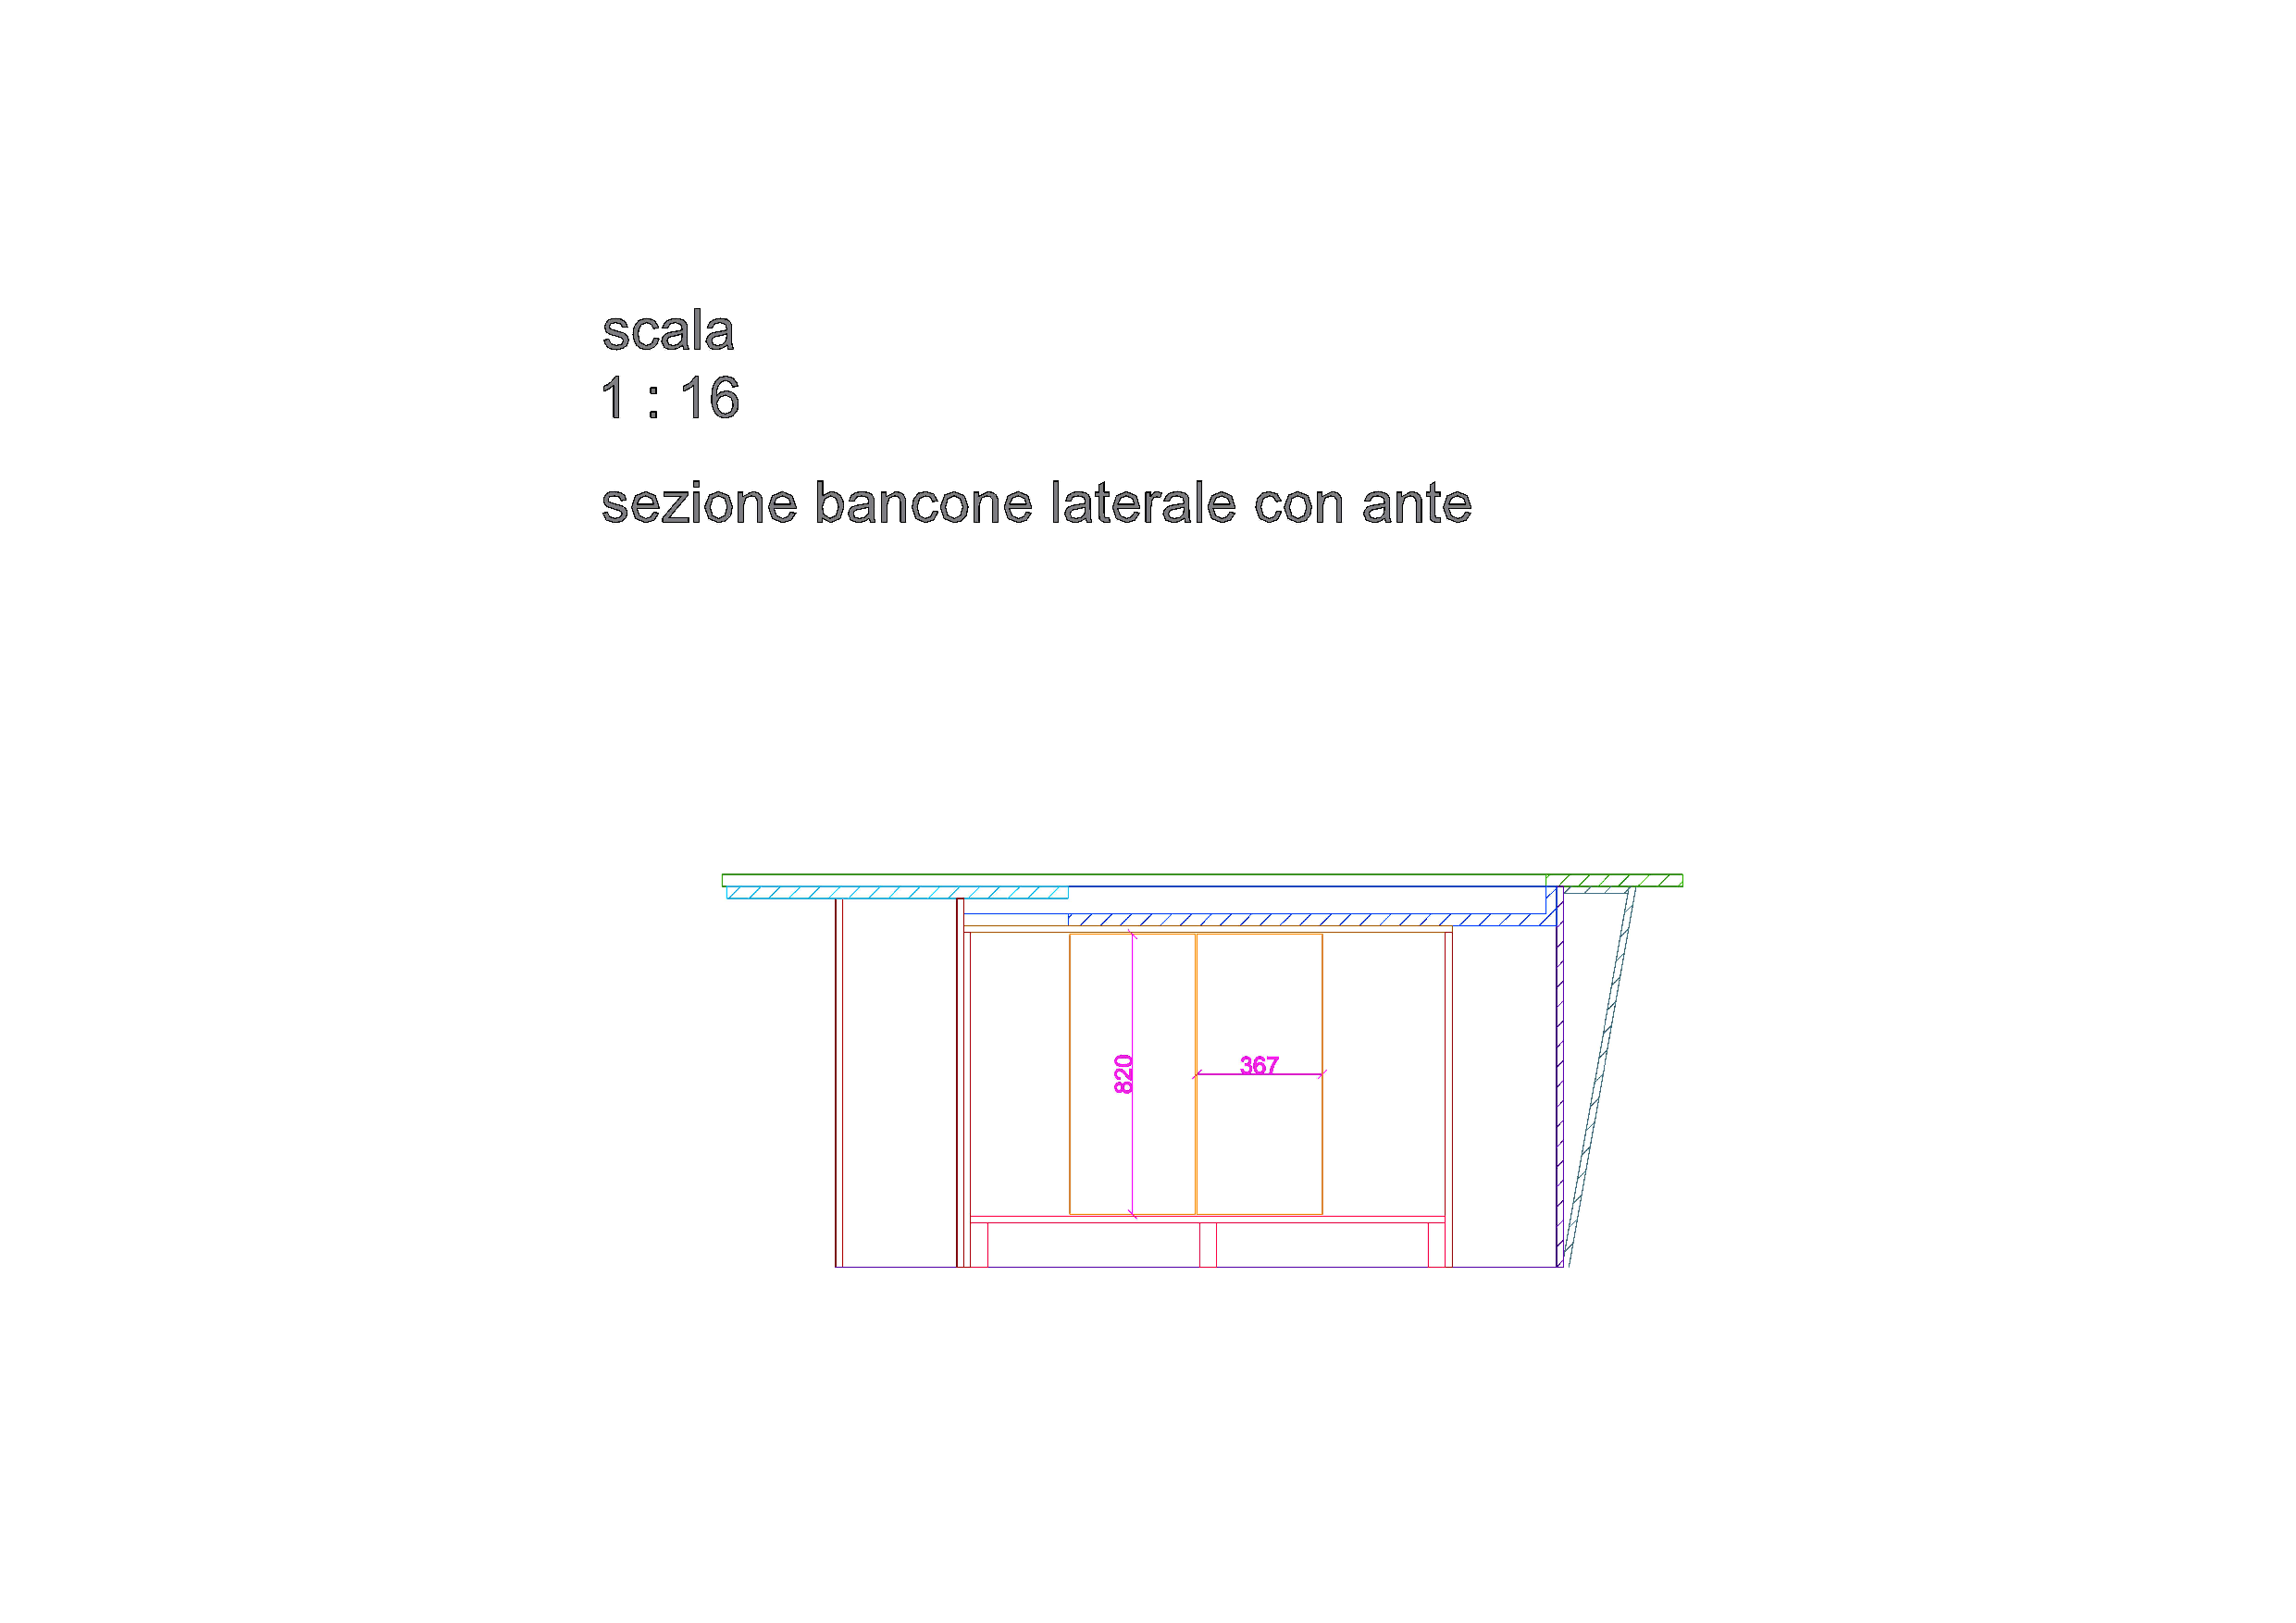
\includegraphics[width=0.8\linewidth]{26}
\end{figure}

\begin{figure}[H]
	\centering
	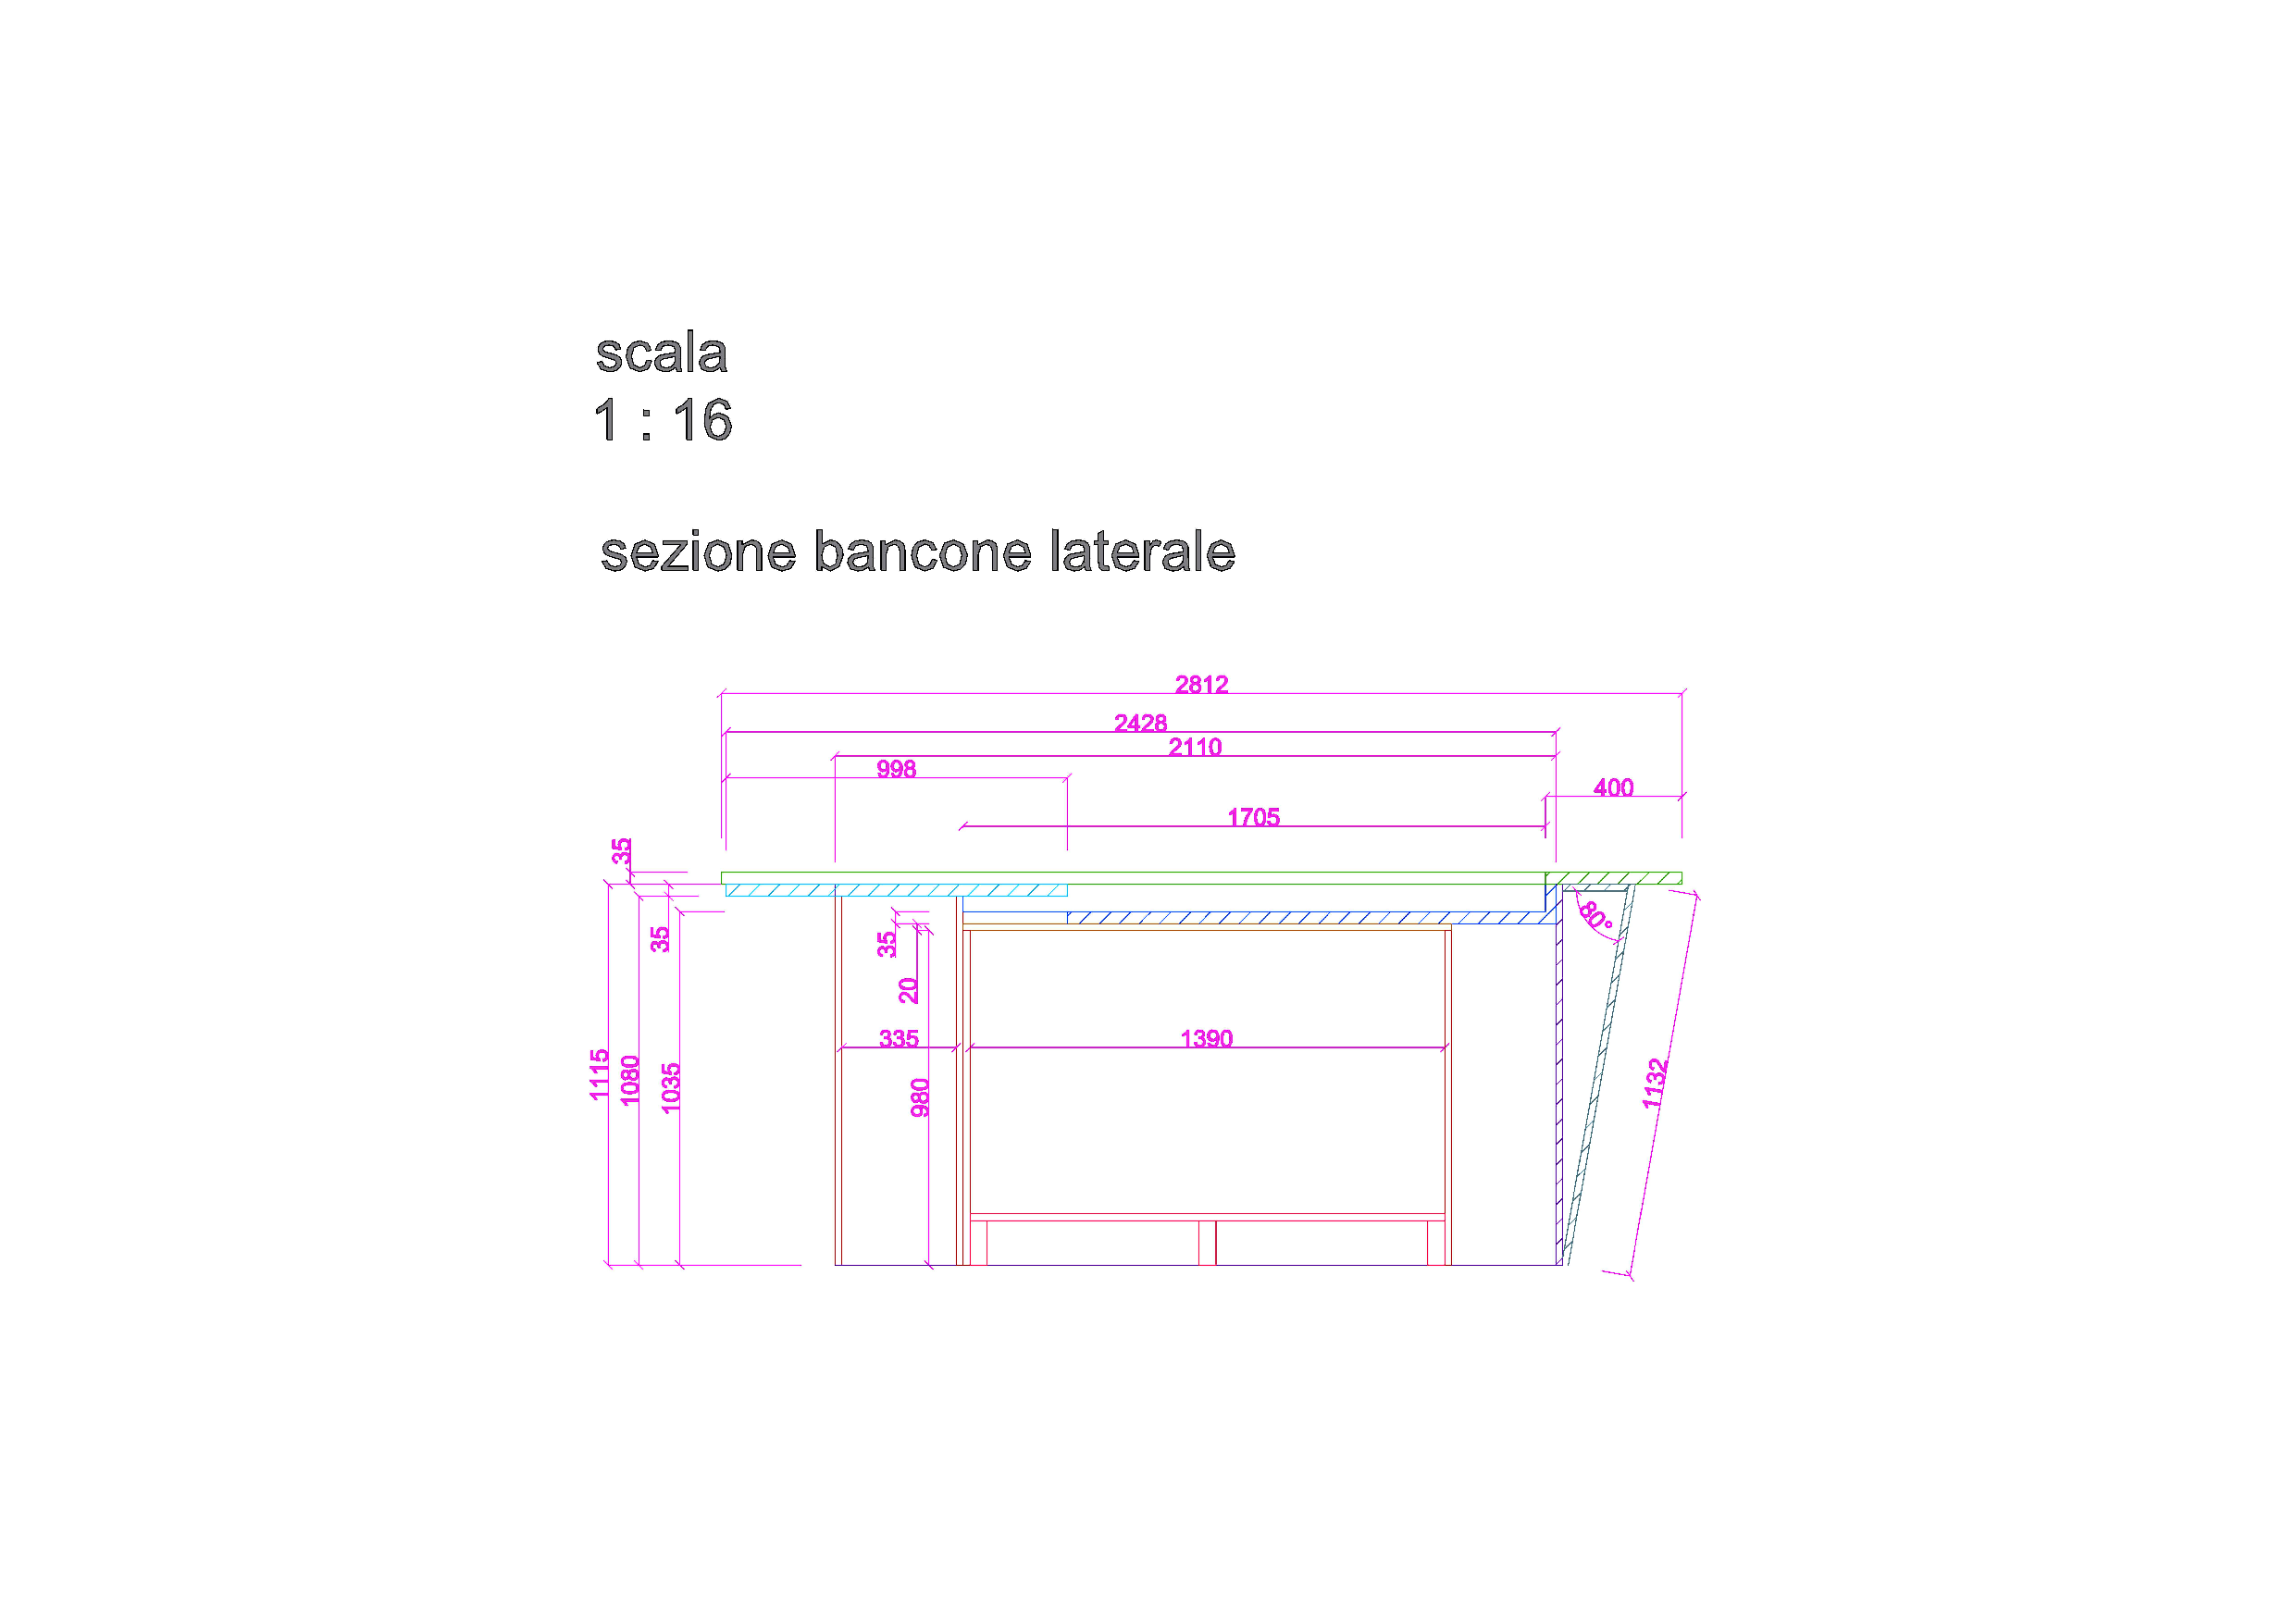
\includegraphics[width=0.8\linewidth]{27}
\end{figure}

\begin{figure}[H]
	\centering
	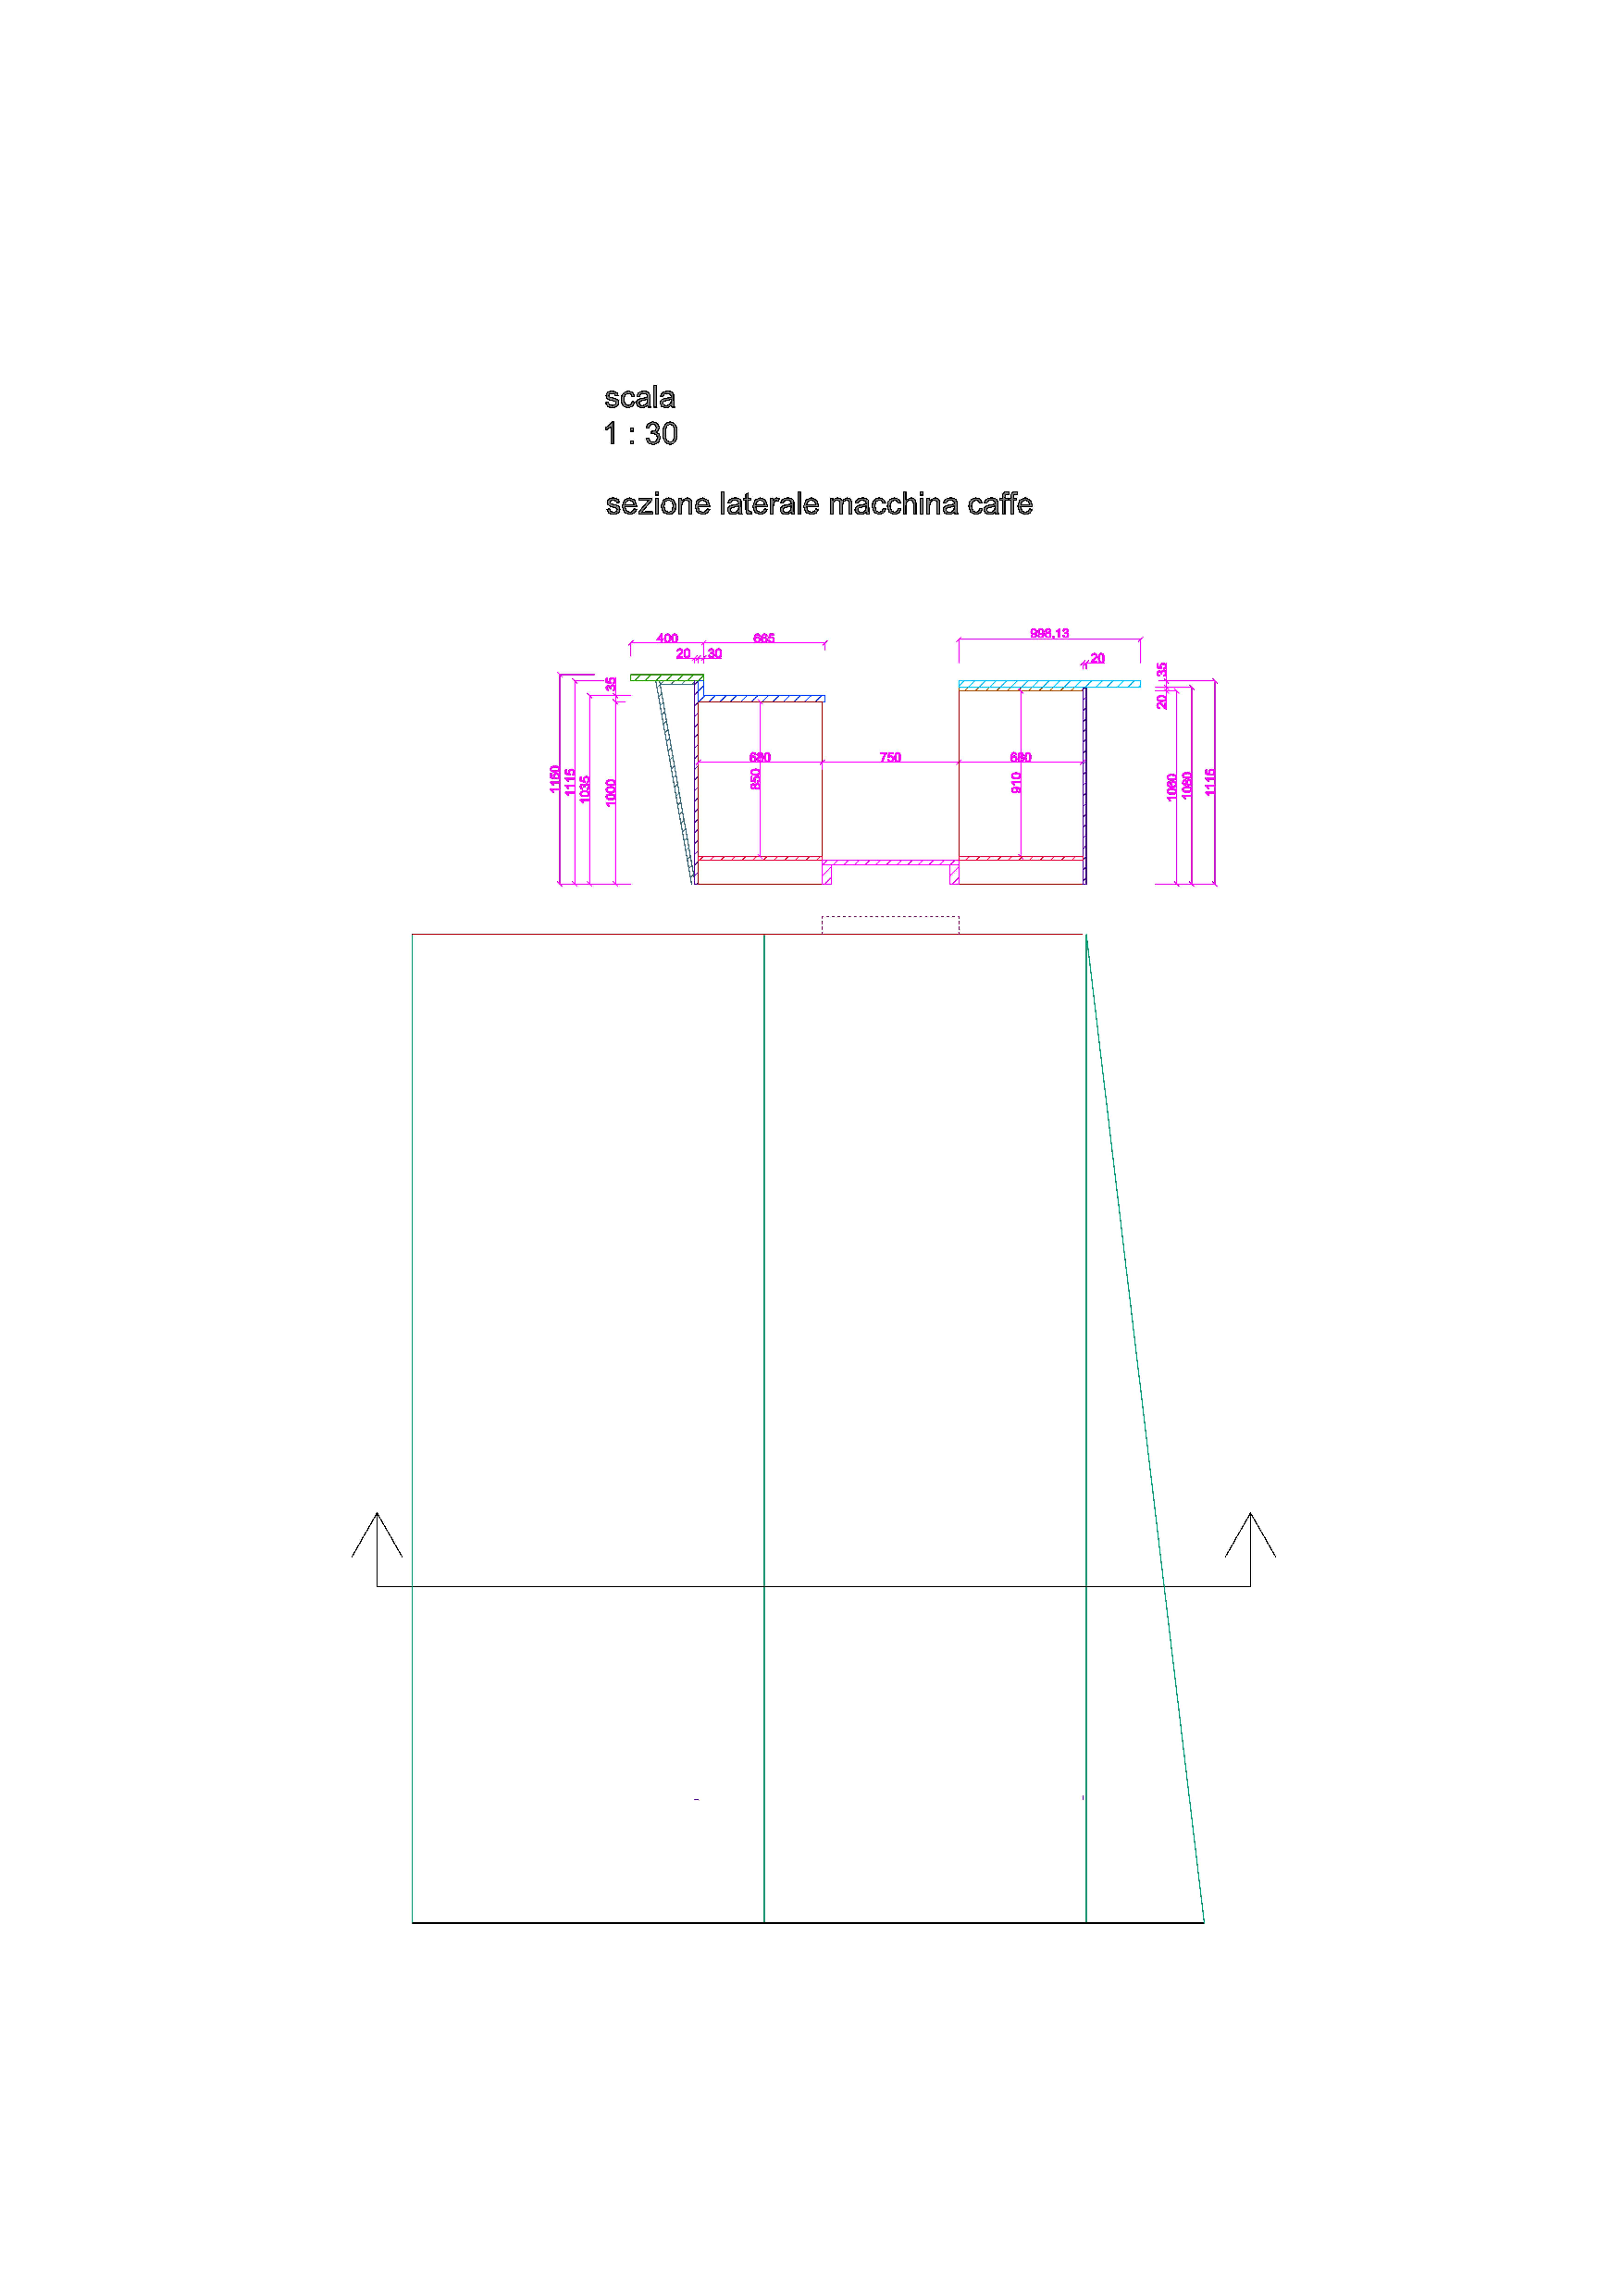
\includegraphics[width=1\linewidth]{28}
\end{figure}

\newpage
\begin{figure}[H]
	\centering
	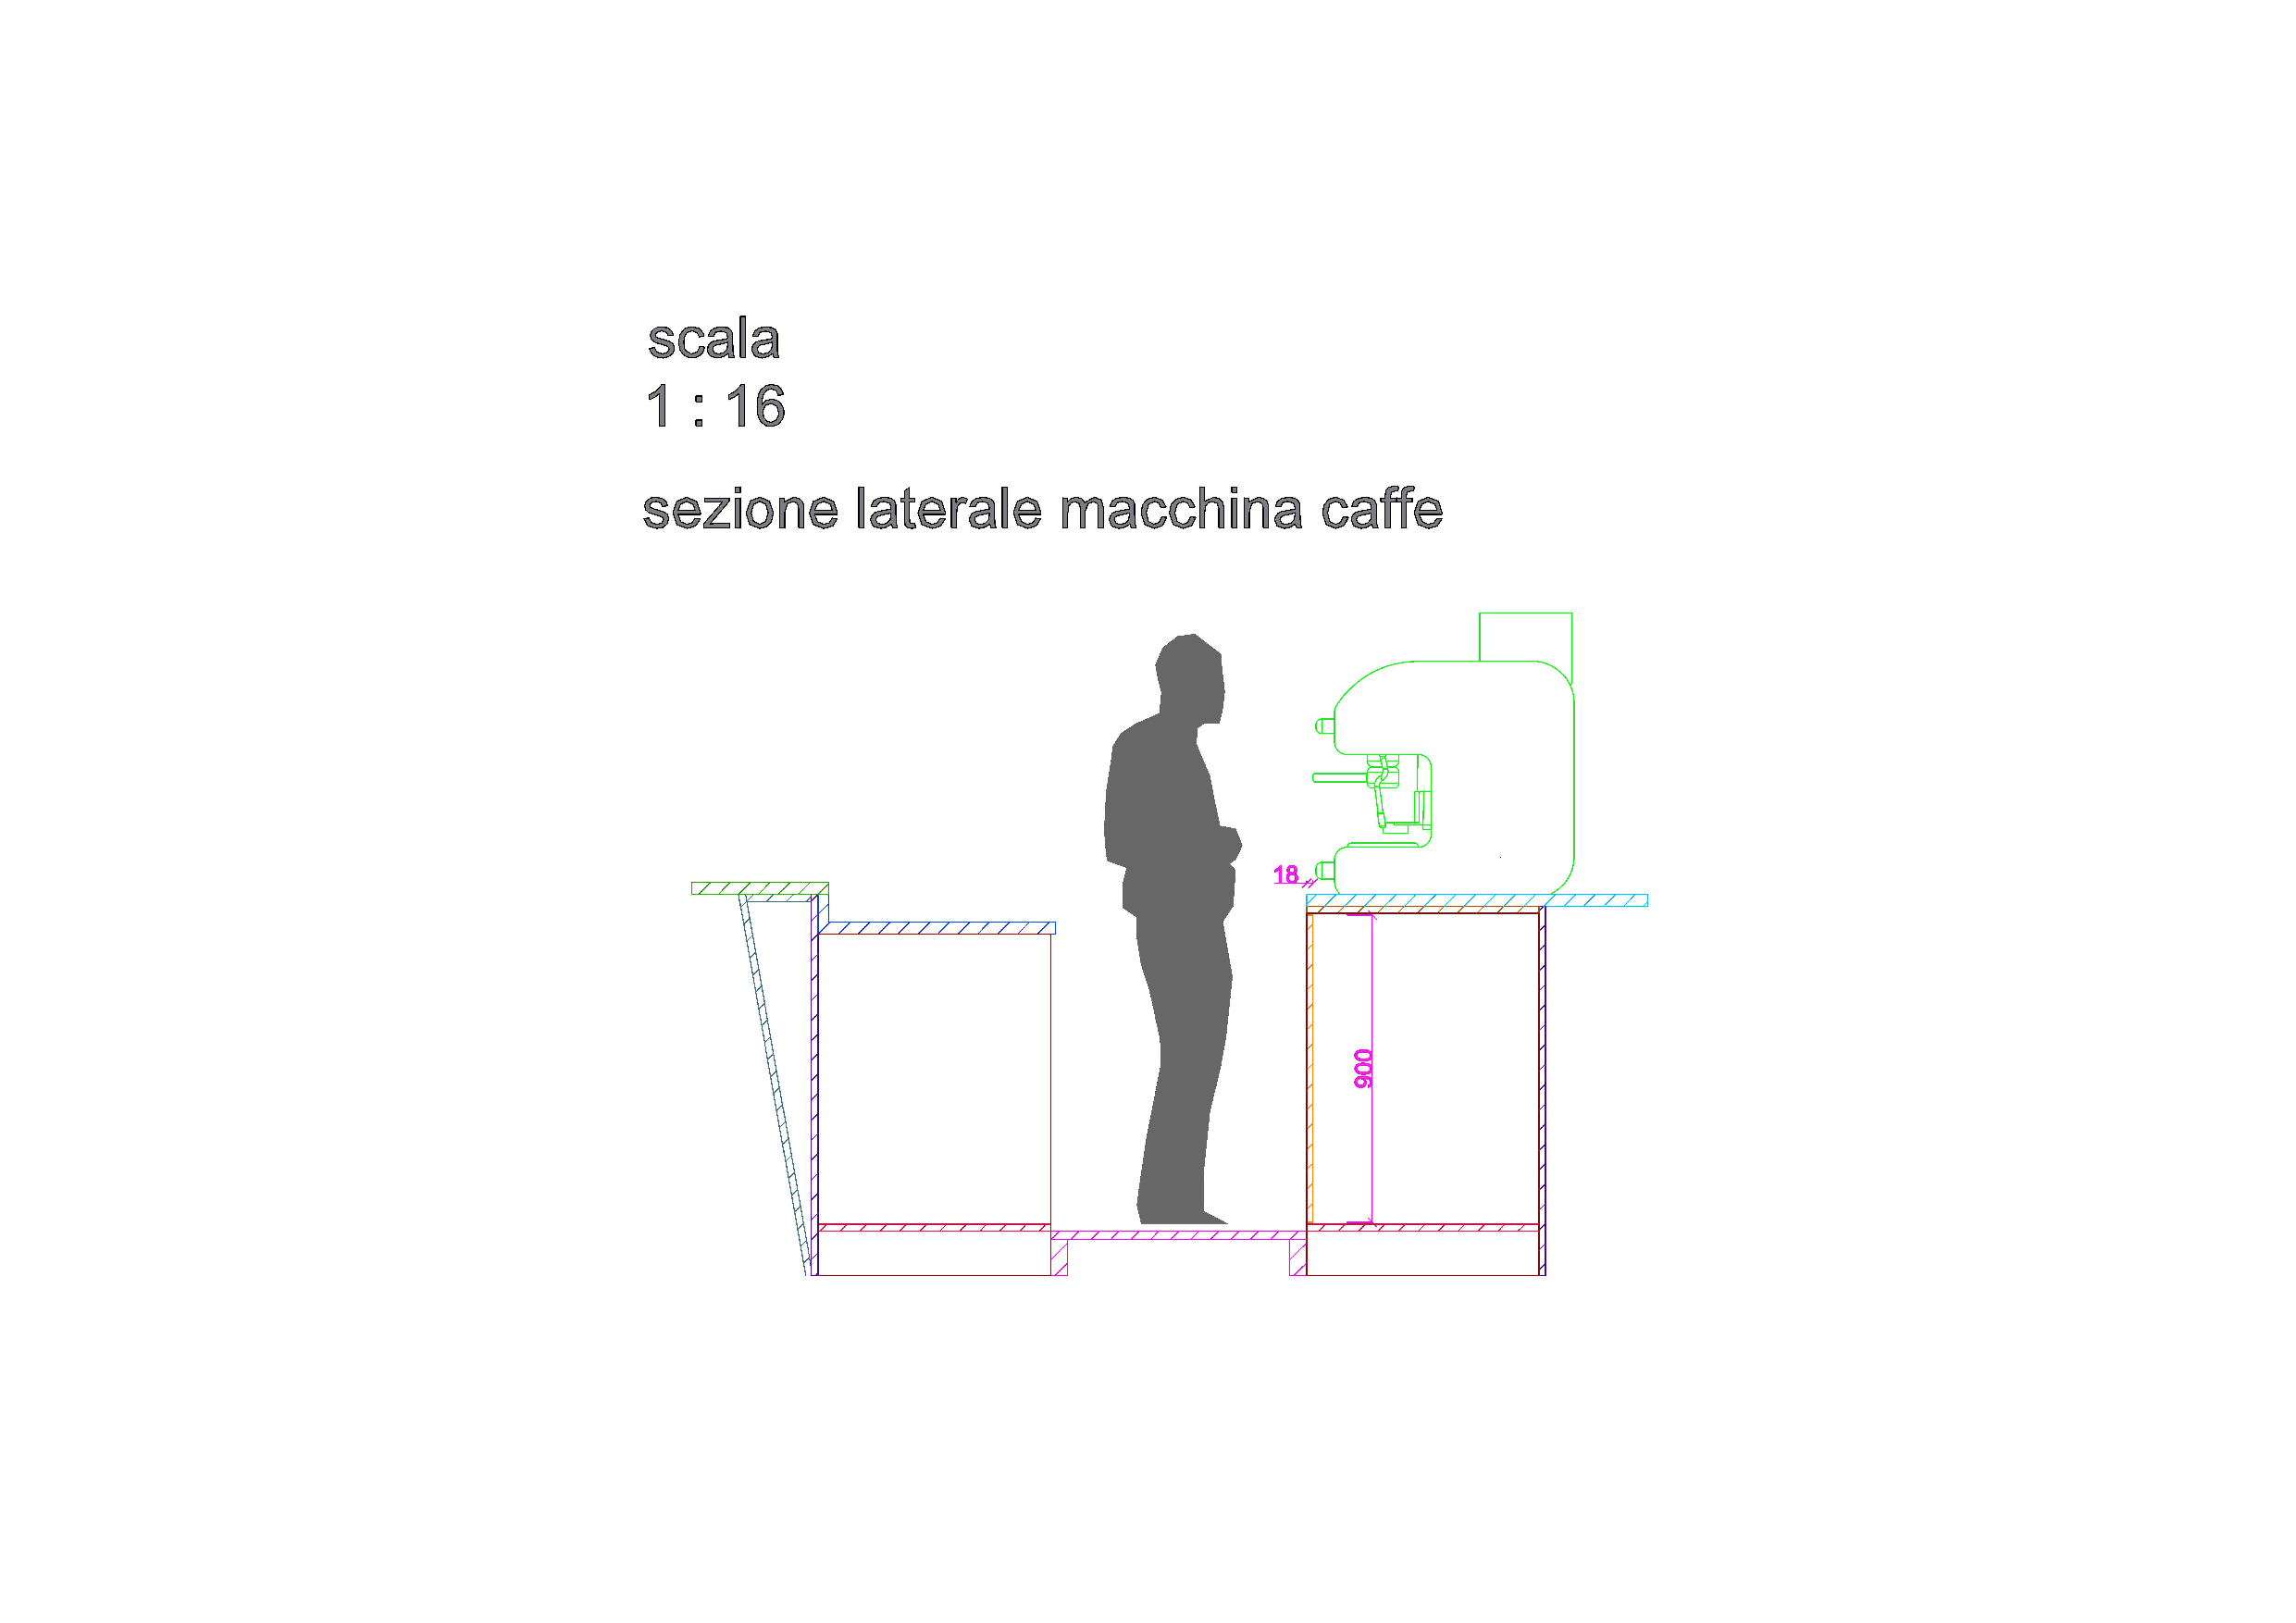
\includegraphics[width=0.8\linewidth]{29}
\end{figure}

\begin{figure}[H]
	\centering
	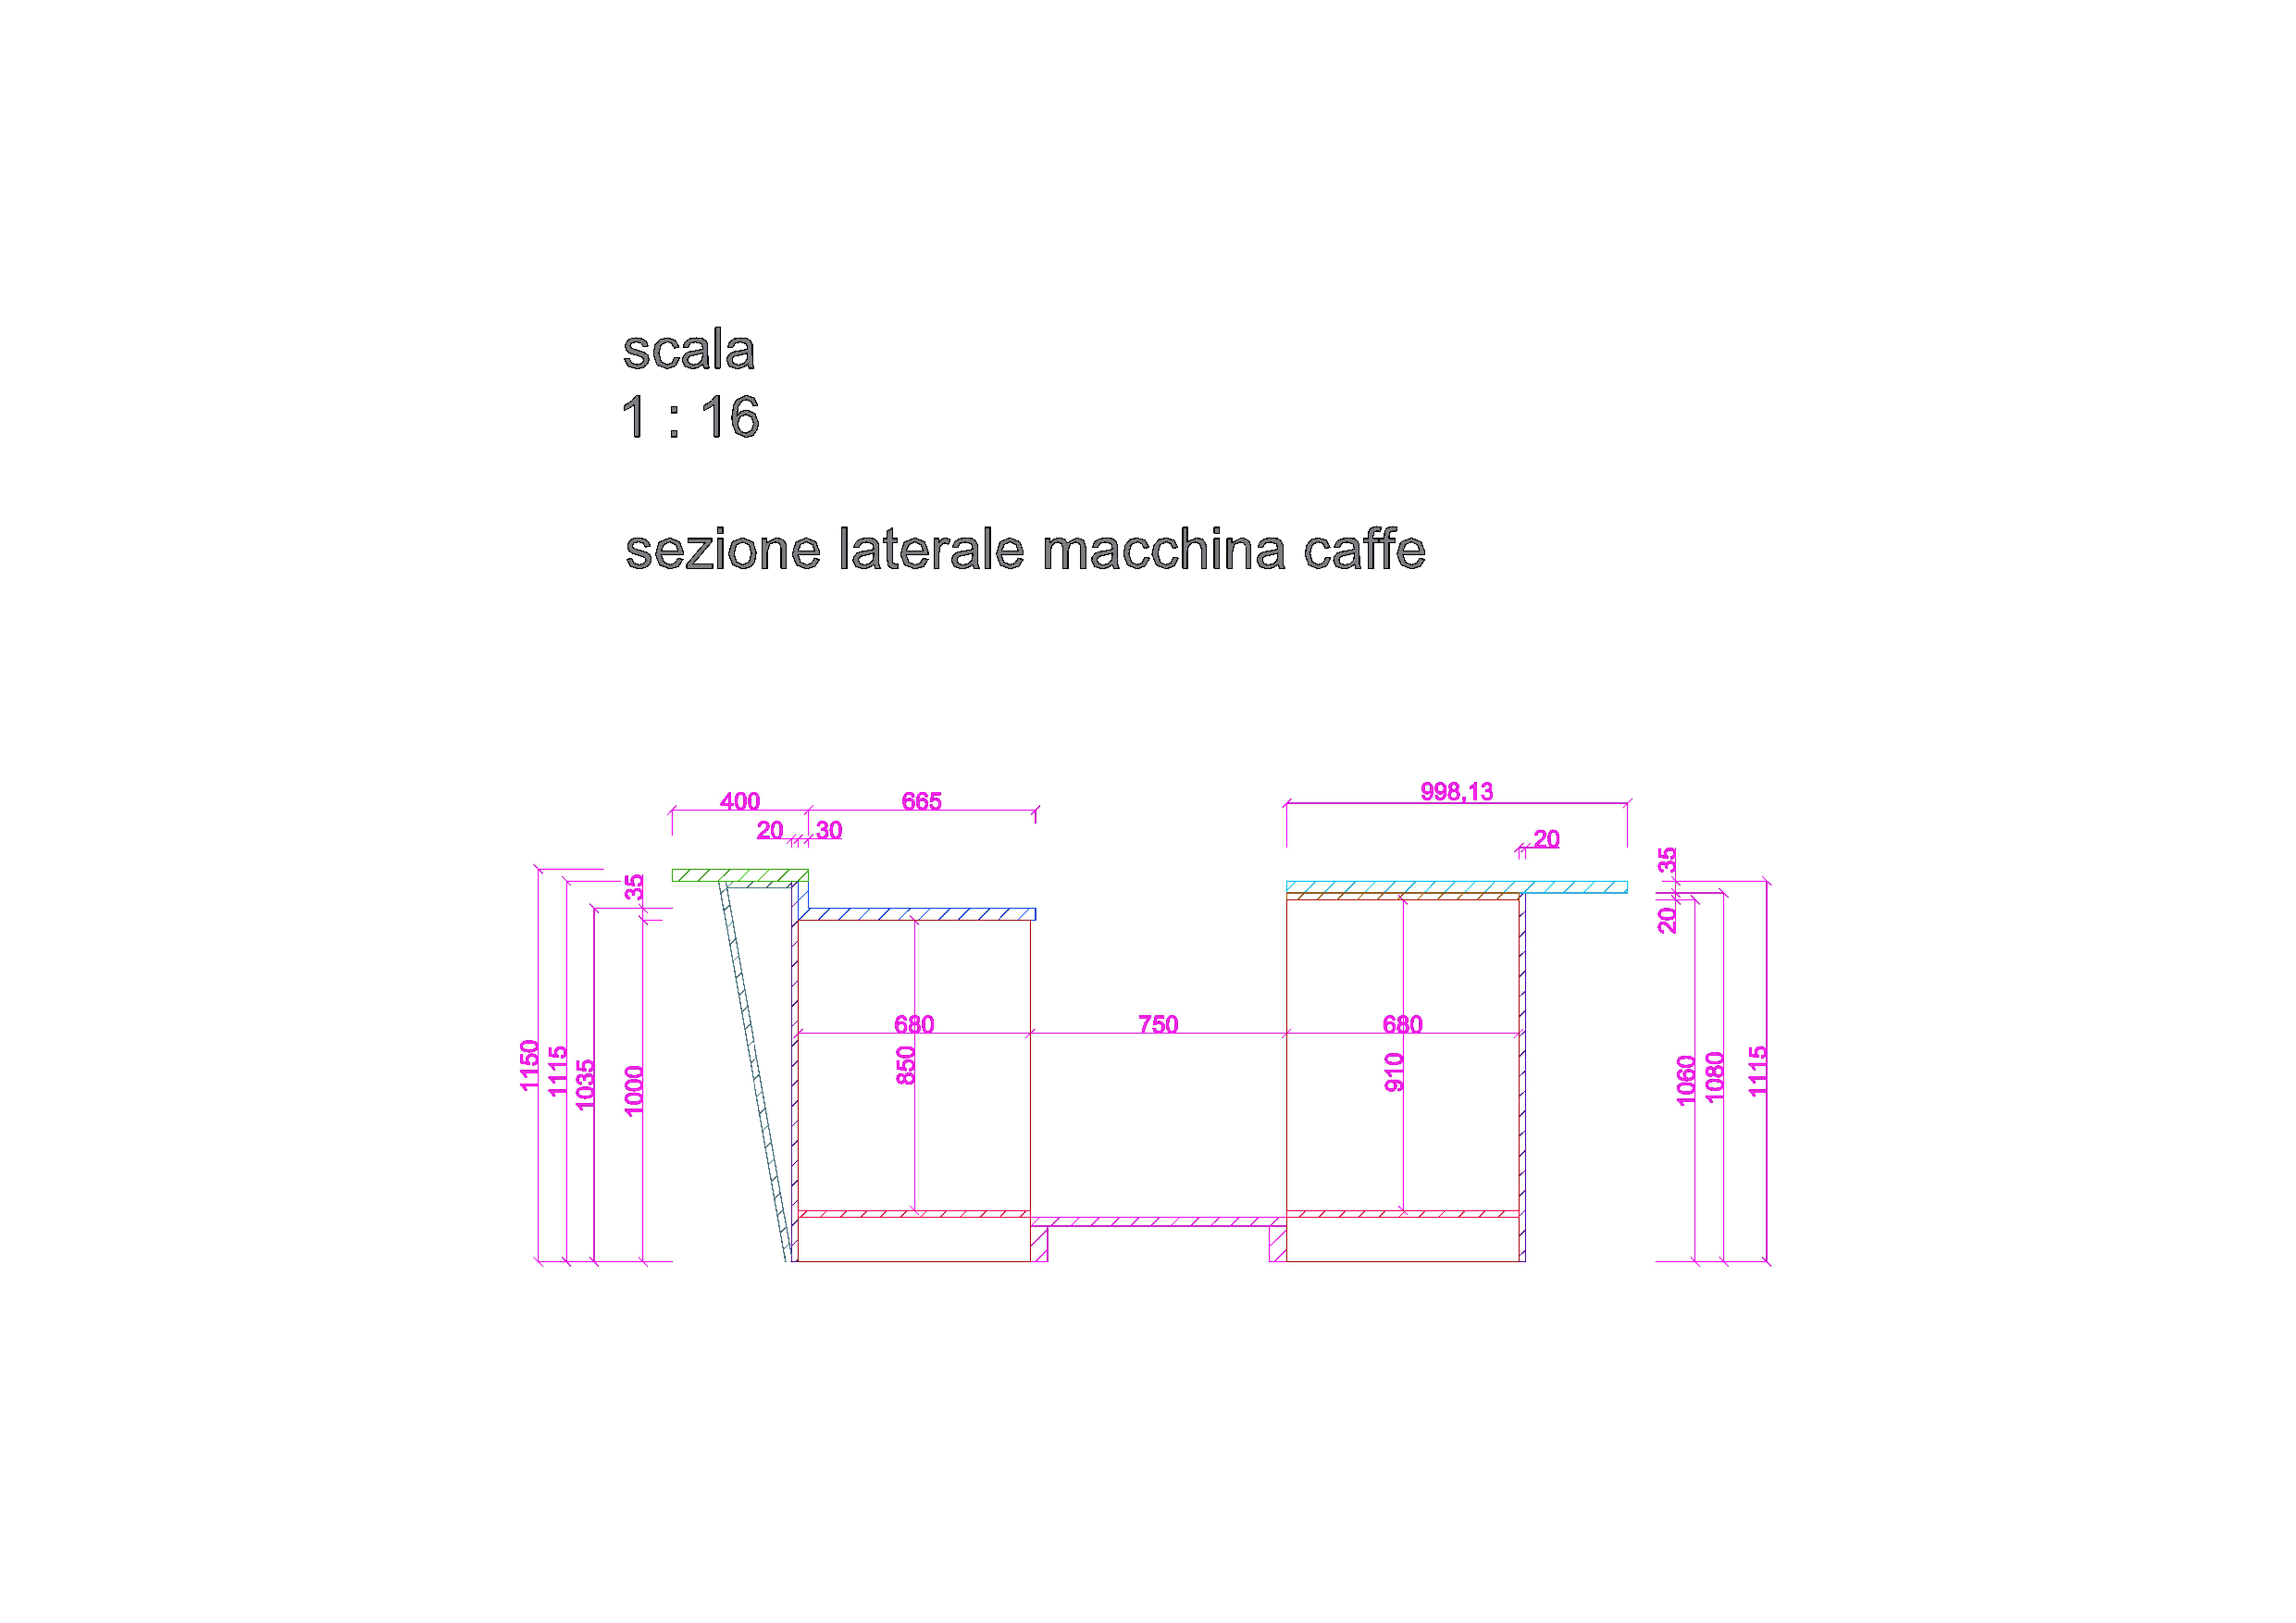
\includegraphics[width=0.8\linewidth]{30}
\end{figure}

% --------------------------------

\begin{figure}[H]
	\centering
	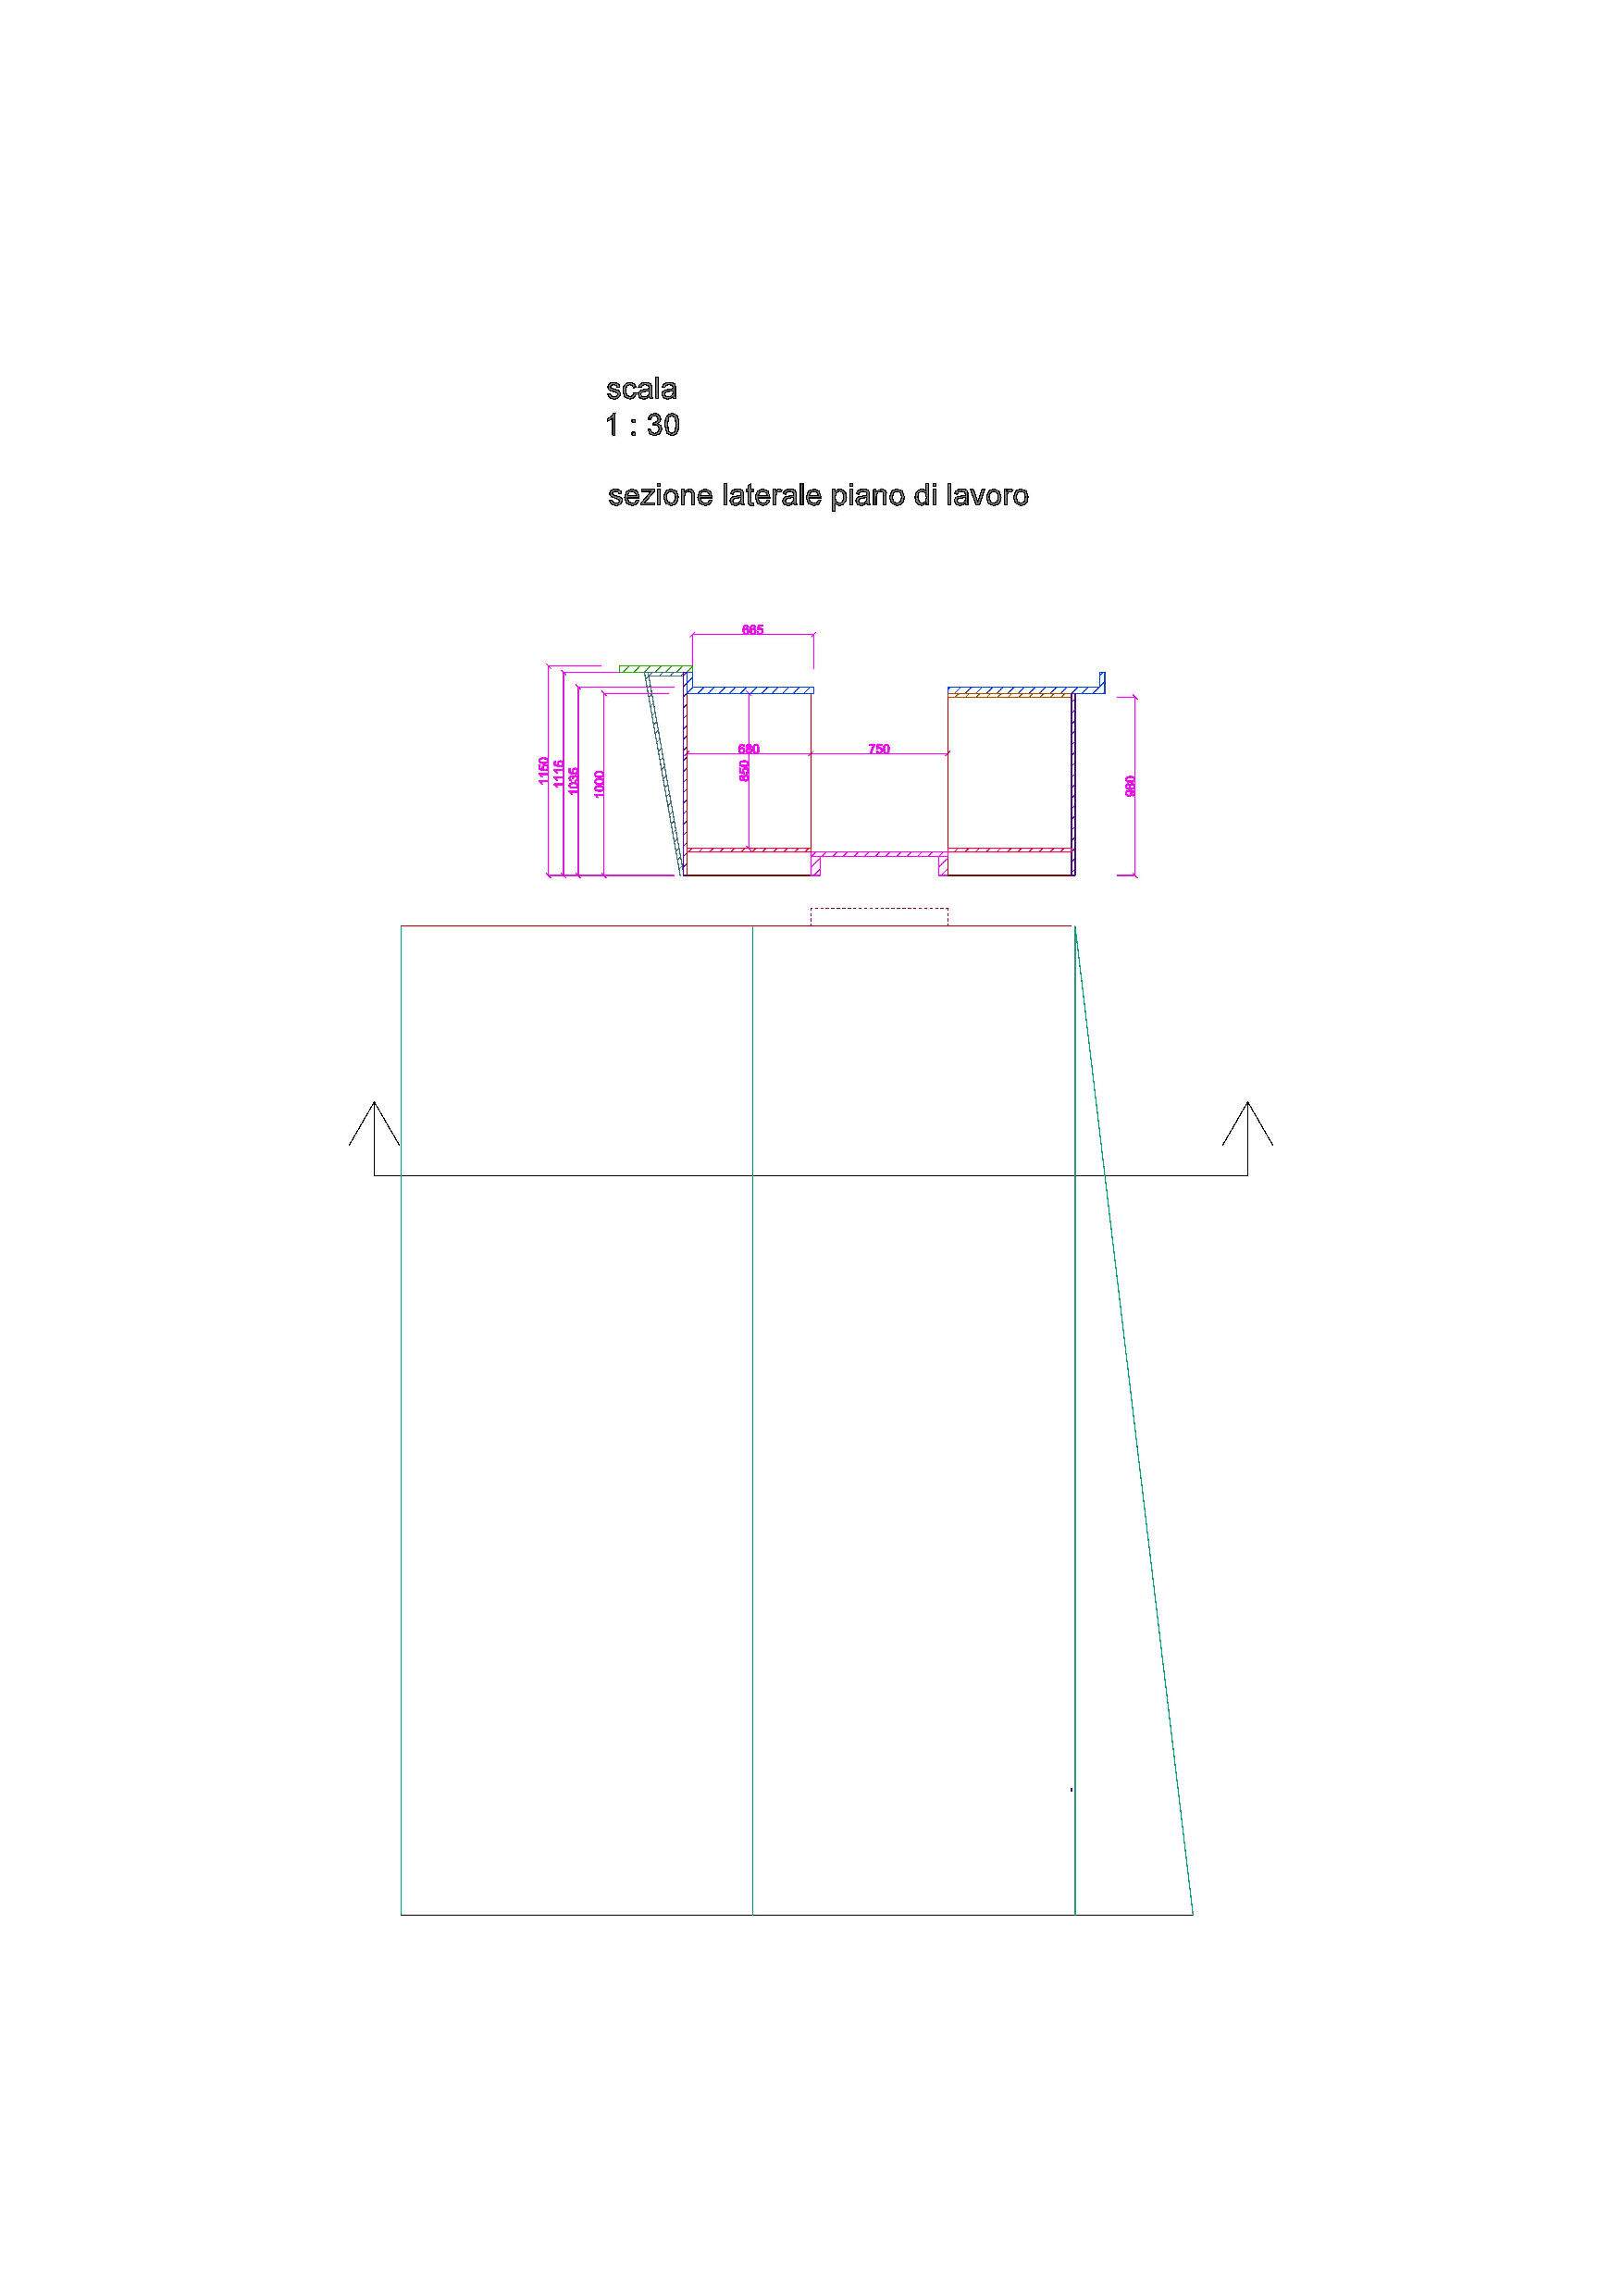
\includegraphics[width=1\linewidth]{31}
\end{figure}


\newpage
\begin{figure}[H]
	\centering
	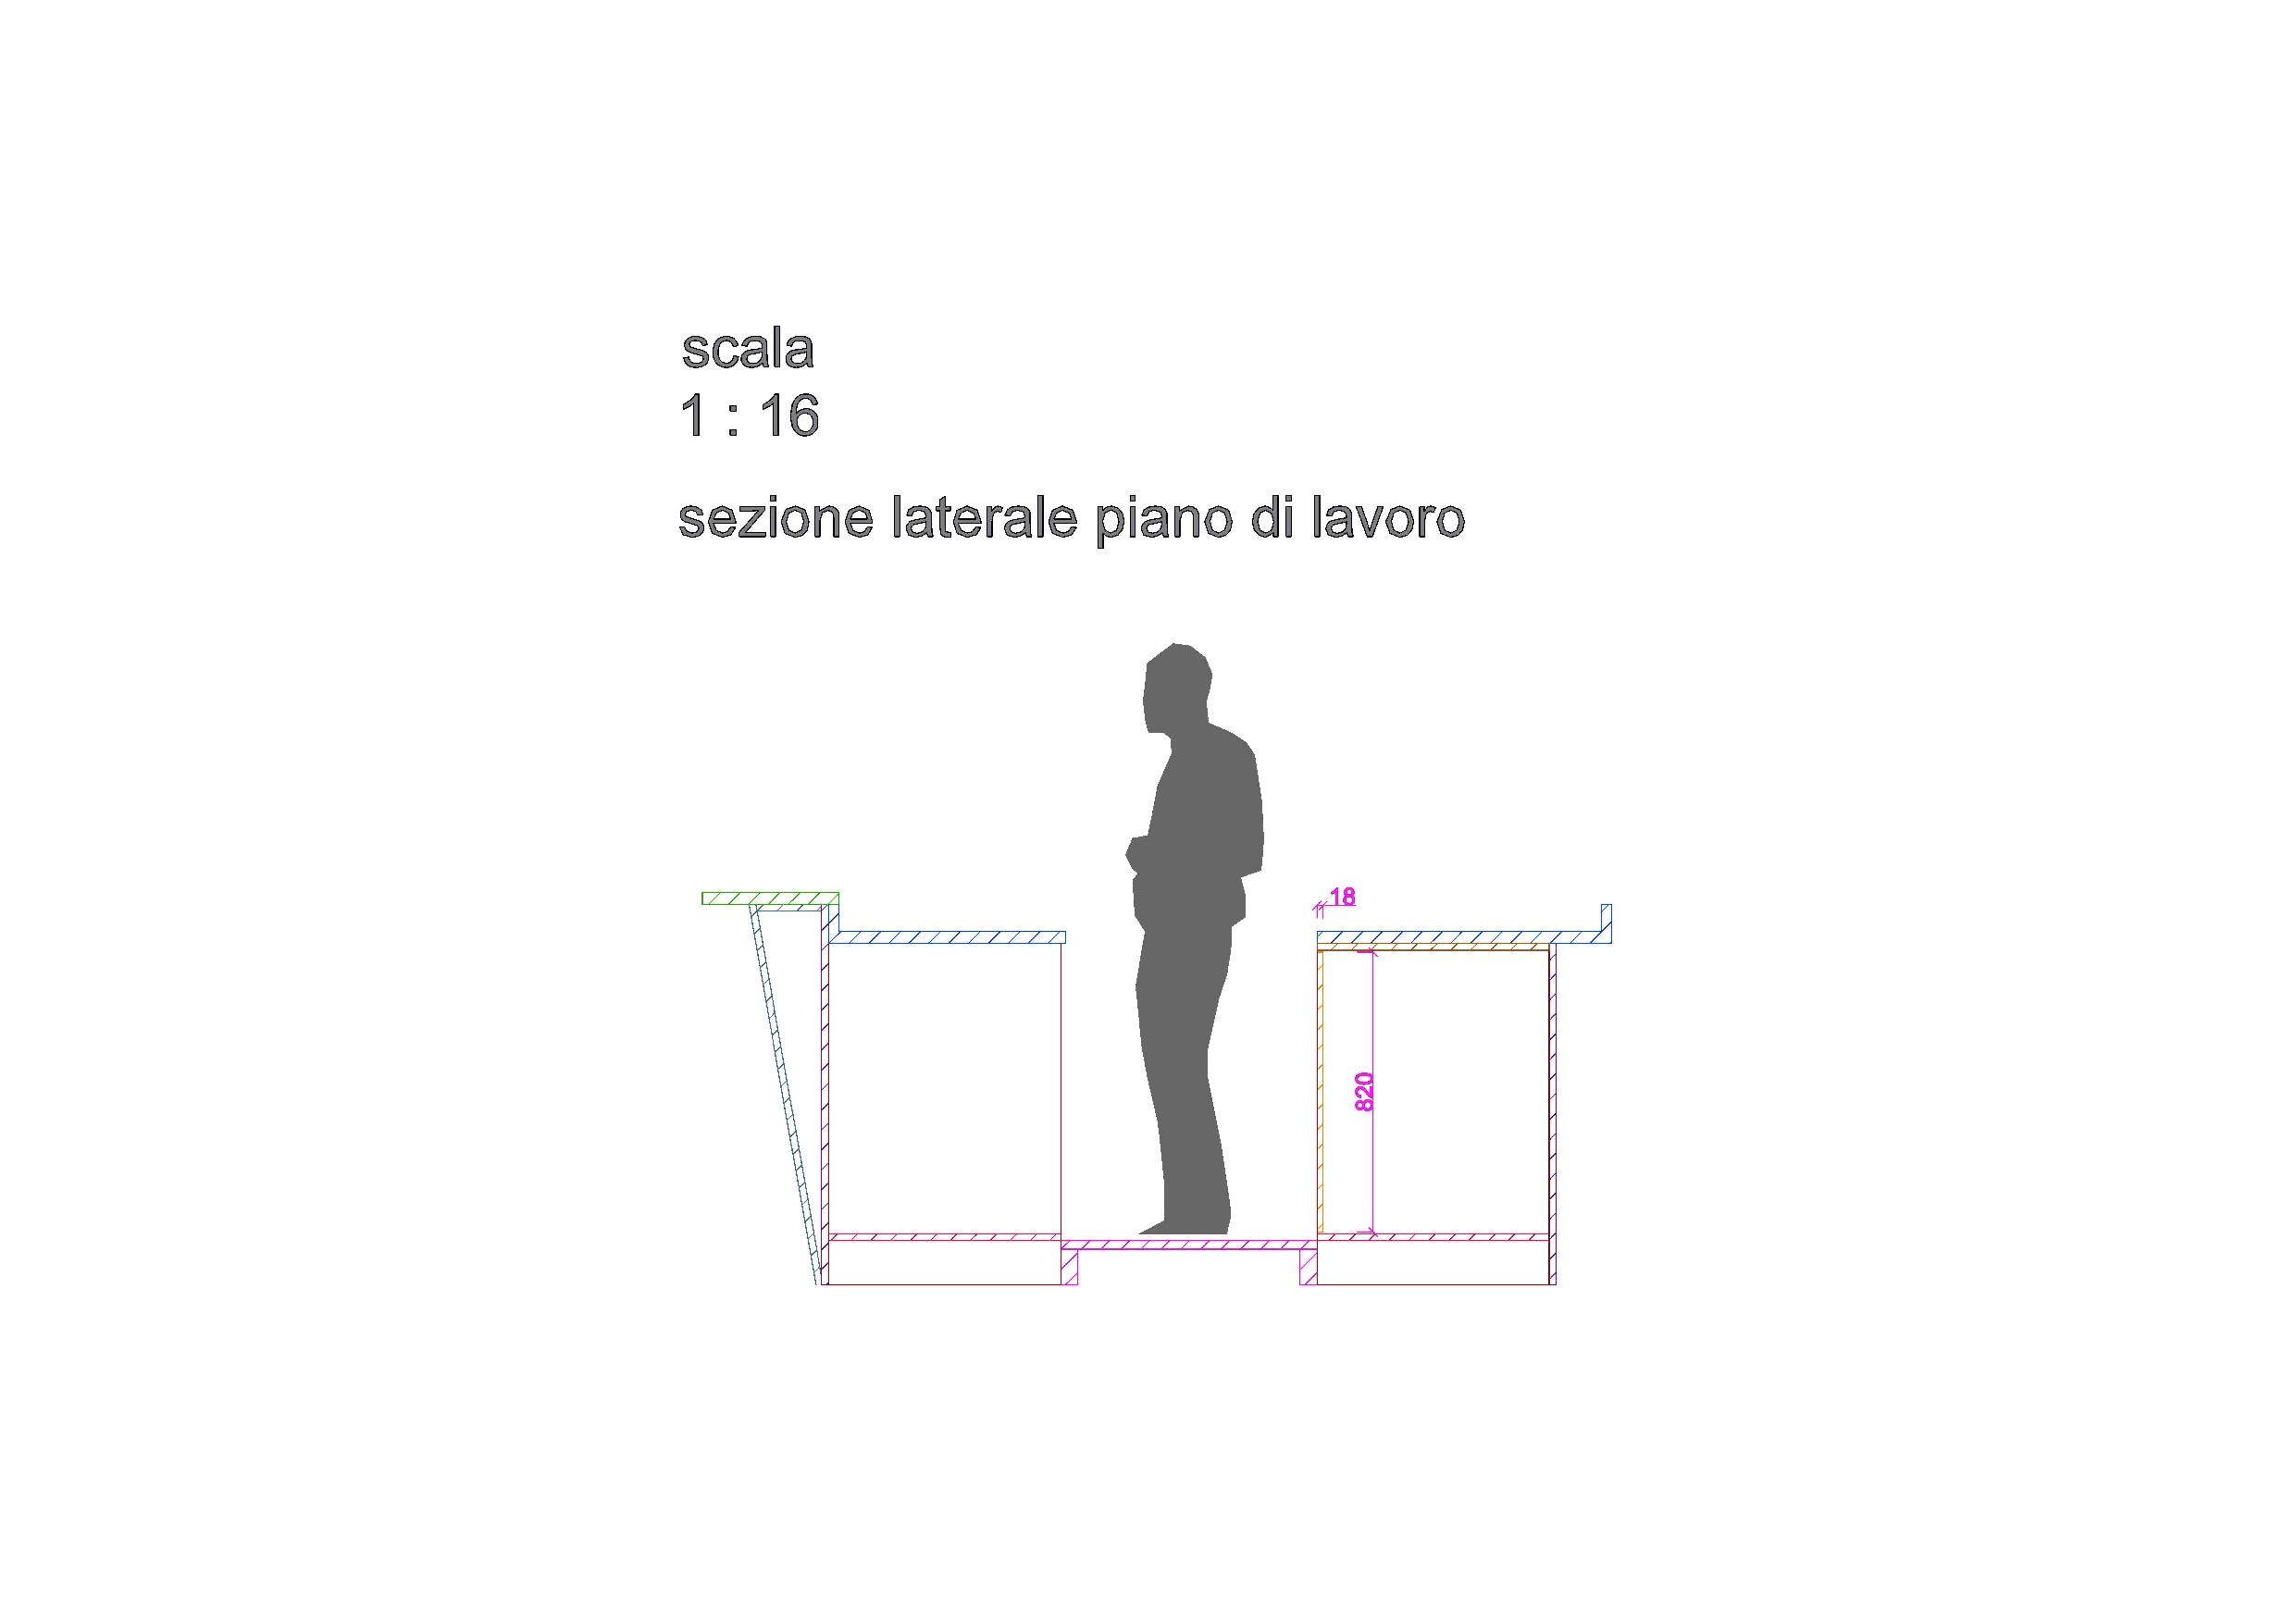
\includegraphics[width=0.8\linewidth]{32}
\end{figure}

\begin{figure}[H]
	\centering
	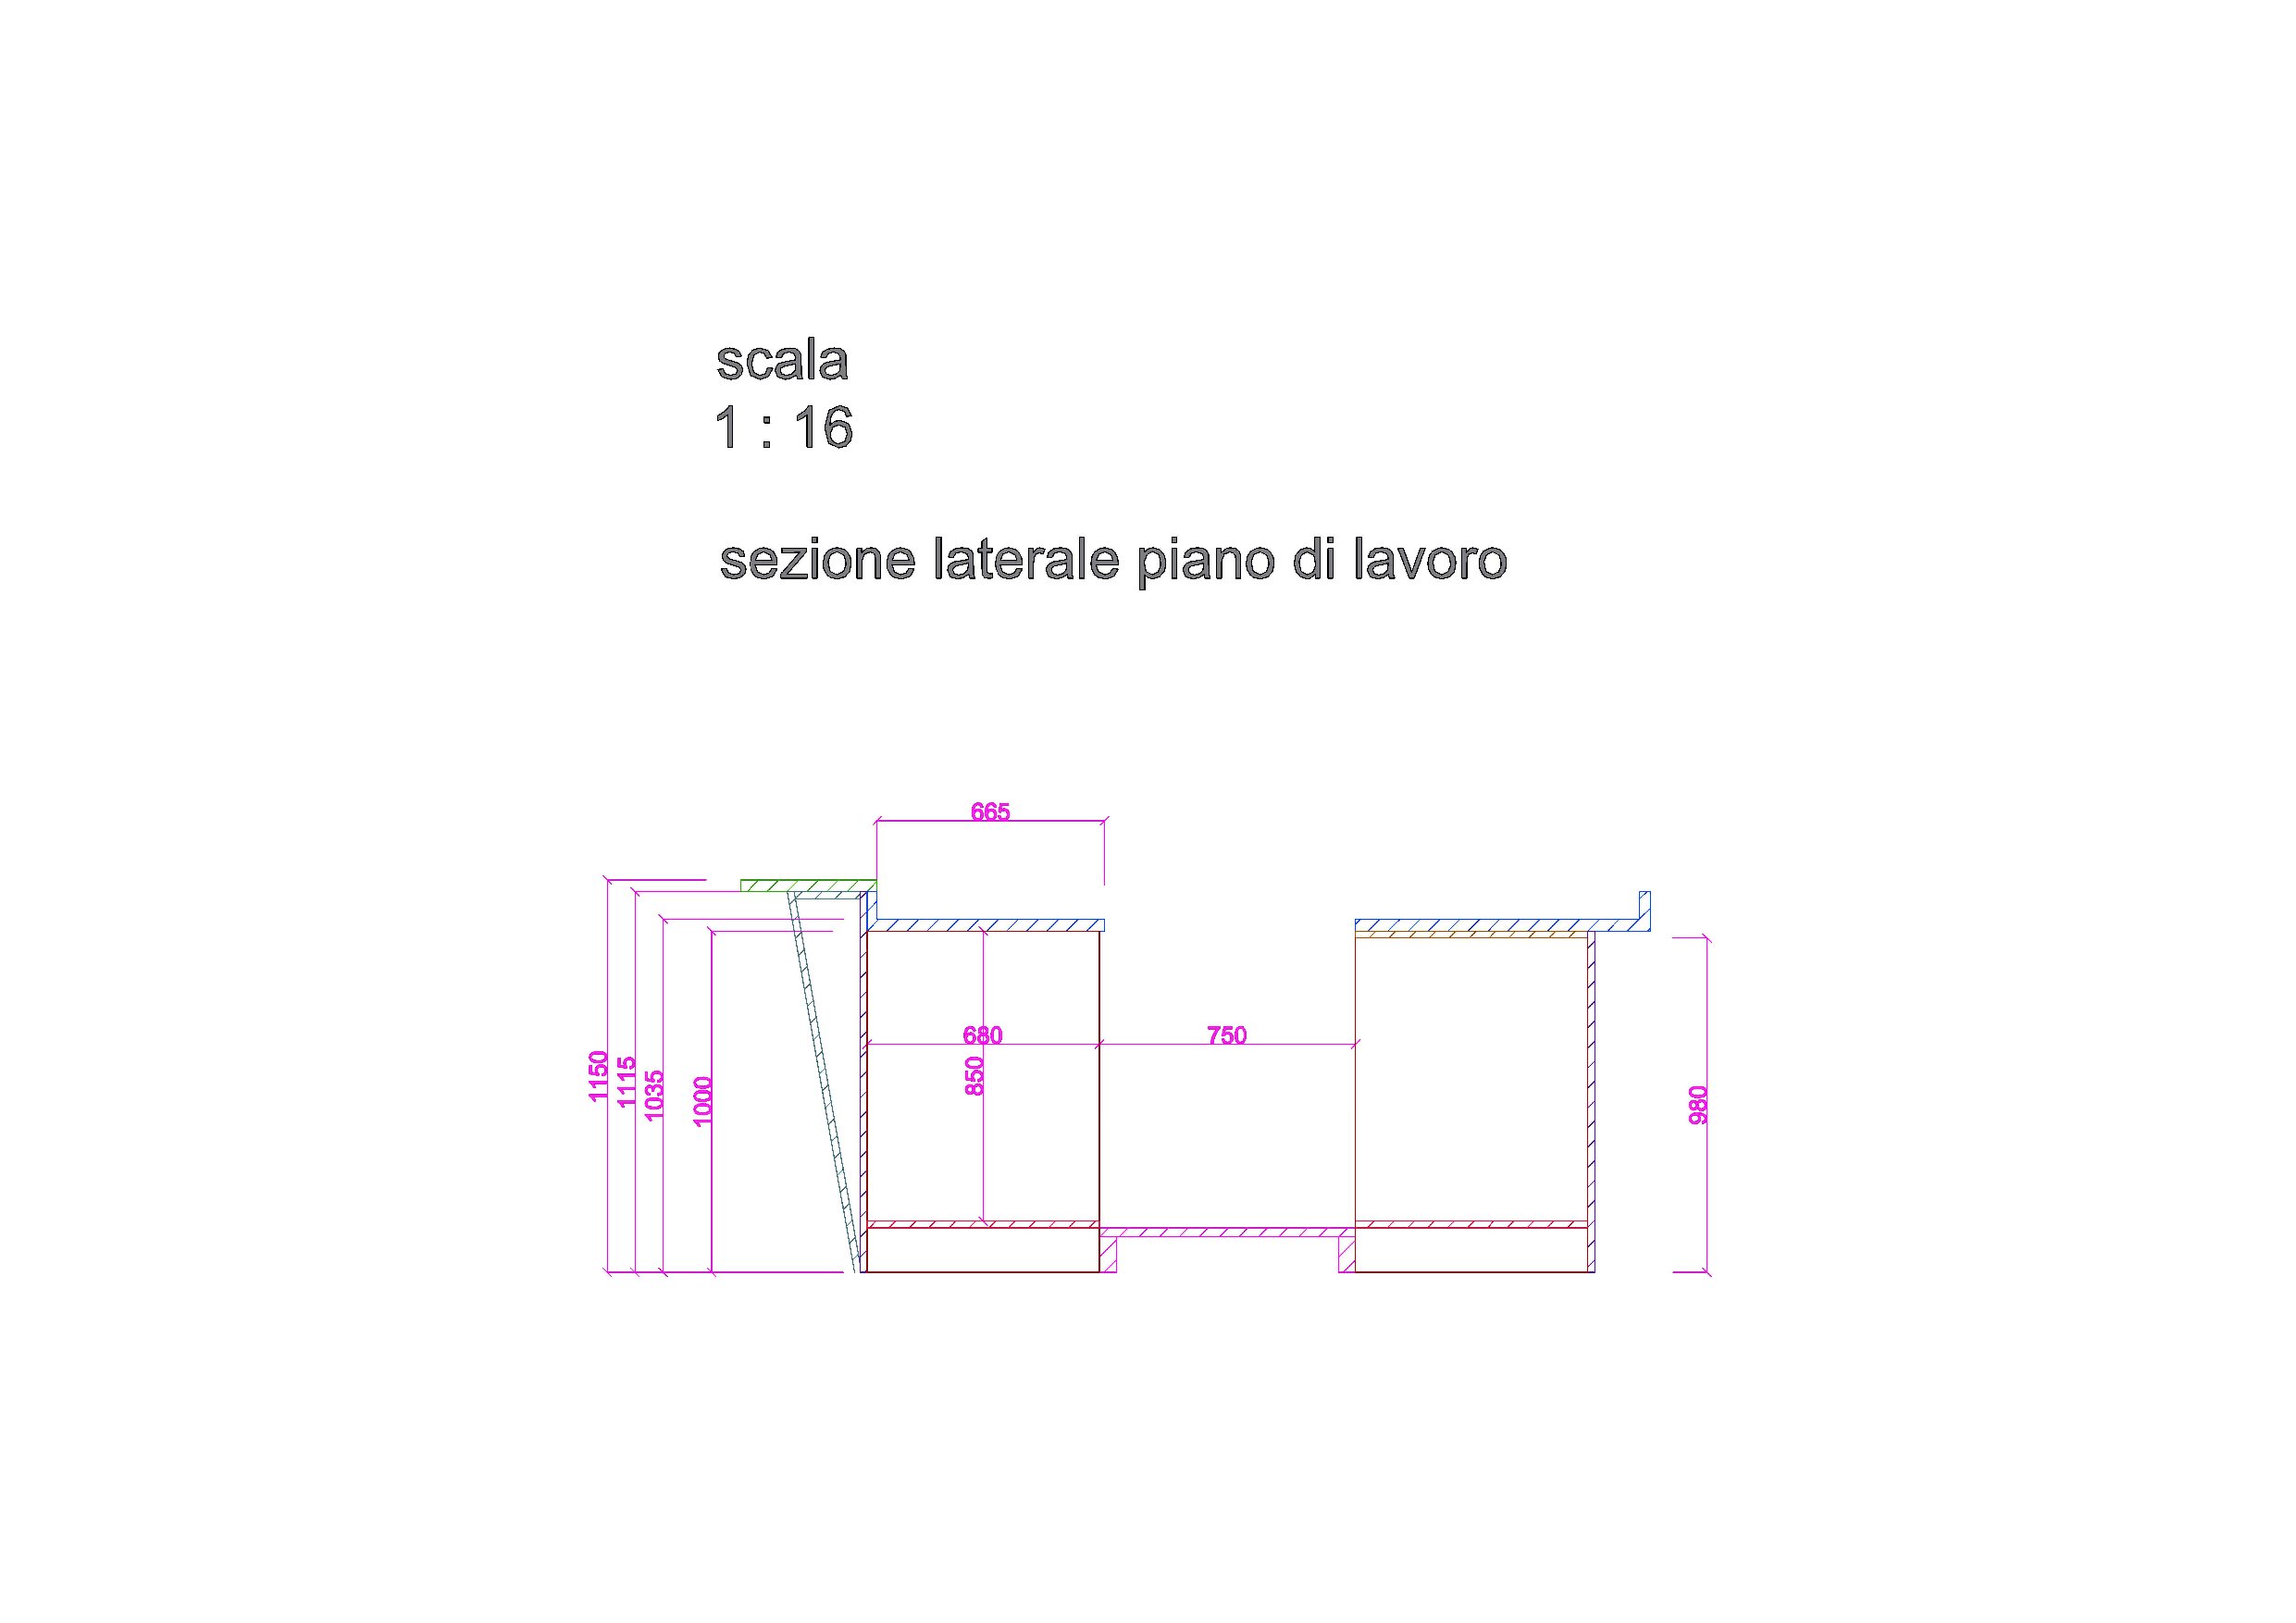
\includegraphics[width=0.8\linewidth]{33}
\end{figure}

\begin{figure}[H]
	\centering
	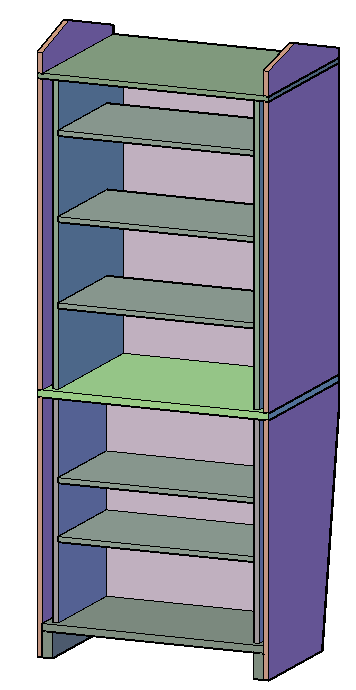
\includegraphics[width=0.7\linewidth]{34}
\end{figure}

\begin{figure}[H]
	\centering
	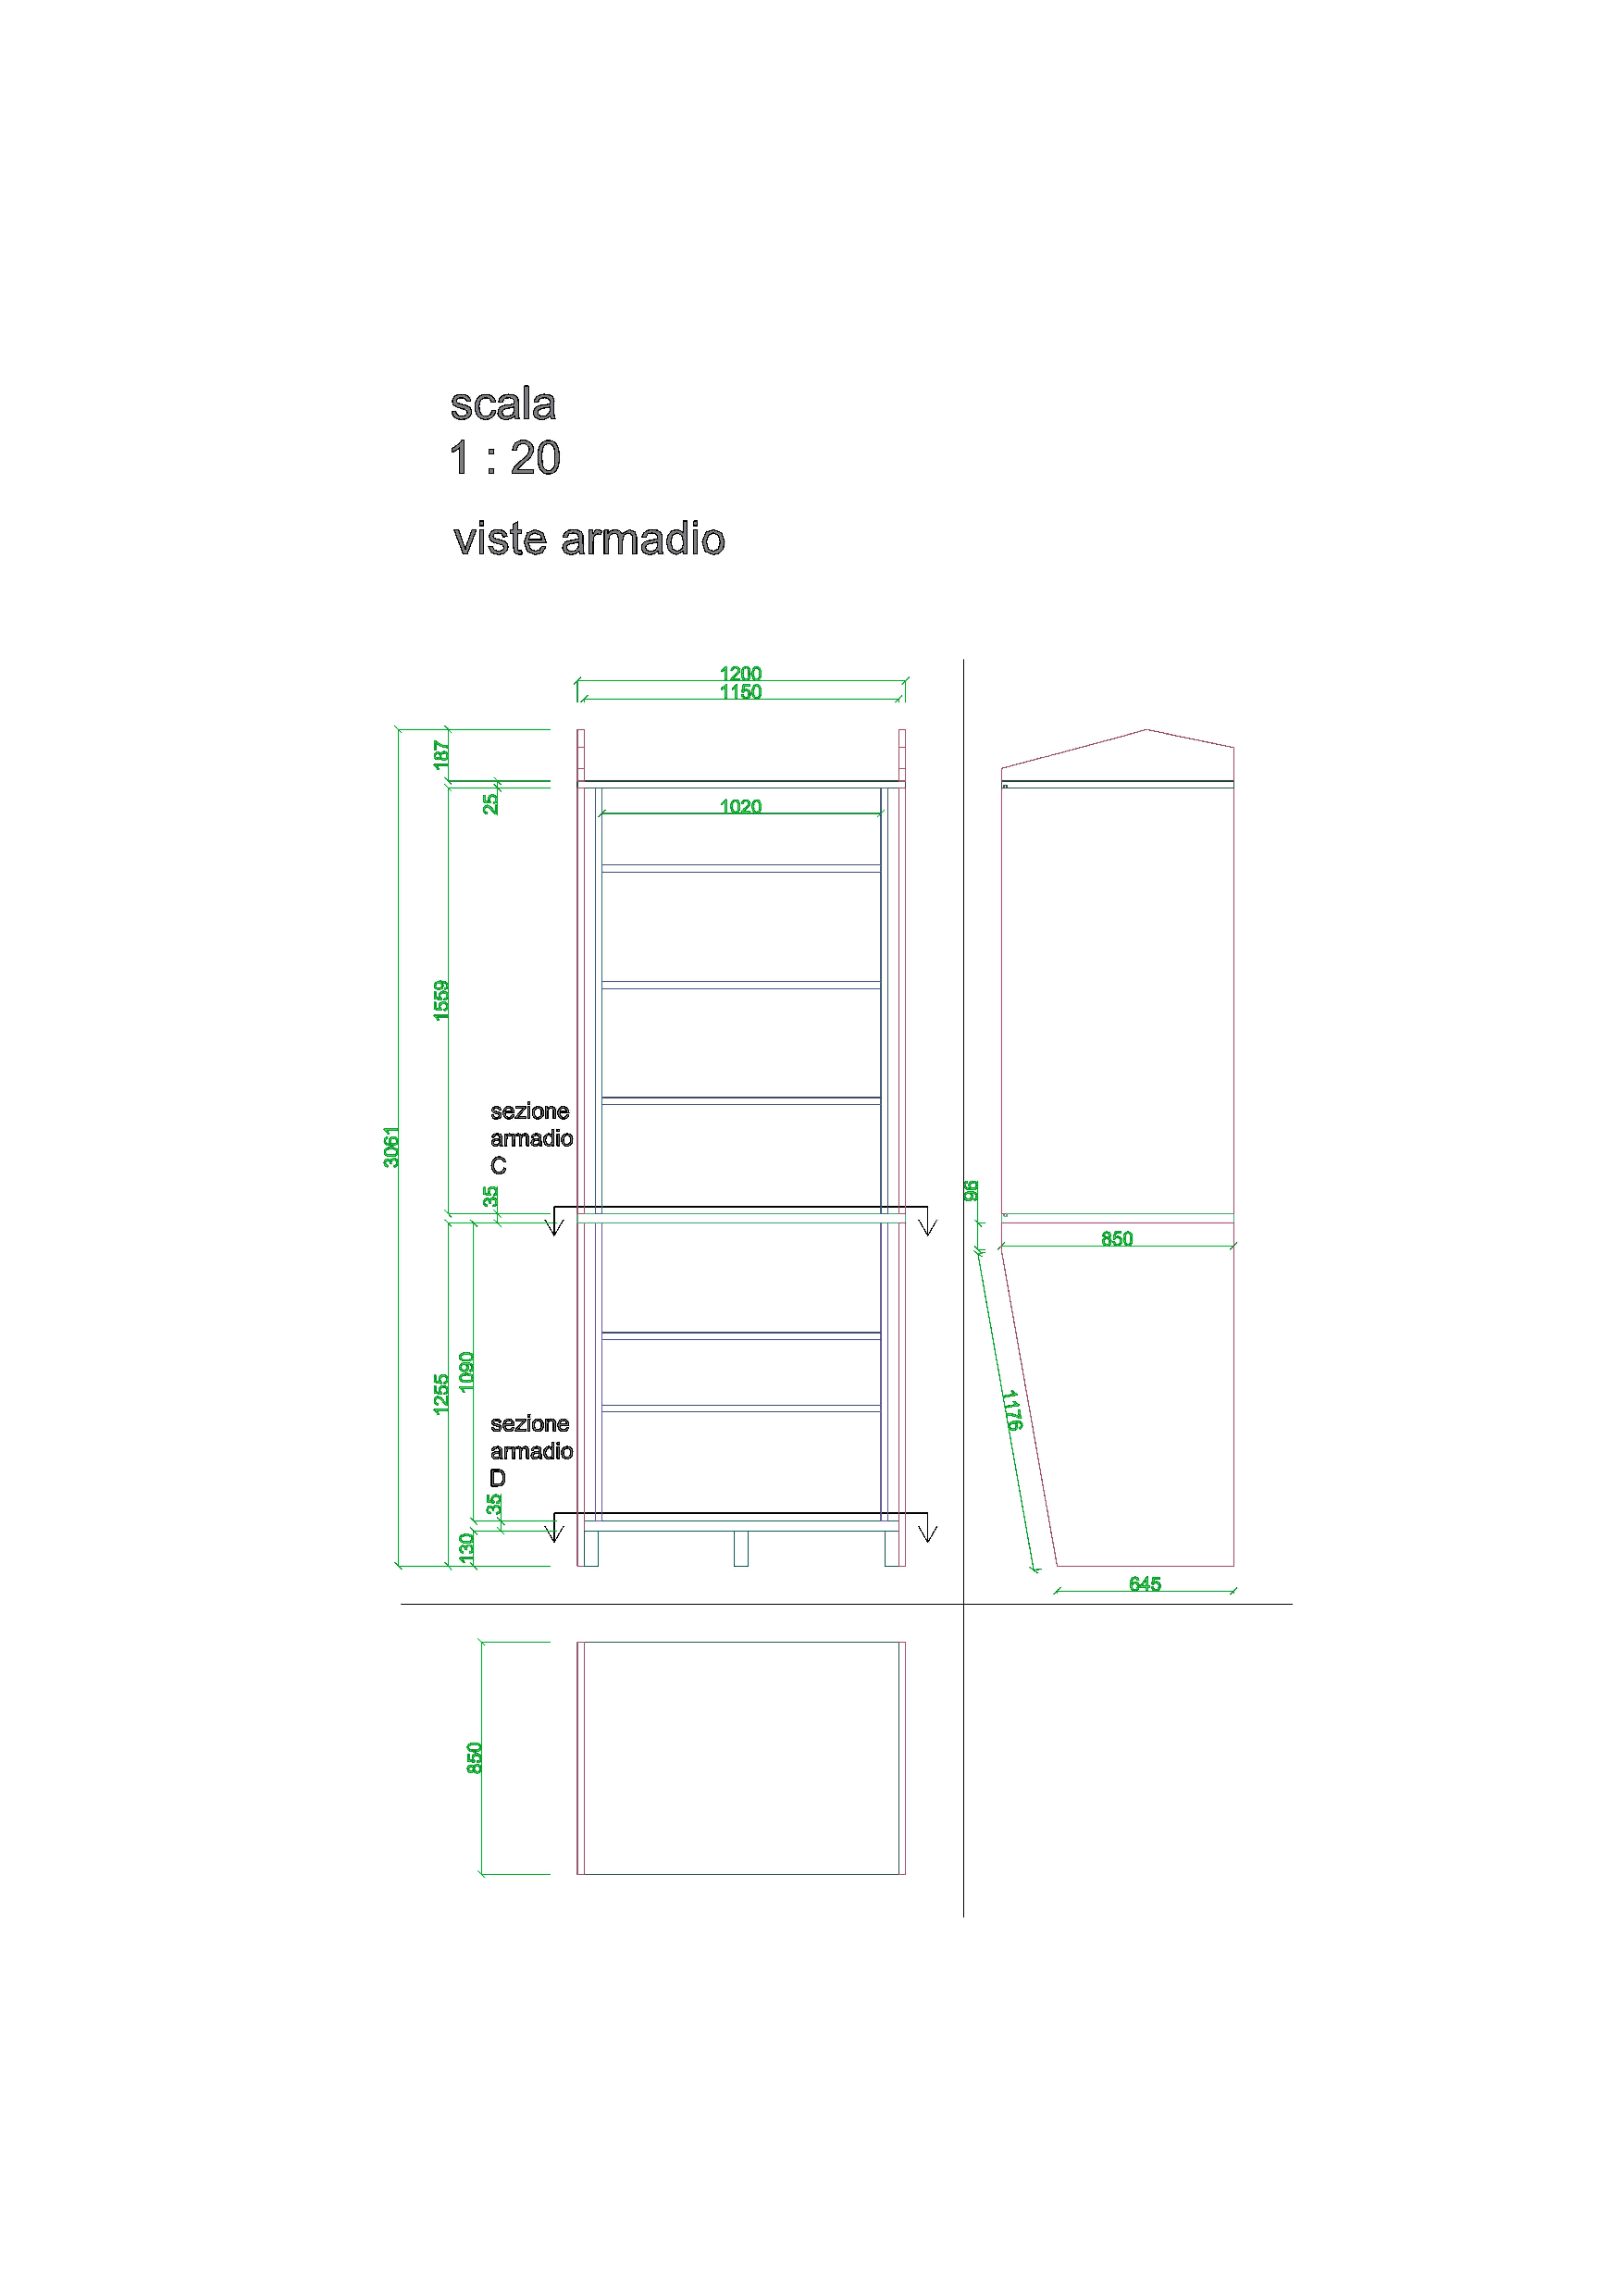
\includegraphics[width=1\linewidth]{35}
\end{figure}

\begin{figure}[H]
	\centering
	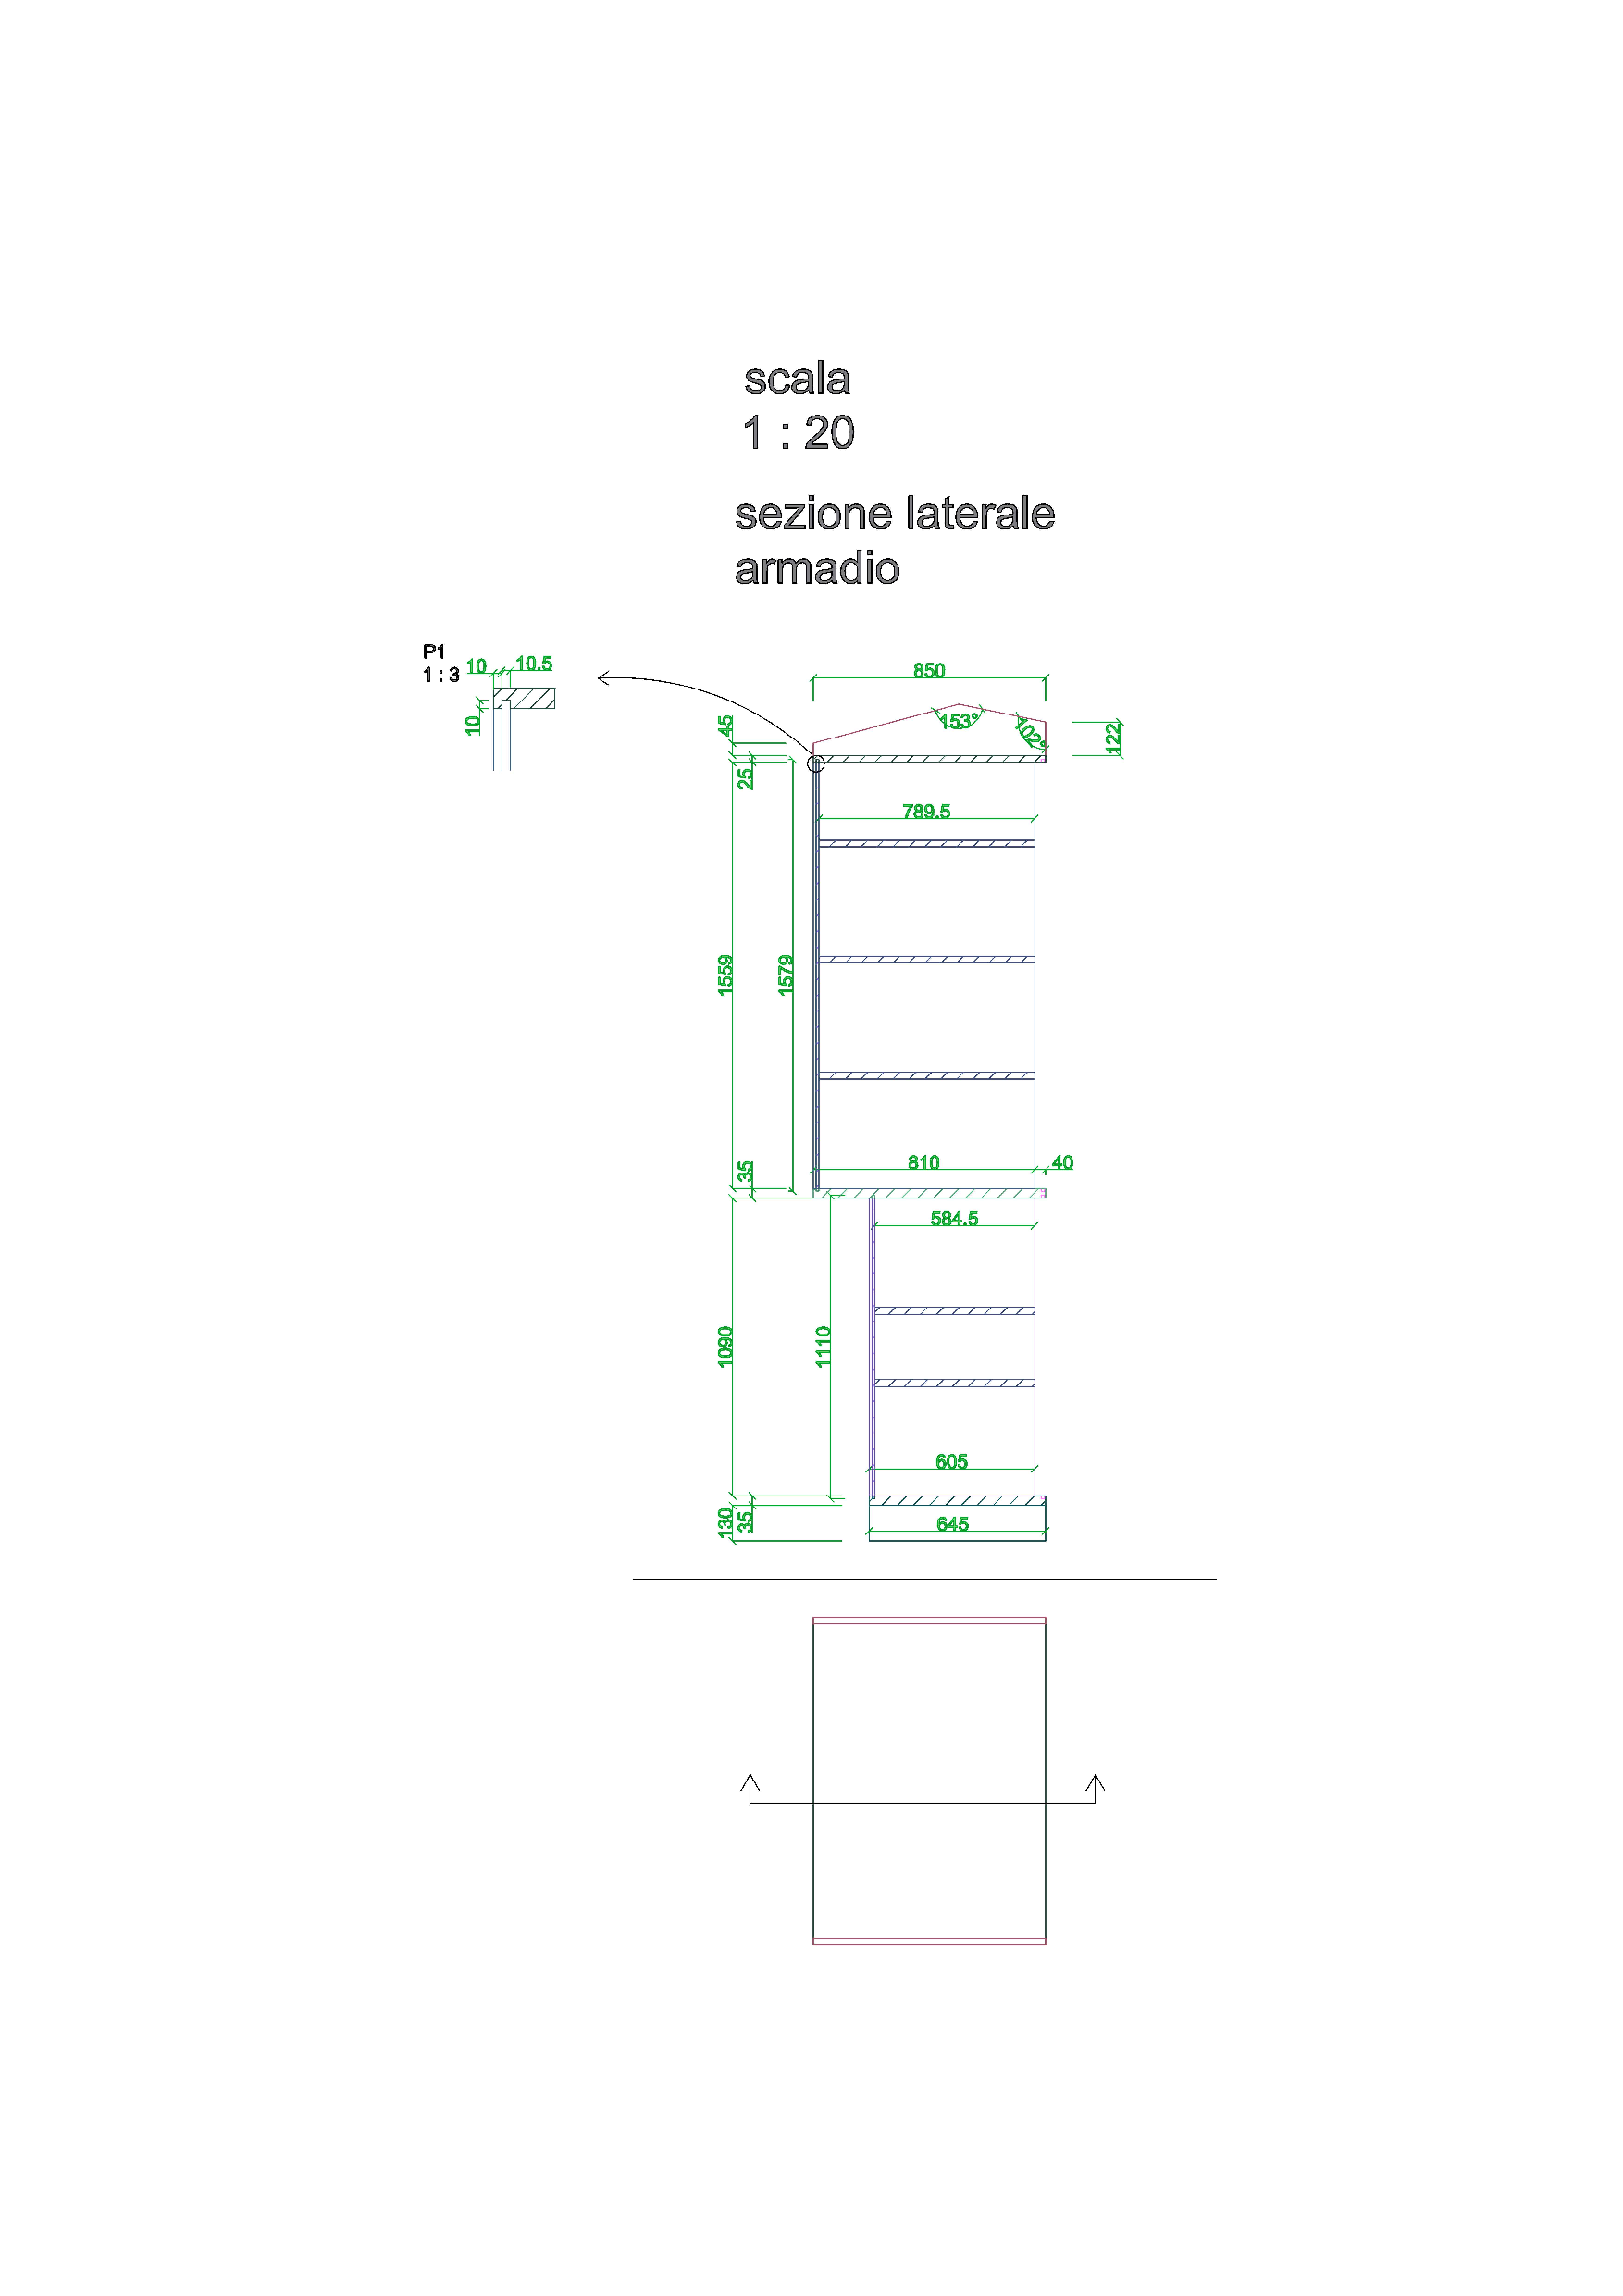
\includegraphics[width=1\linewidth]{36}
\end{figure}

\begin{figure}[H]
	\centering
	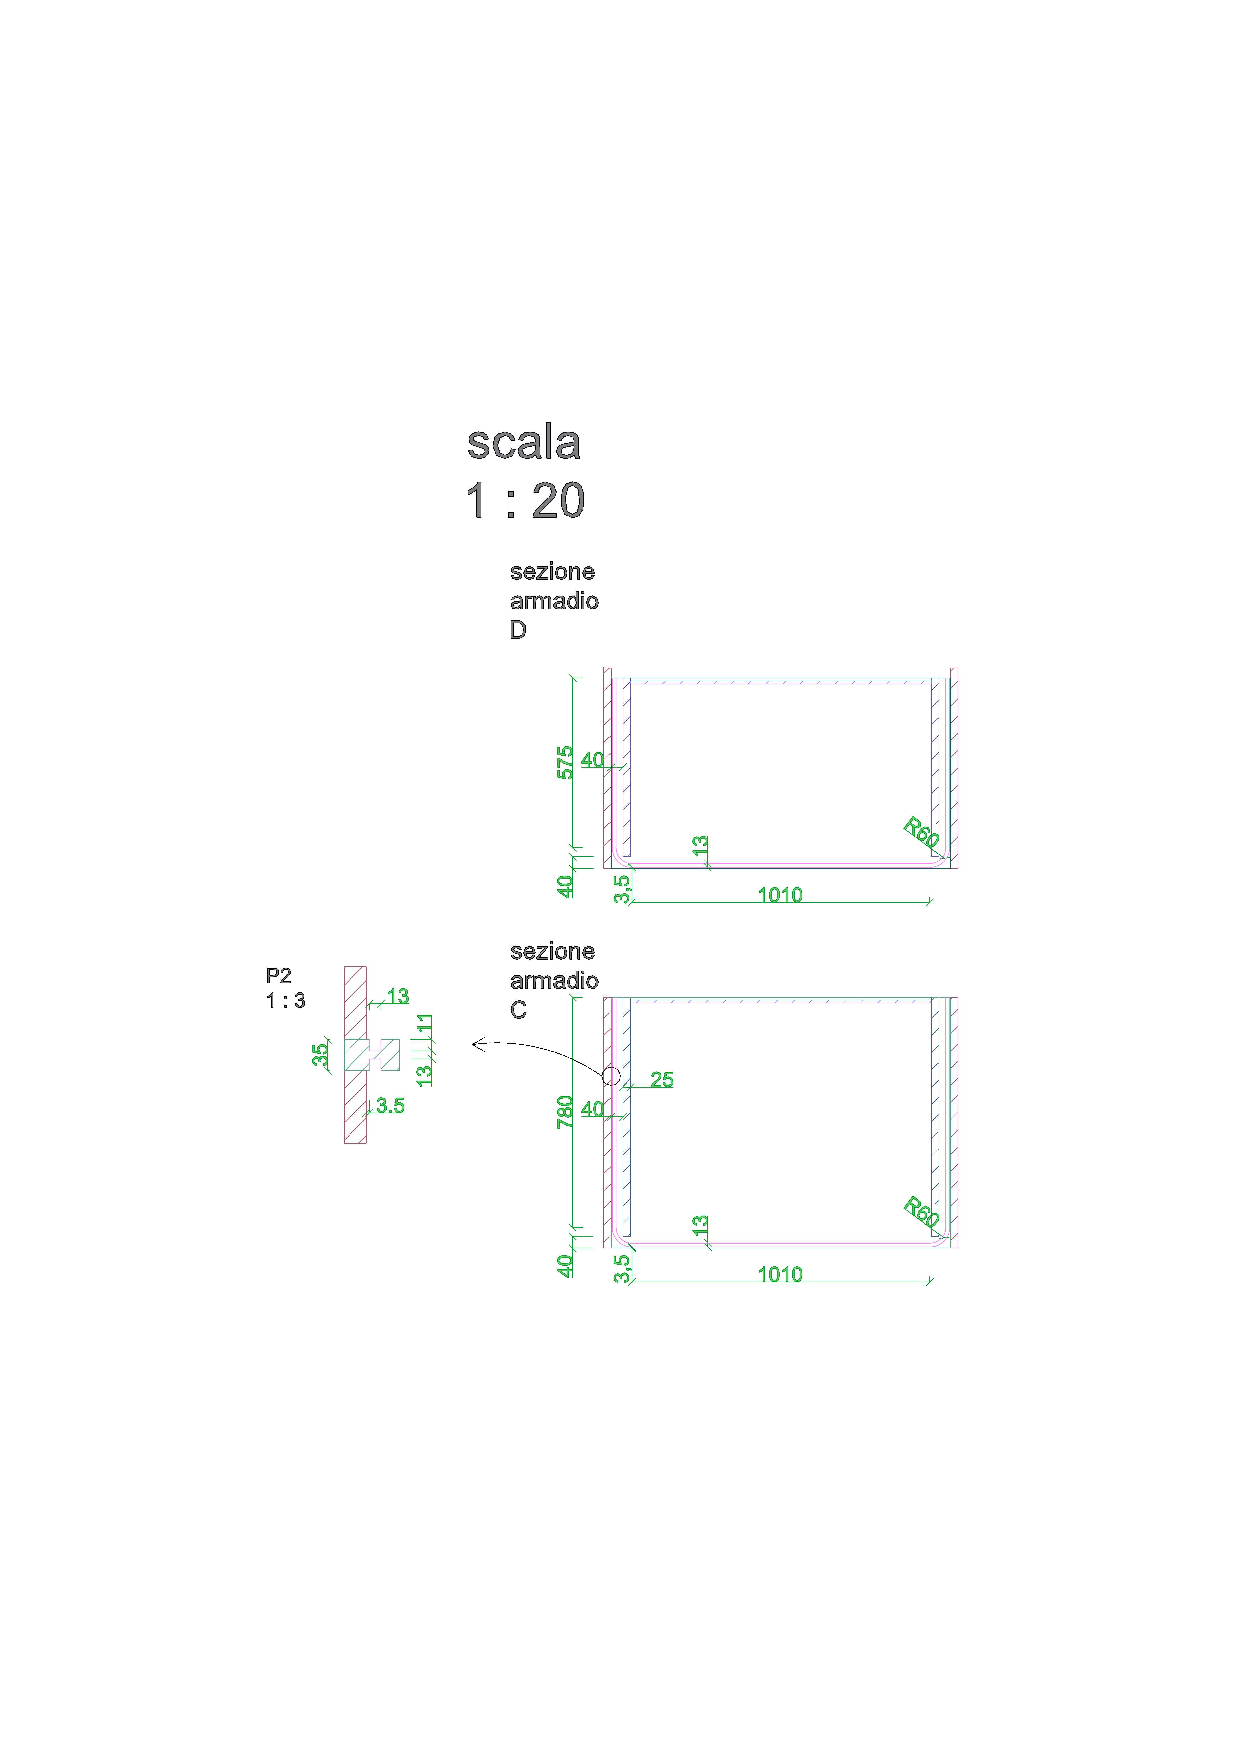
\includegraphics[width=1\linewidth]{37}
\end{figure}

\begin{figure}[H]
	\centering
	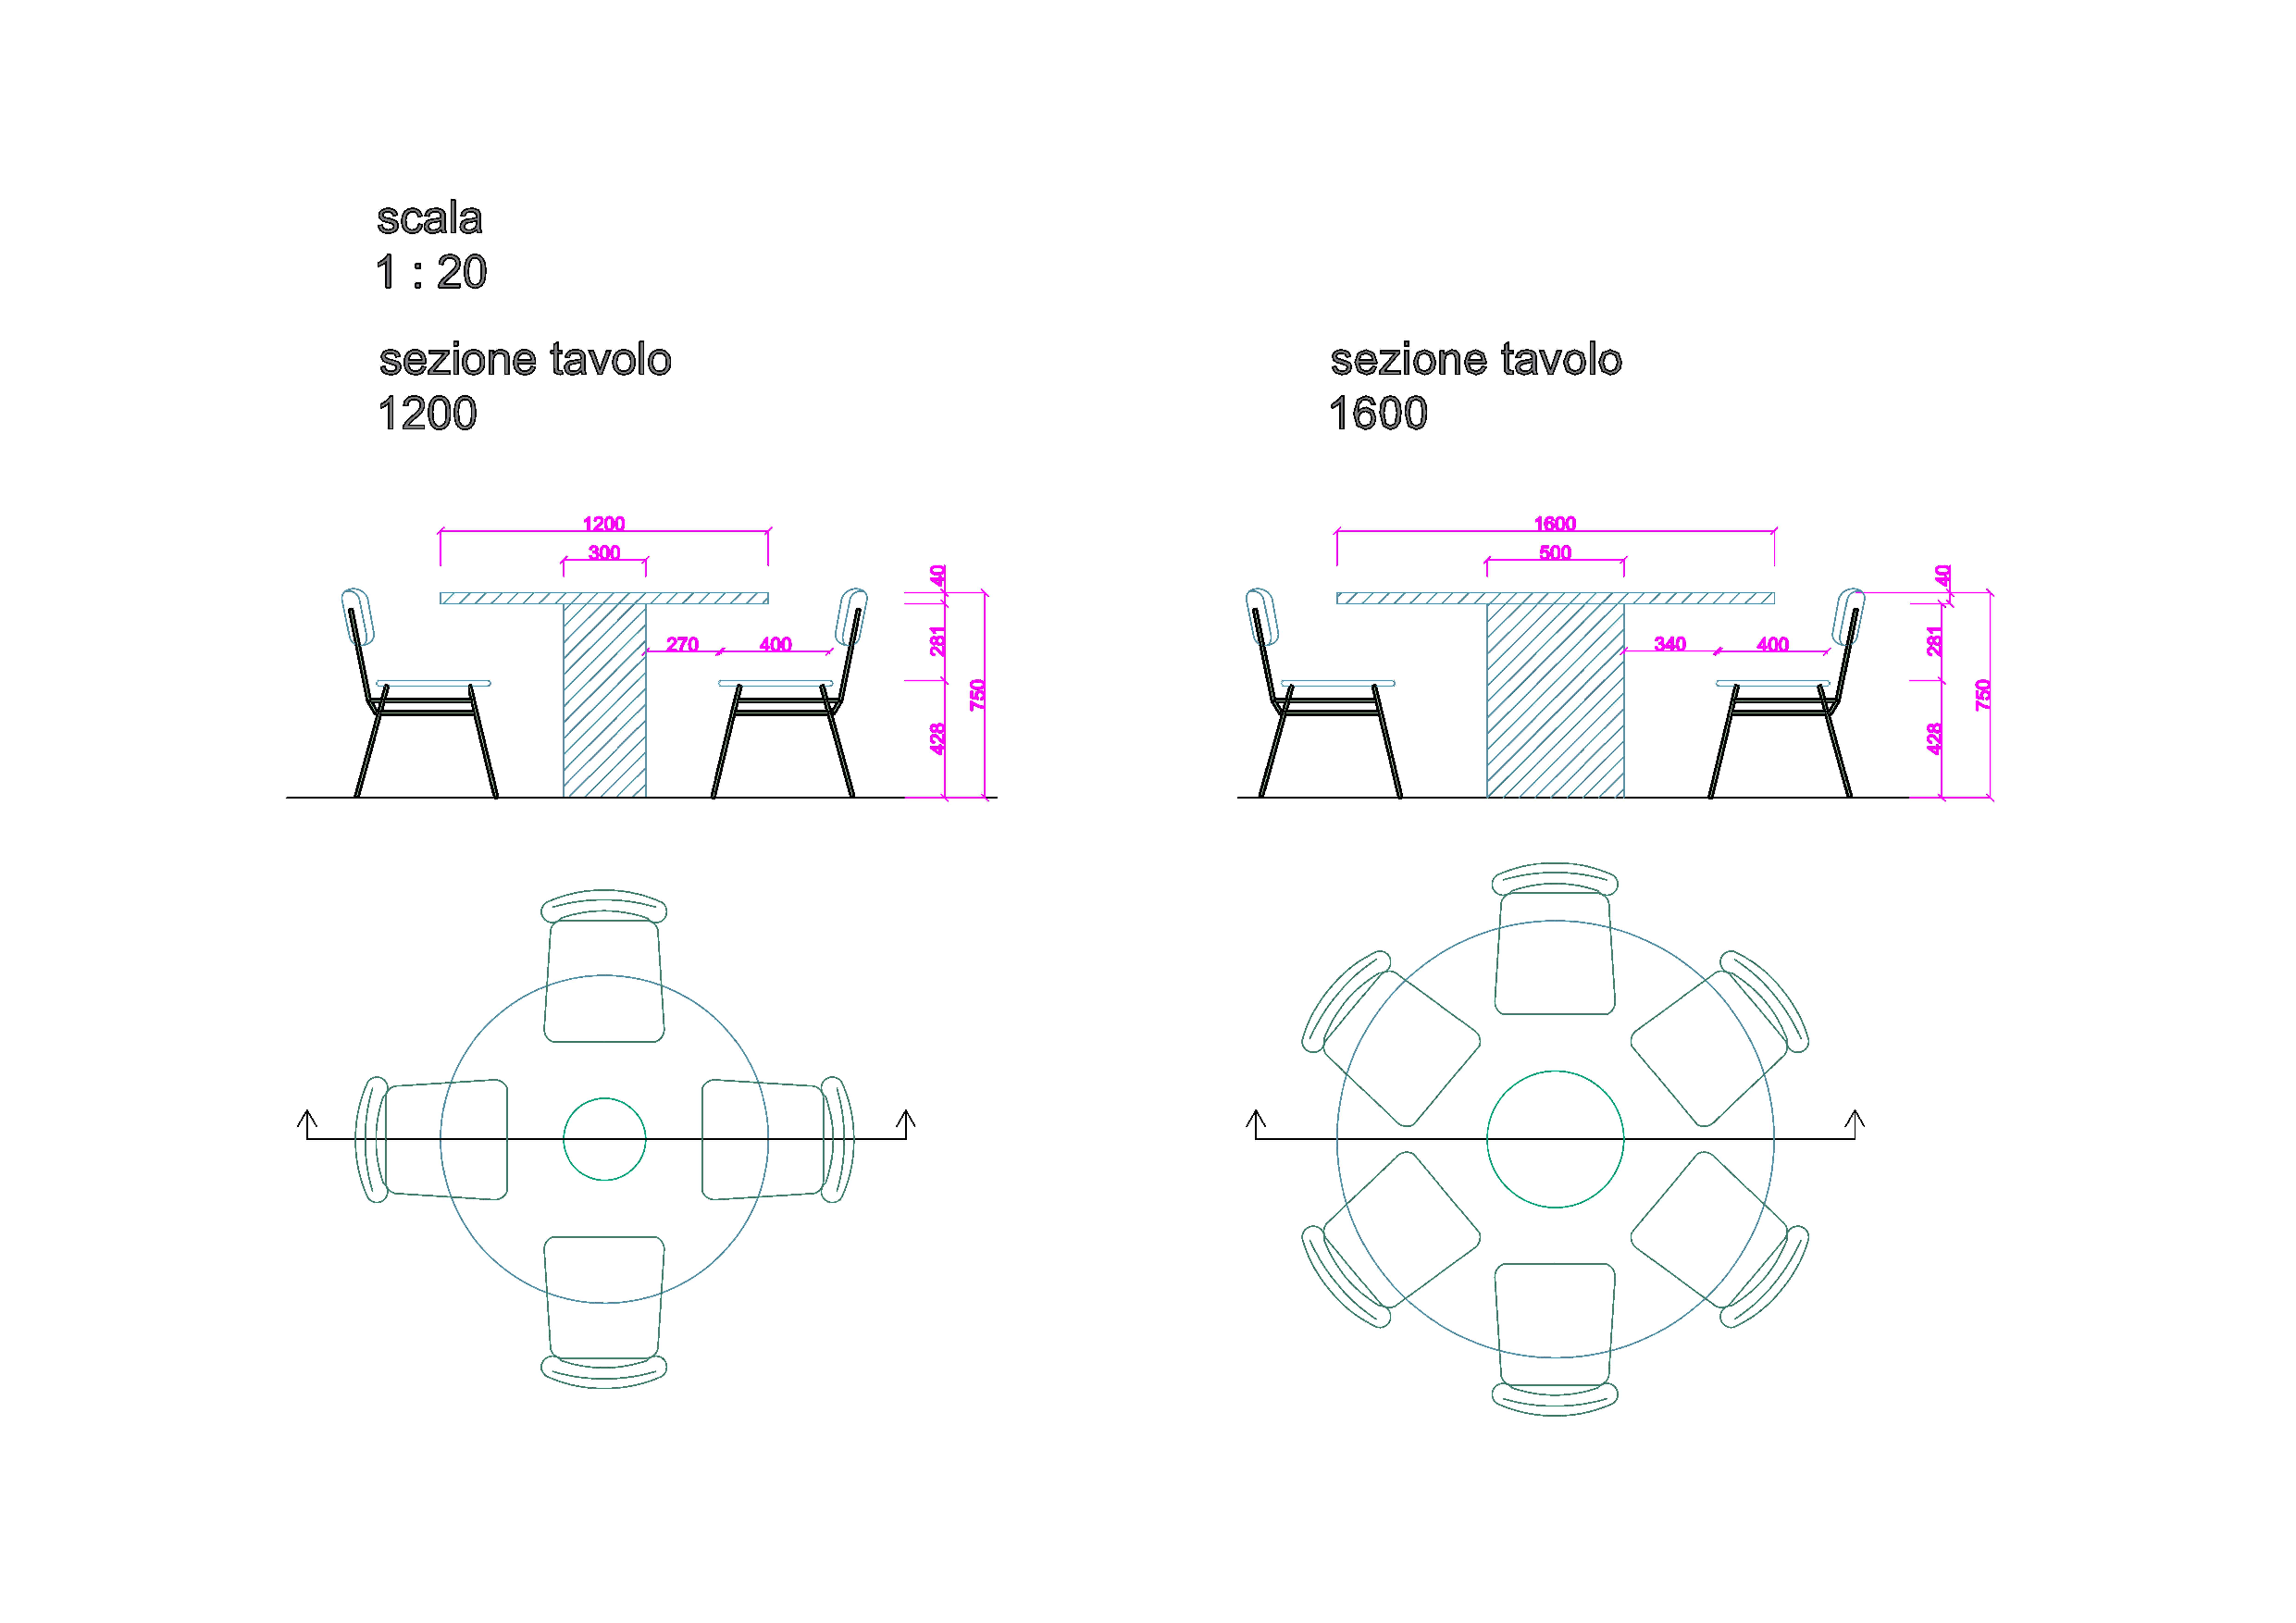
\includegraphics[width=1\linewidth]{38}
\end{figure}

\begin{figure}[H]
	\centering
	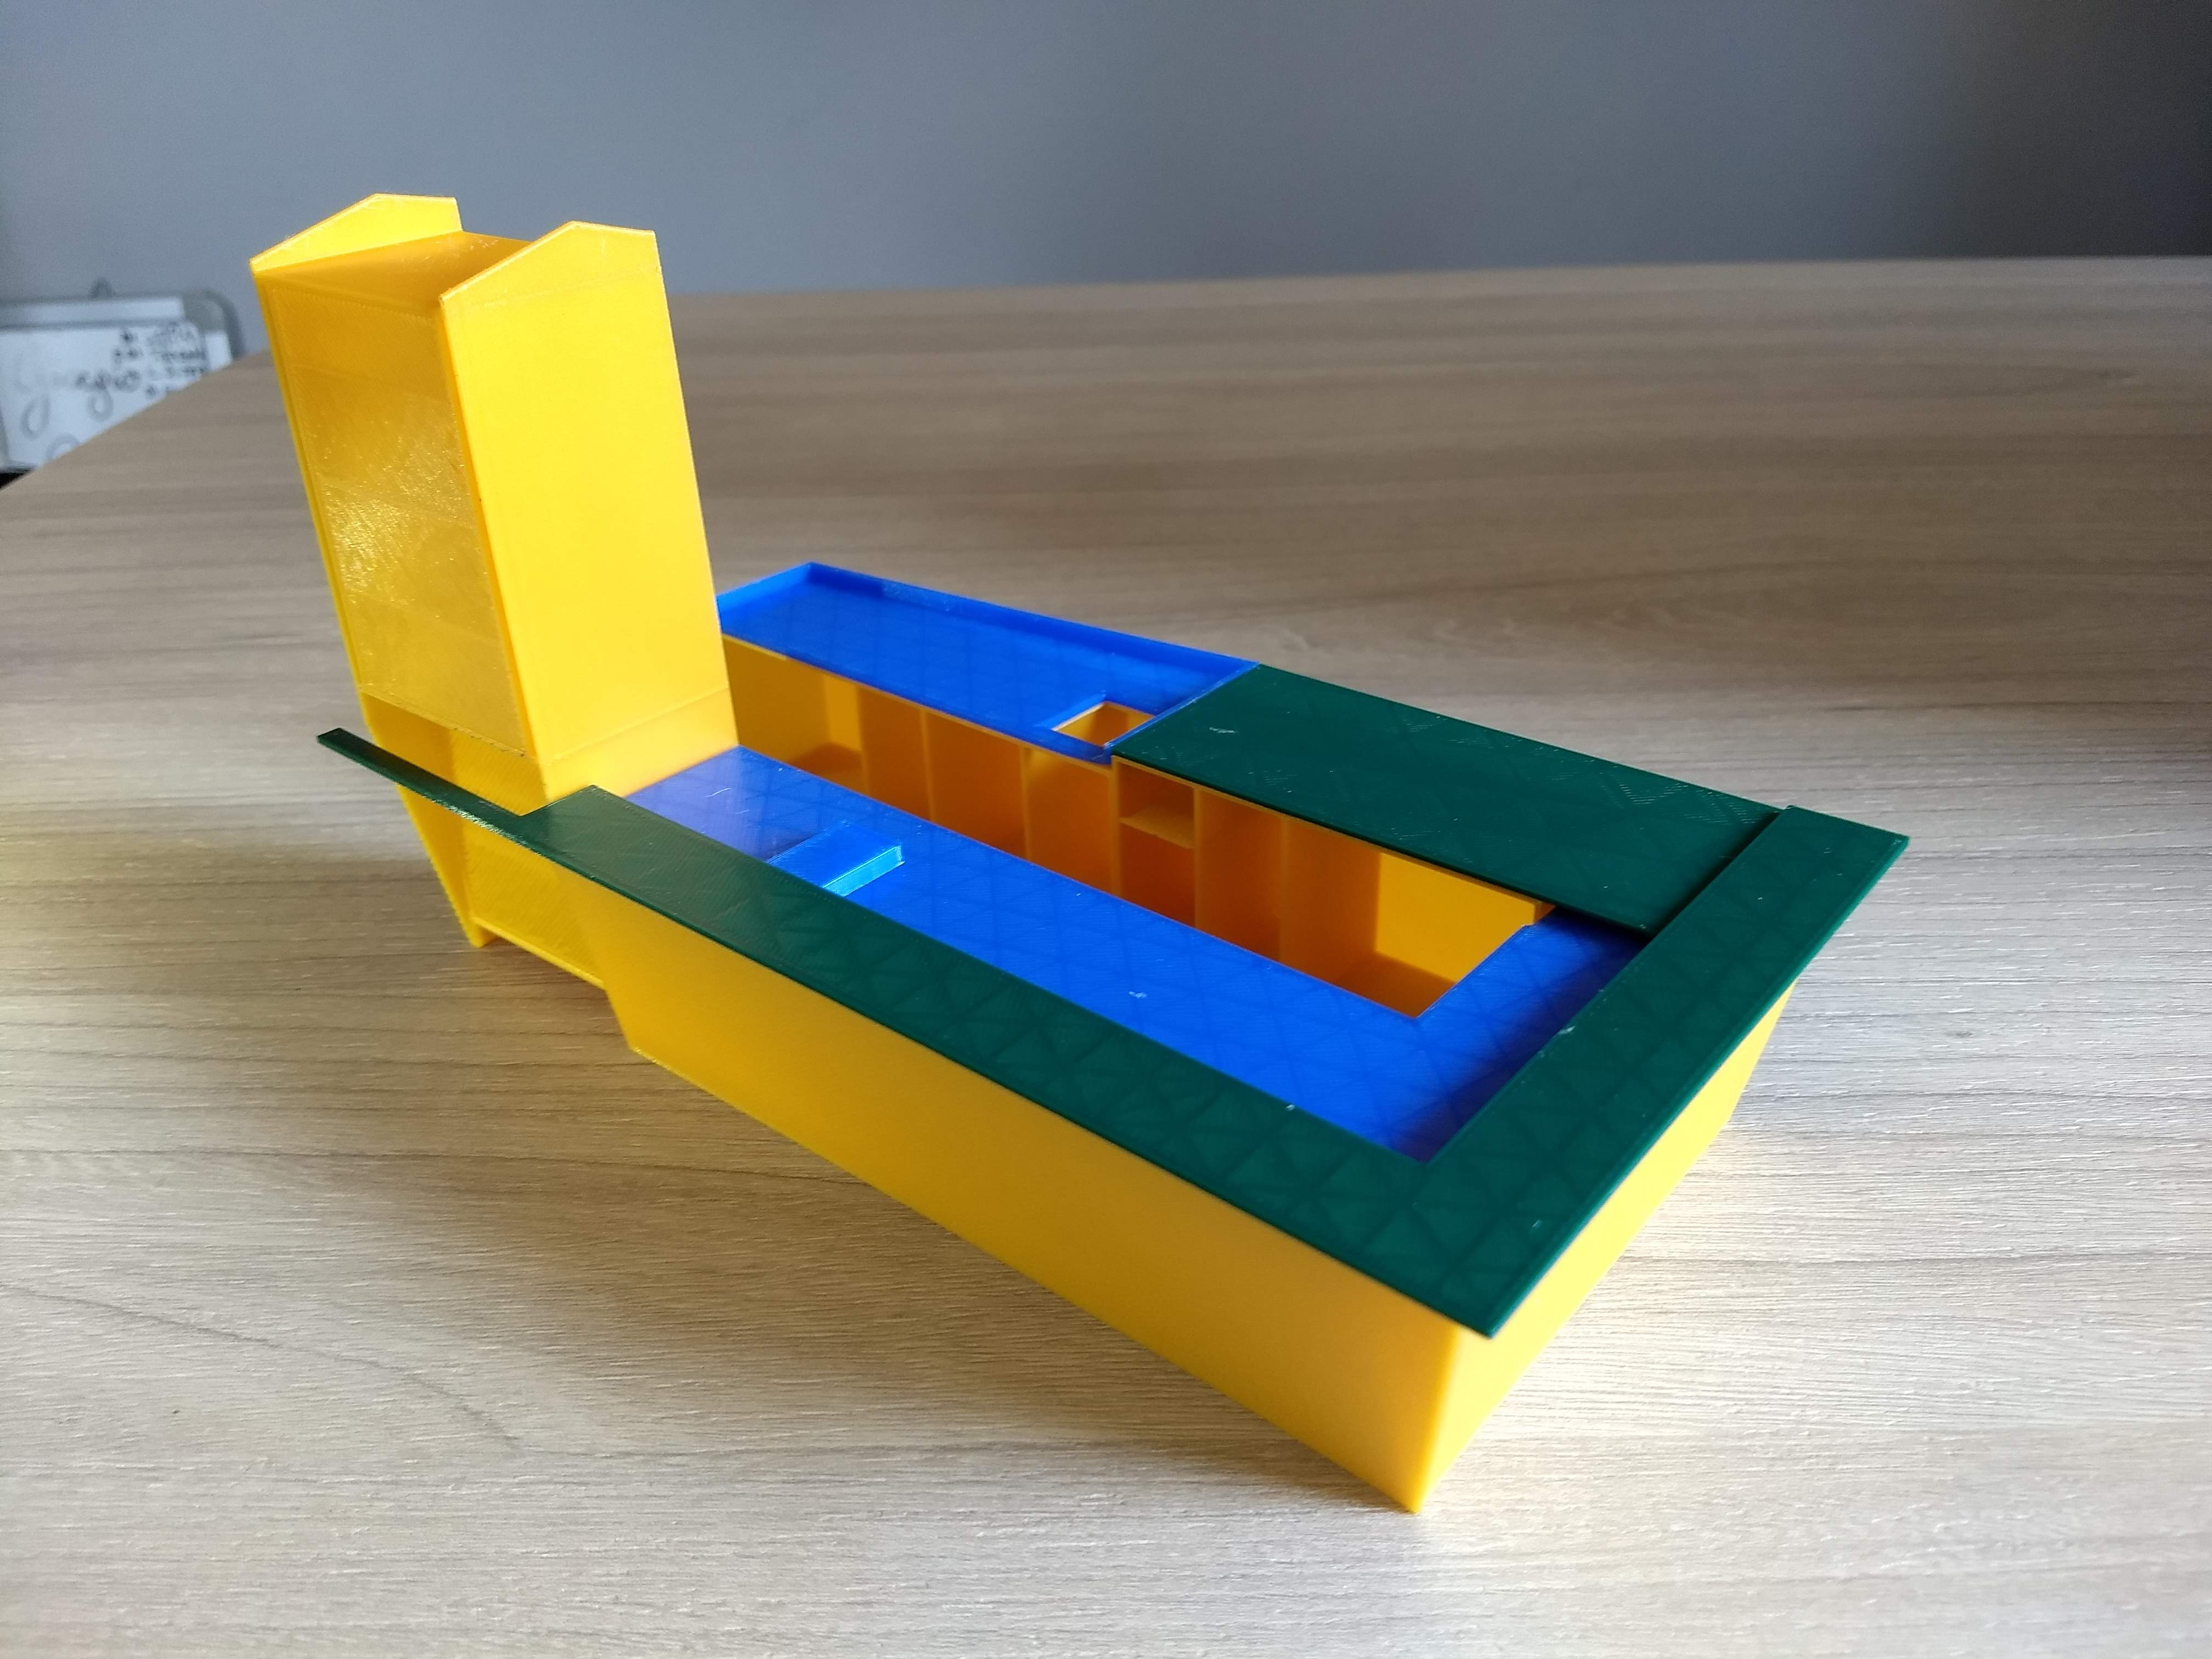
\includegraphics[width=1\linewidth]{39}
\end{figure}

% -------------------------------------------

\begin{figure}[H]
	\centering
	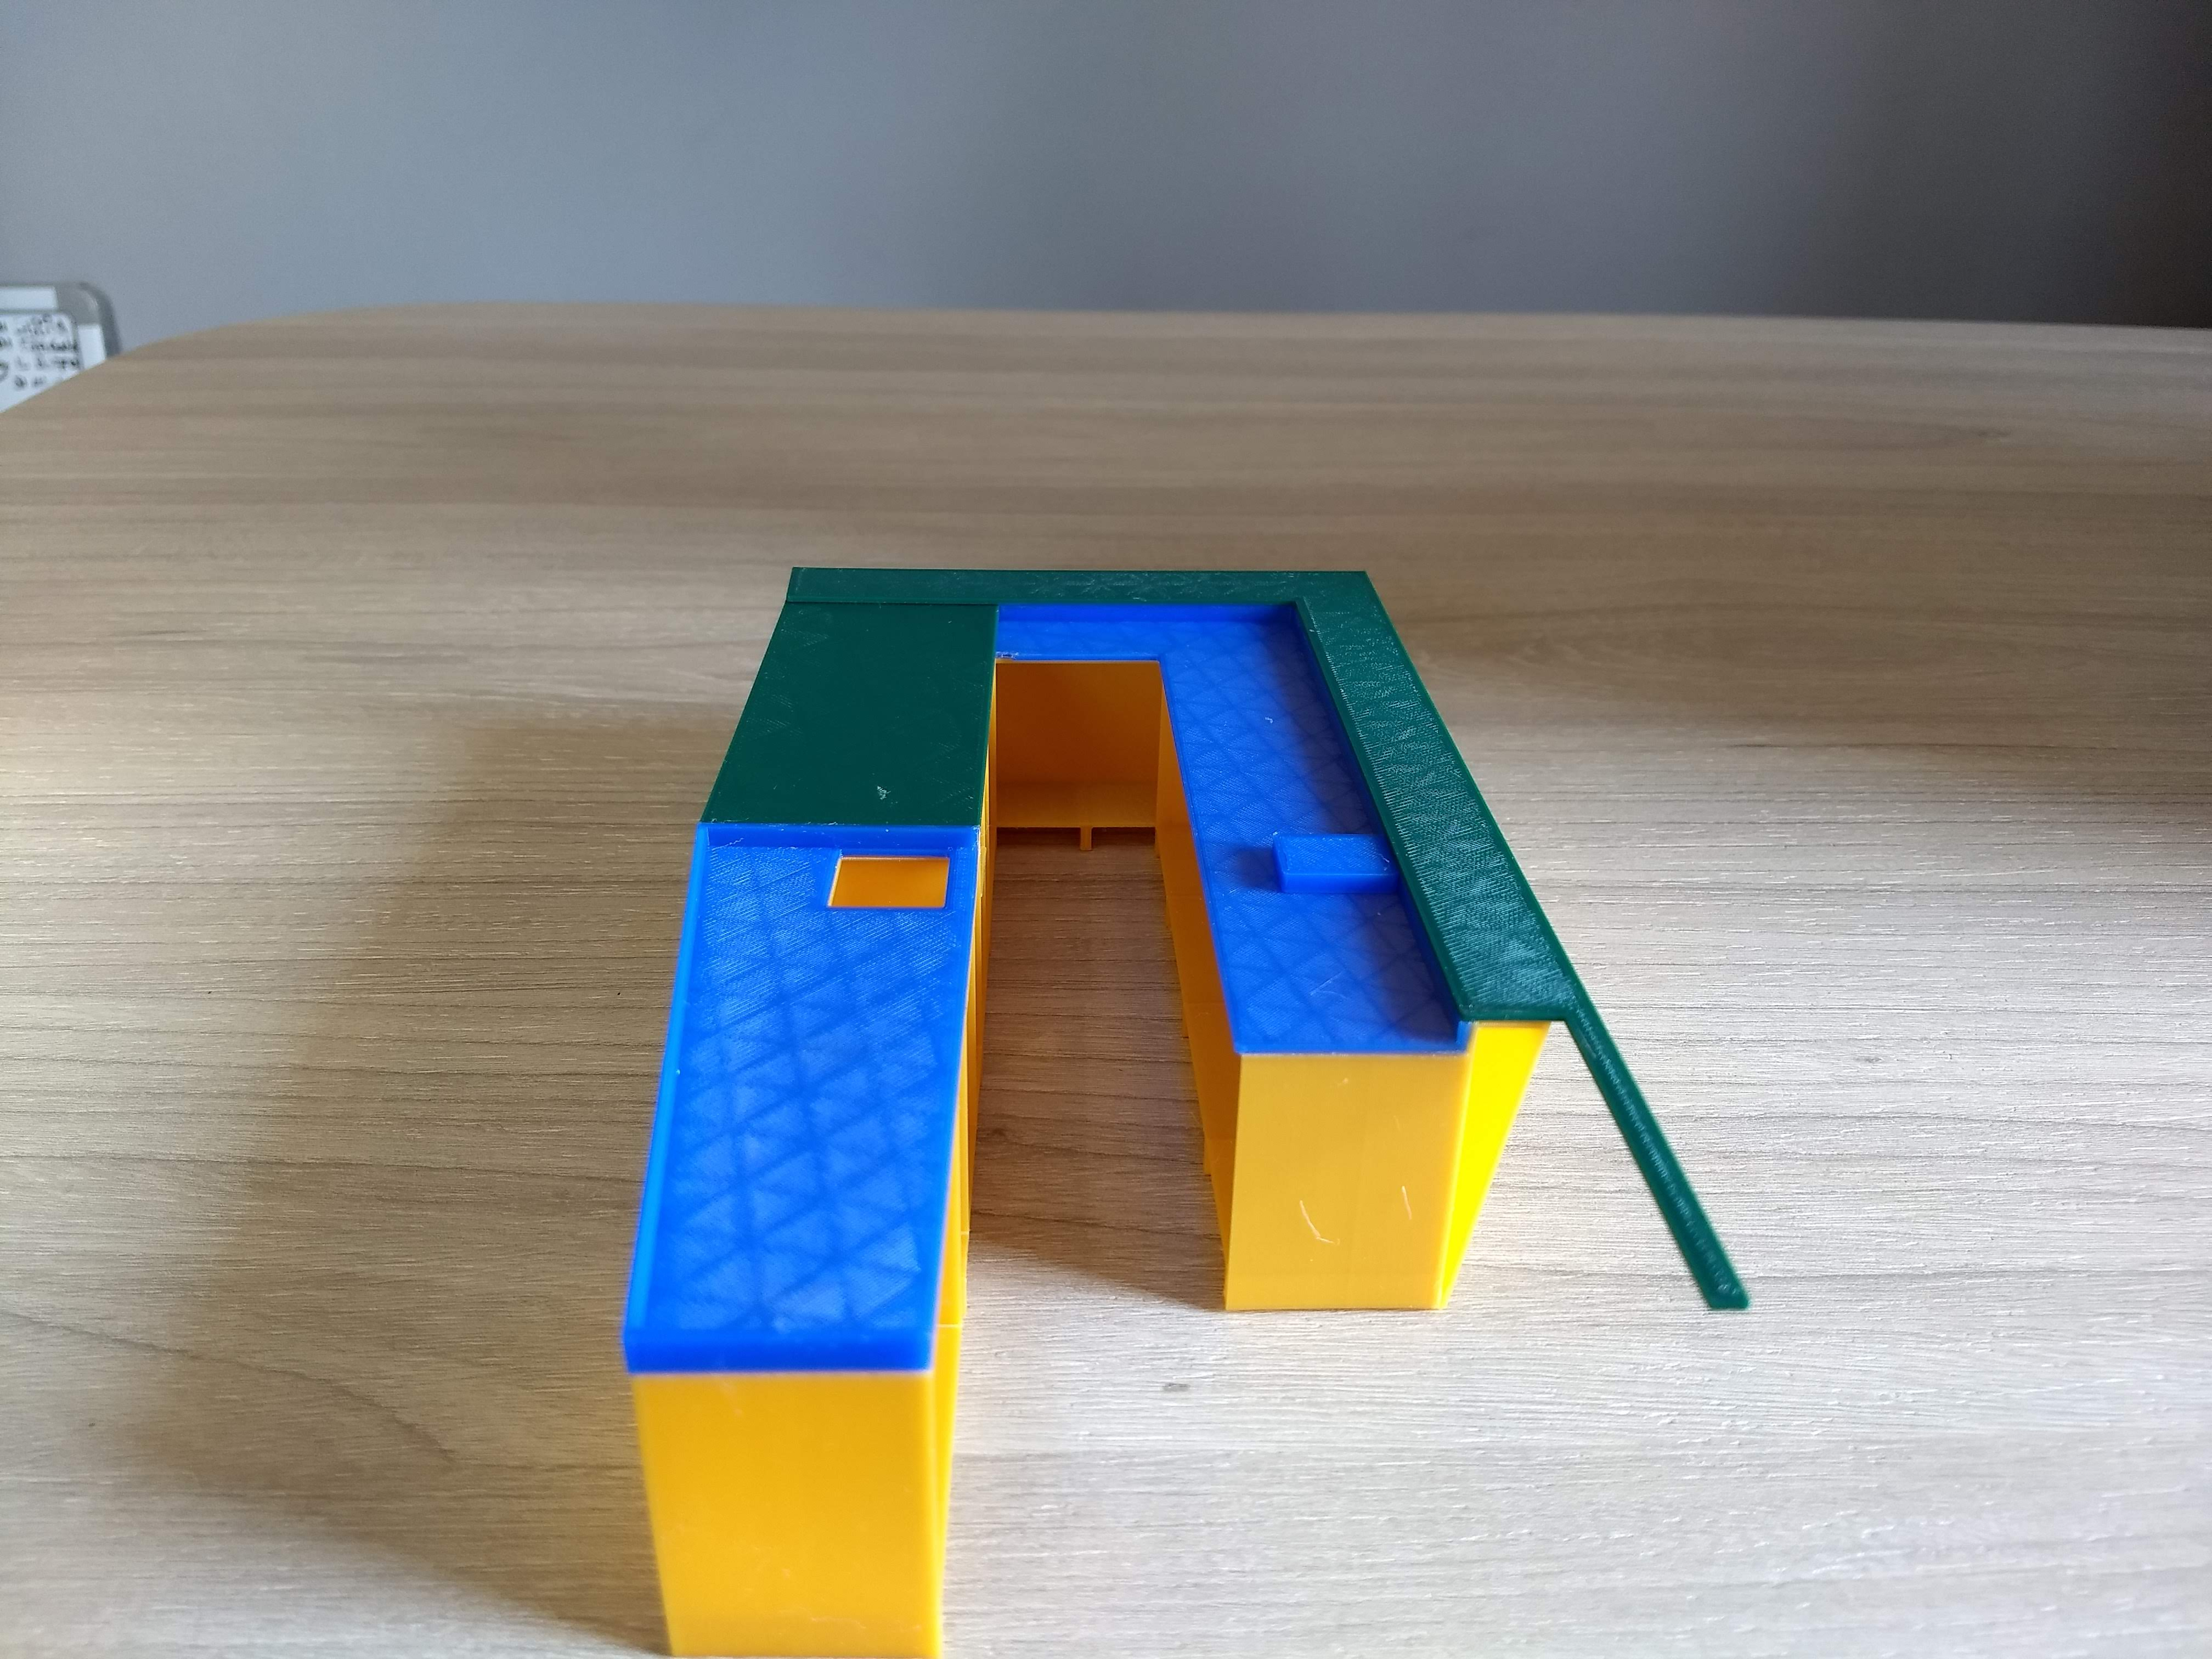
\includegraphics[width=1\linewidth]{40}
\end{figure}

\begin{figure}[H]
	\centering
	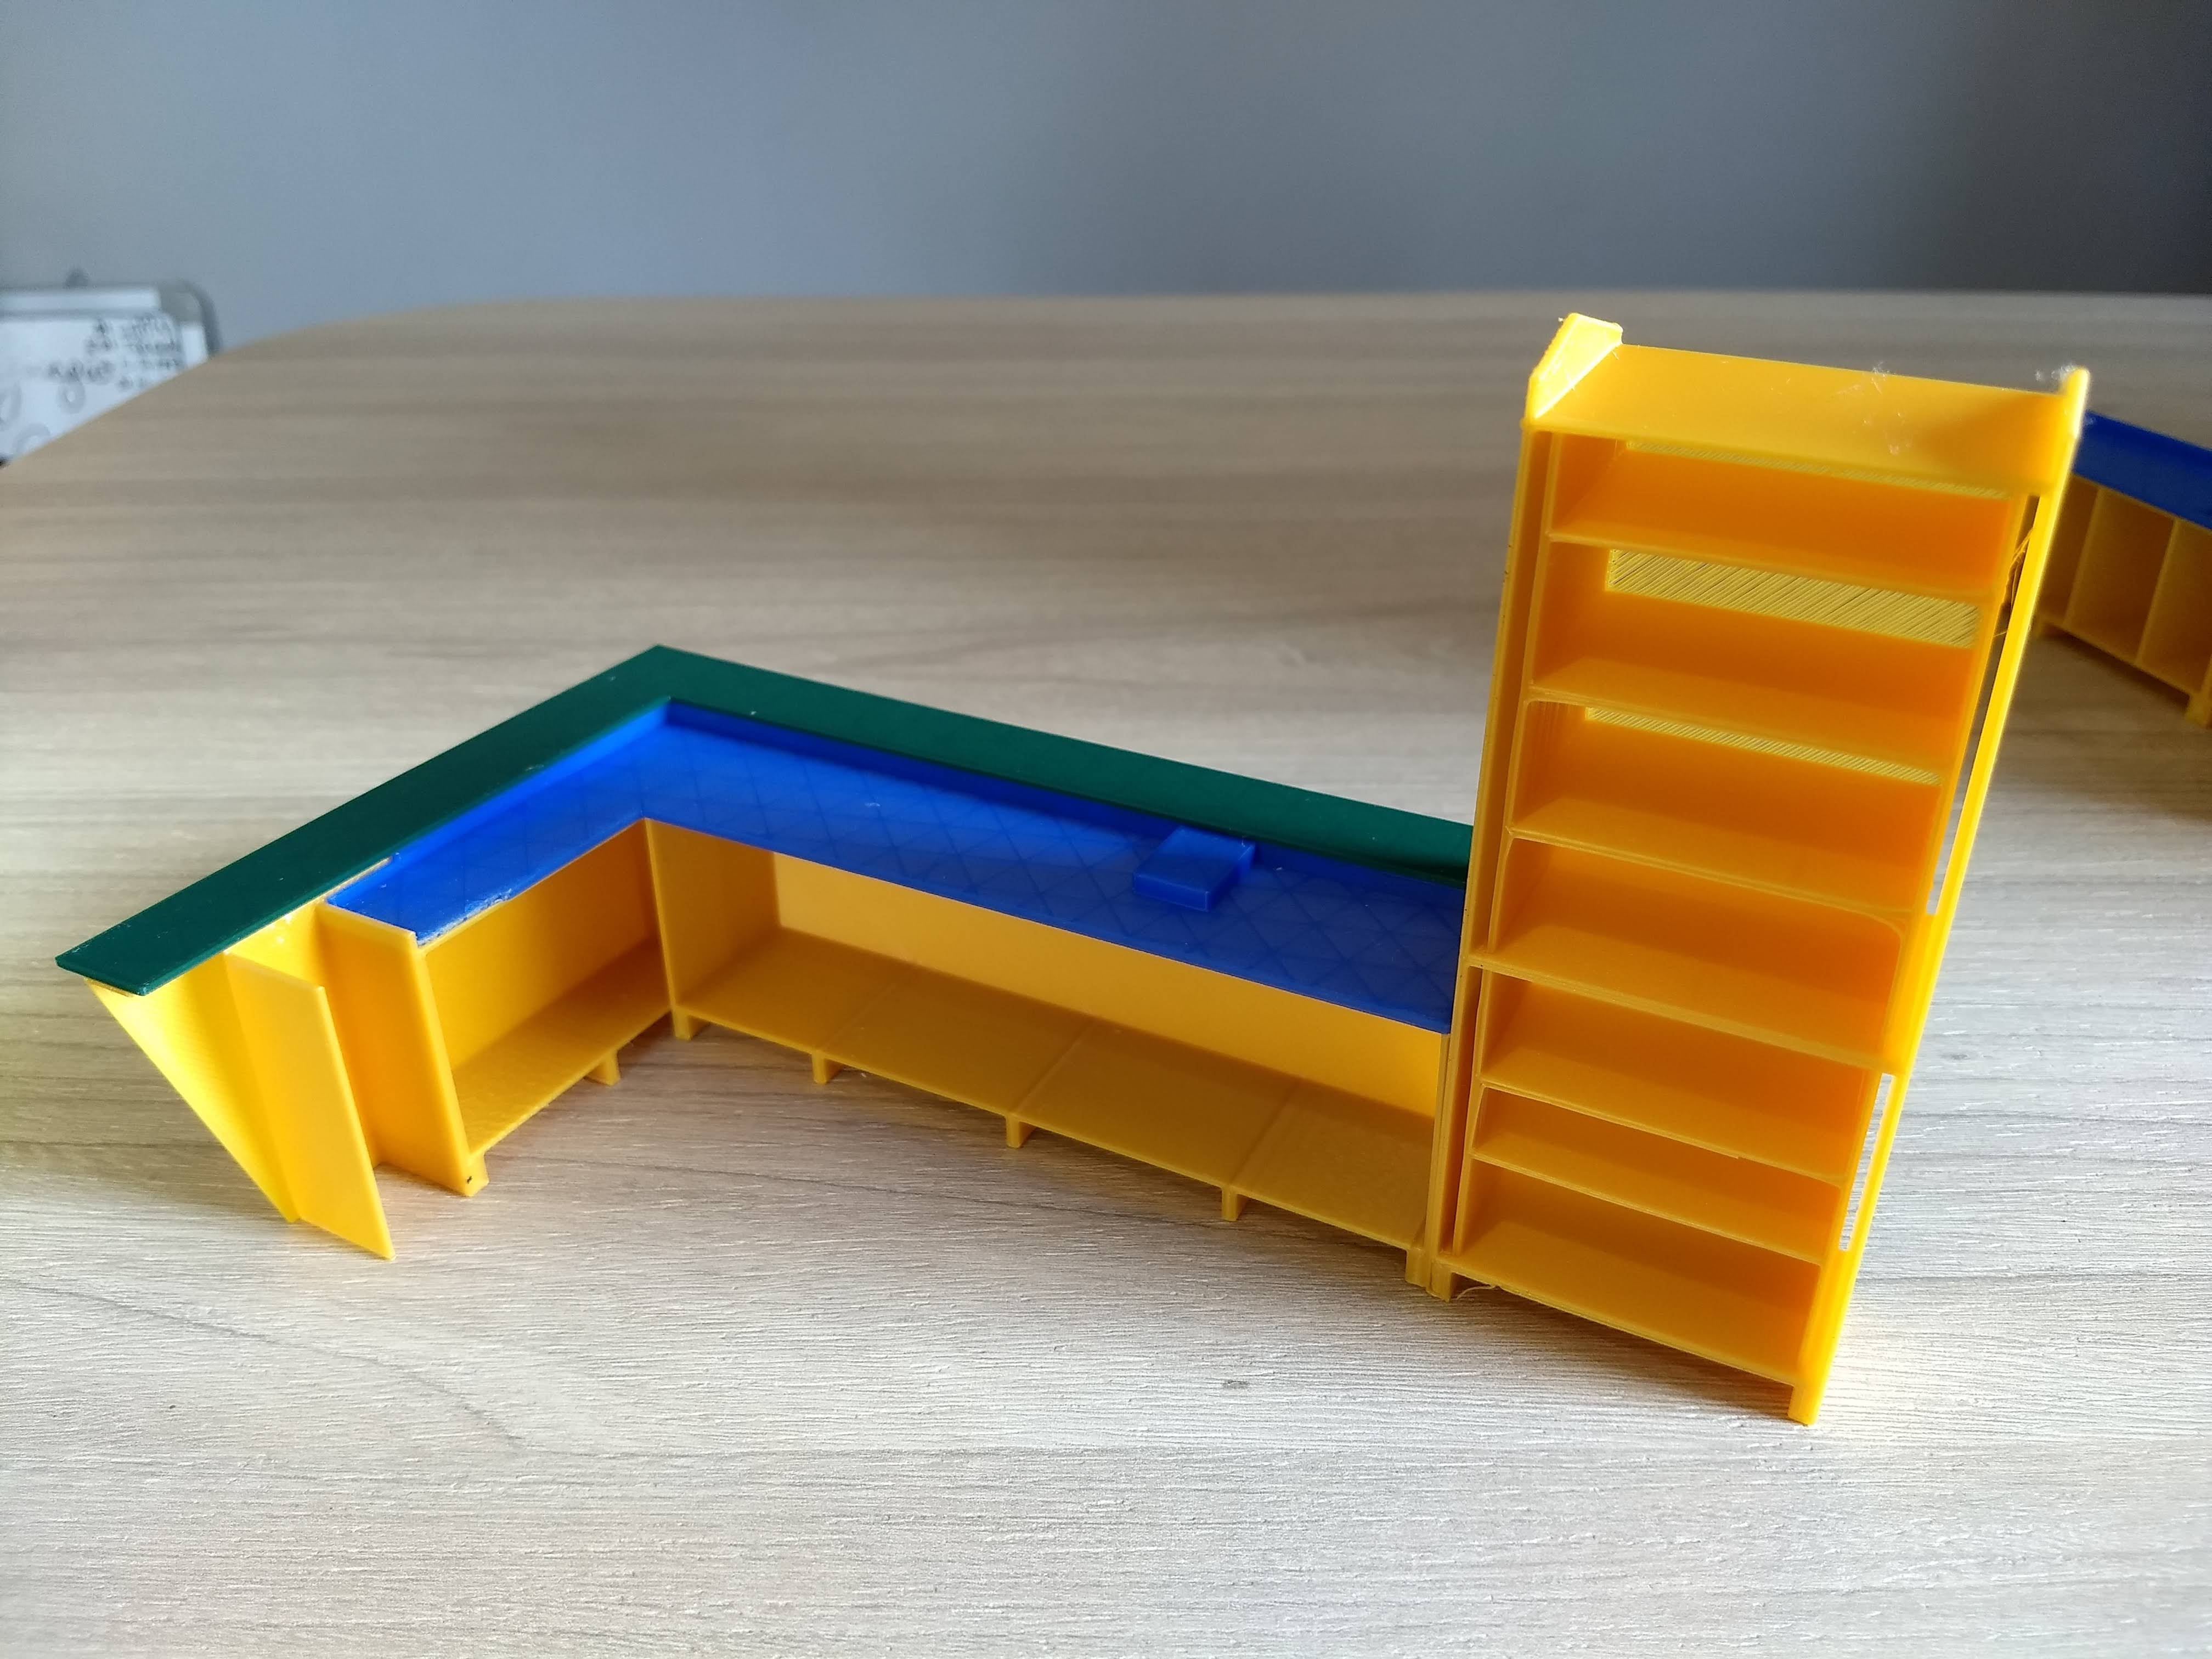
\includegraphics[width=1\linewidth]{41}
\end{figure}

\begin{figure}[H]
	\centering
	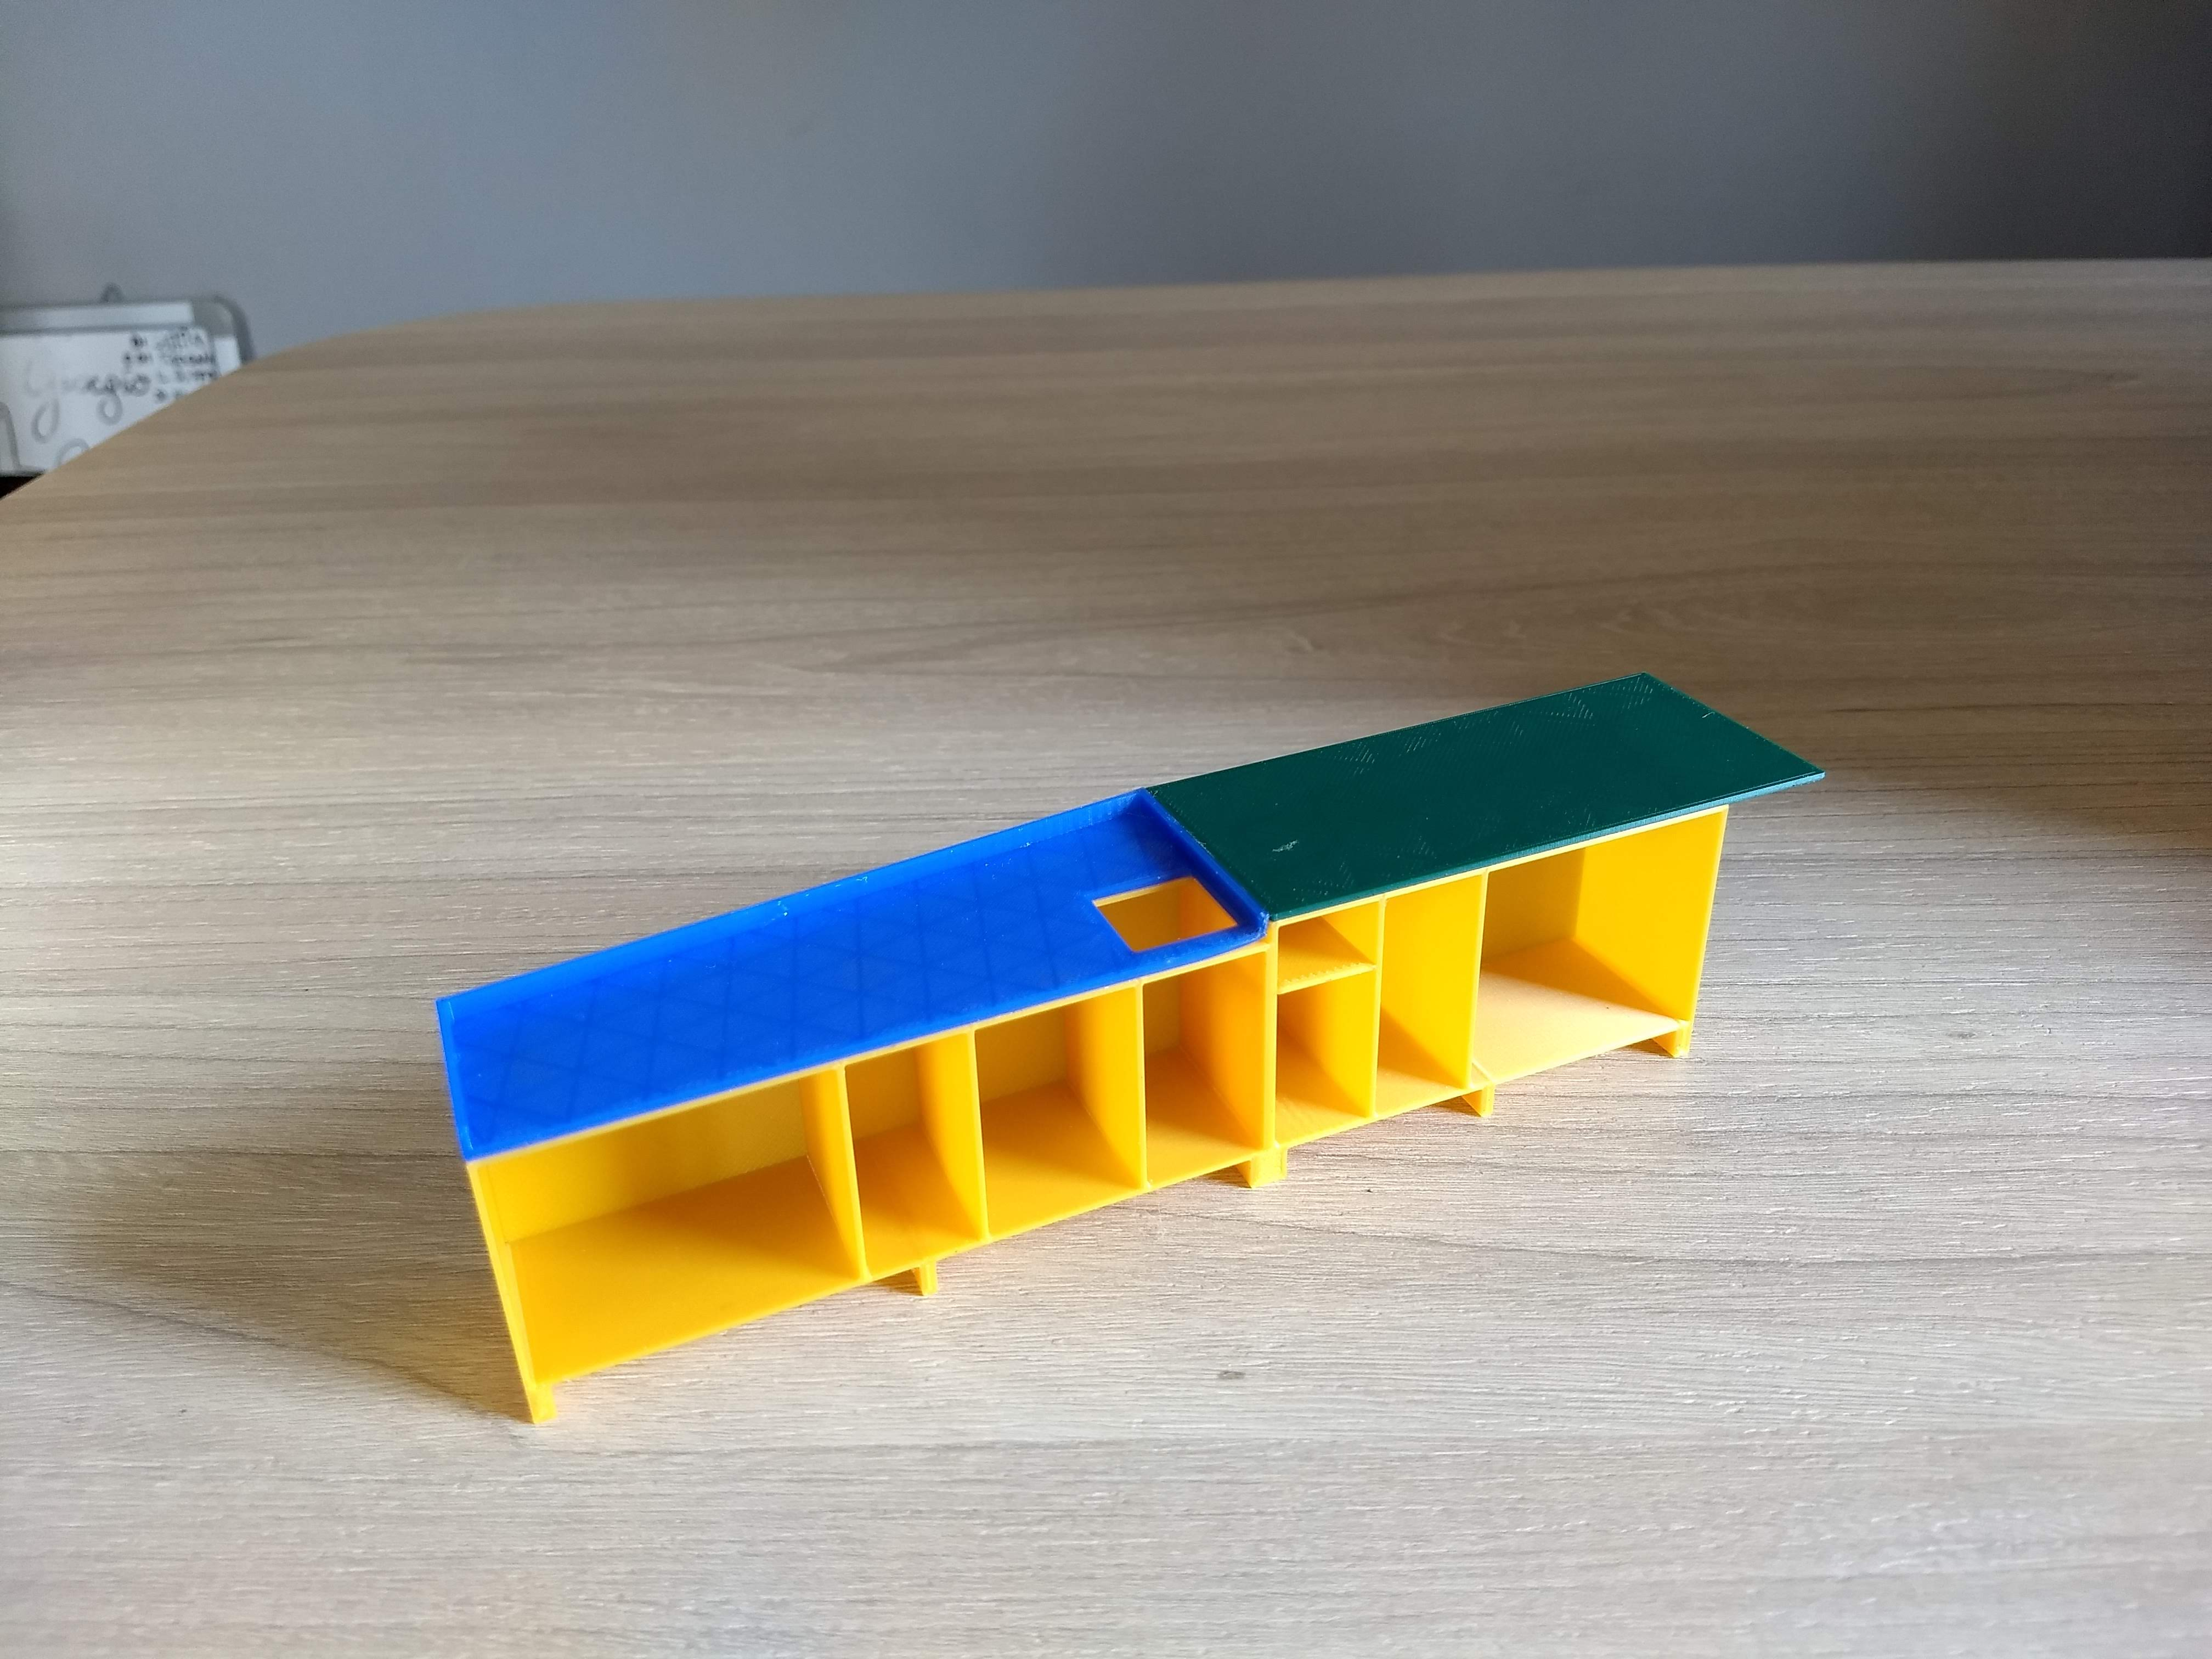
\includegraphics[width=1\linewidth]{42}
\end{figure}

\begin{figure}[H]
	\centering
	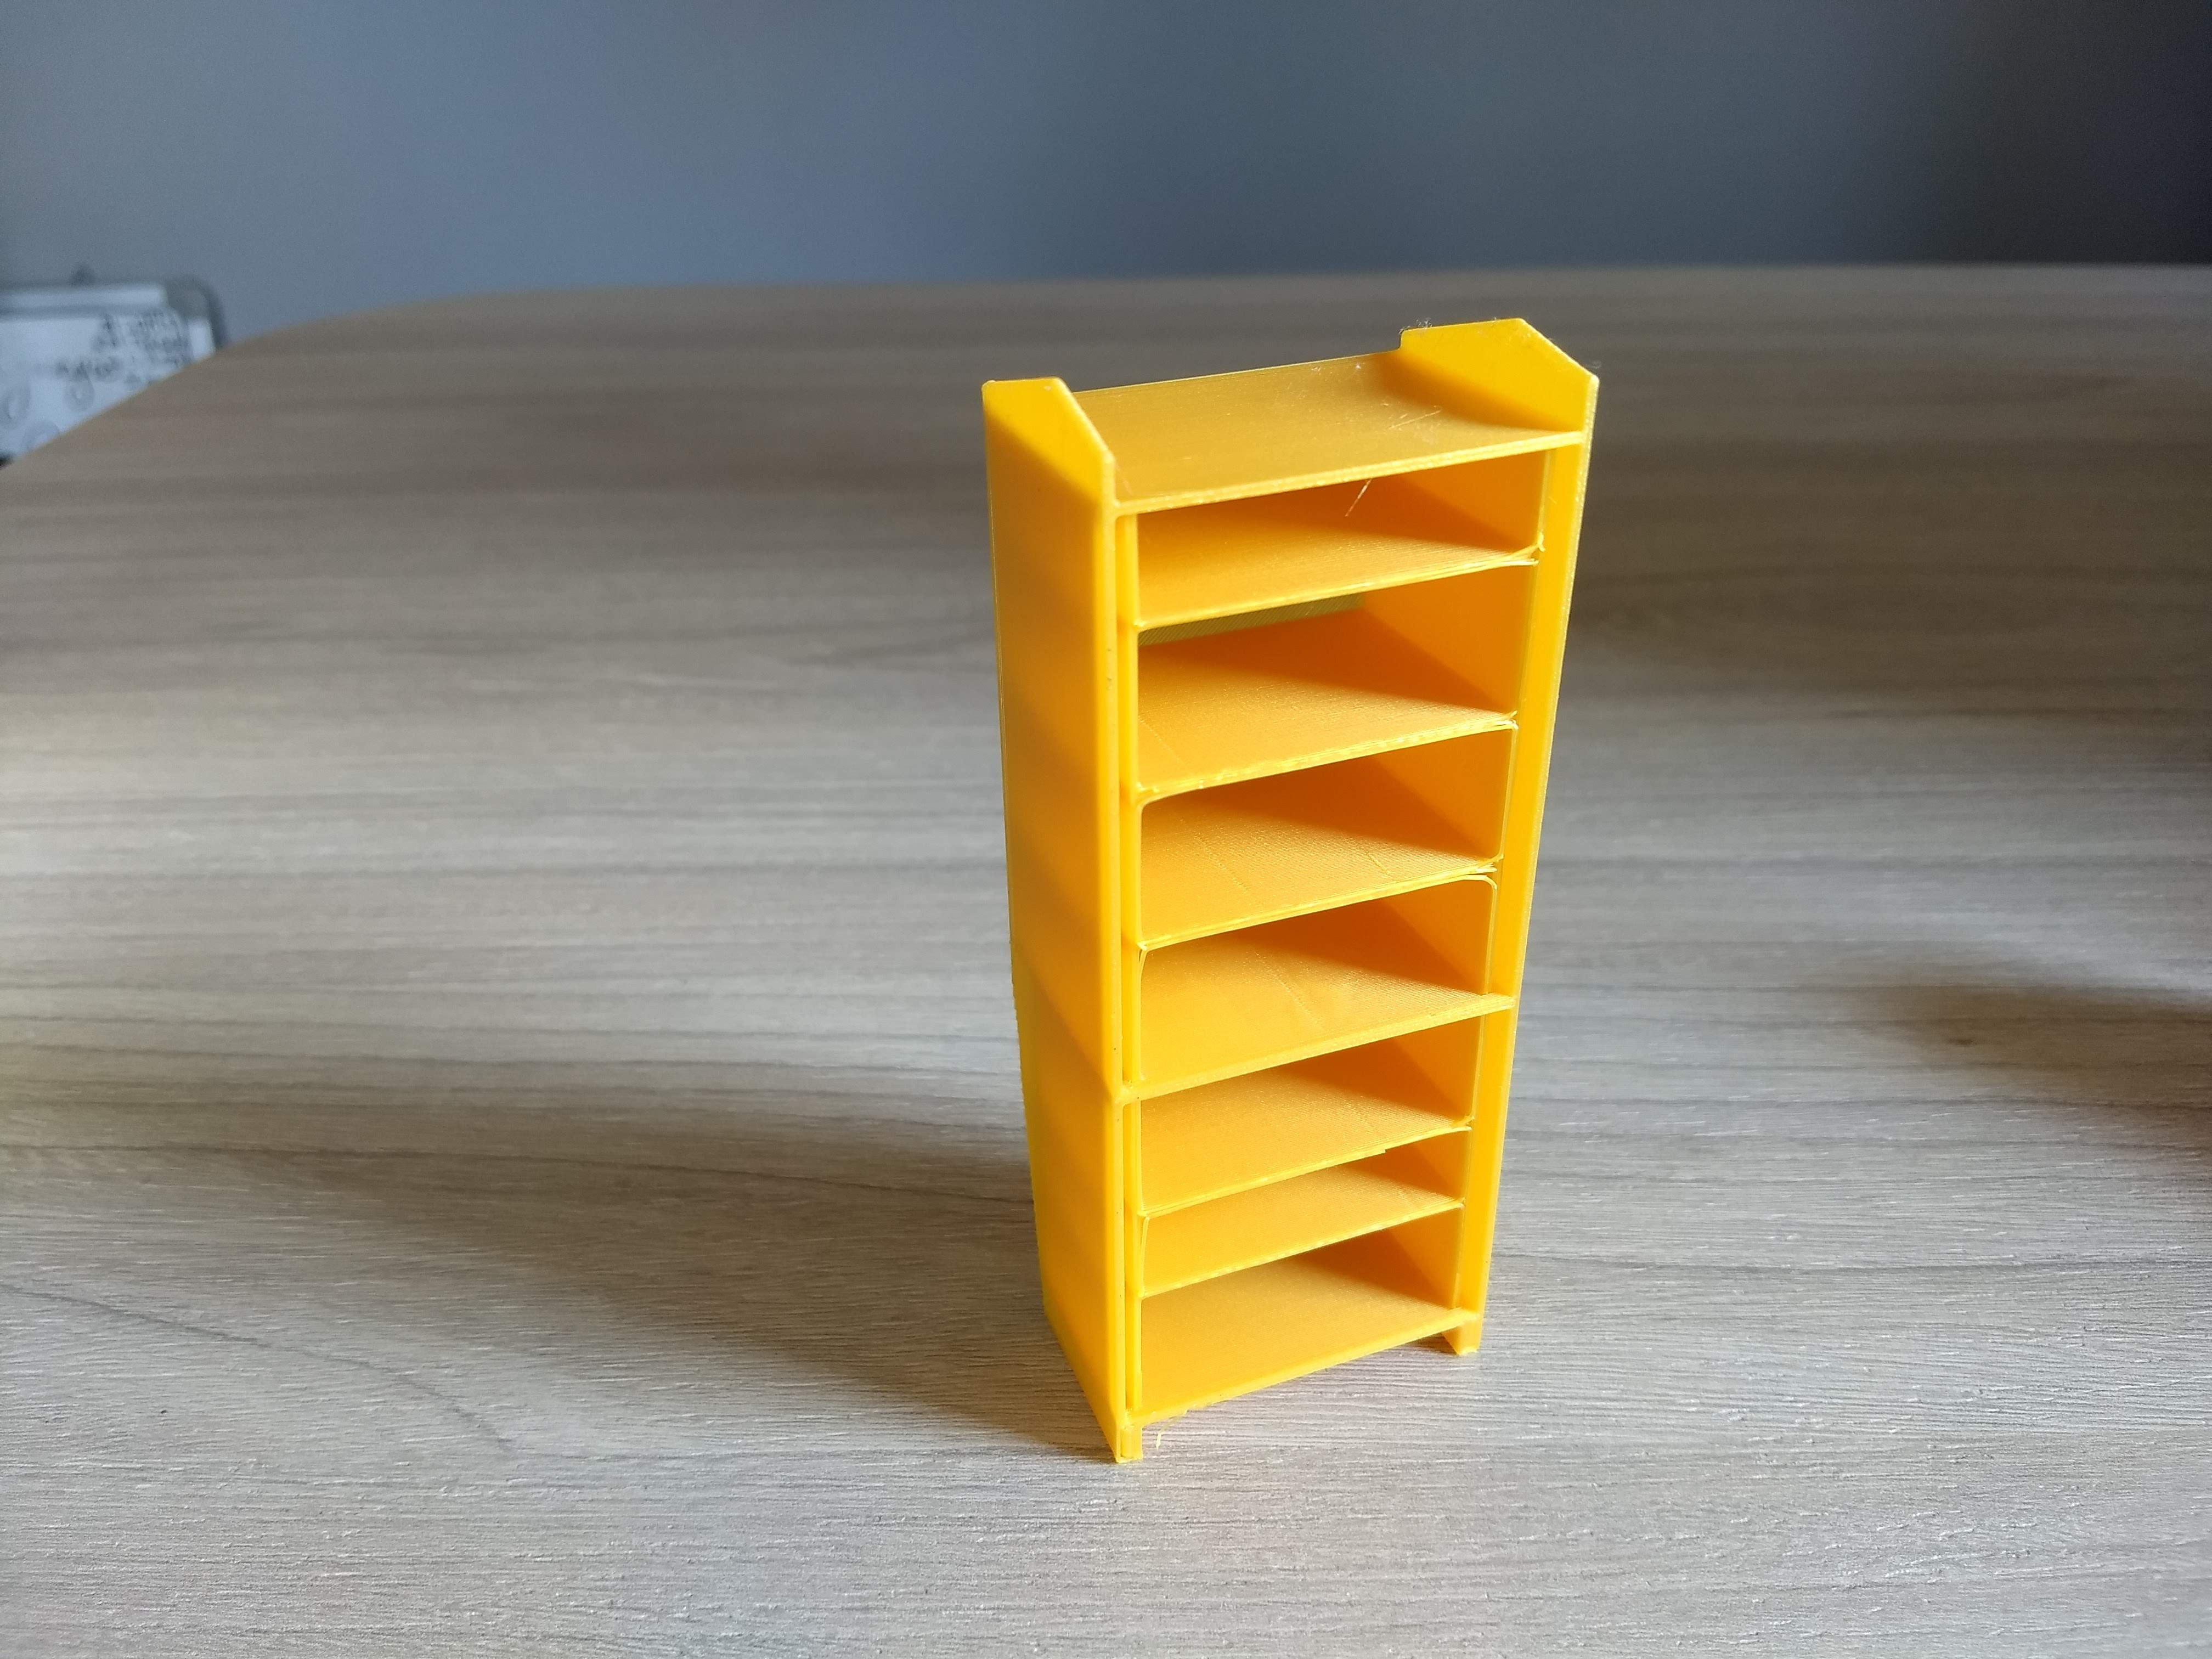
\includegraphics[width=1\linewidth]{43}
\end{figure}

